% Options for packages loaded elsewhere
\PassOptionsToPackage{unicode}{hyperref}
\PassOptionsToPackage{hyphens}{url}
\PassOptionsToPackage{dvipsnames,svgnames,x11names}{xcolor}
%
\documentclass[
  letterpaper,
  DIV=11,
  numbers=noendperiod]{scrreprt}

\usepackage{amsmath,amssymb}
\usepackage{iftex}
\ifPDFTeX
  \usepackage[T1]{fontenc}
  \usepackage[utf8]{inputenc}
  \usepackage{textcomp} % provide euro and other symbols
\else % if luatex or xetex
  \usepackage{unicode-math}
  \defaultfontfeatures{Scale=MatchLowercase}
  \defaultfontfeatures[\rmfamily]{Ligatures=TeX,Scale=1}
\fi
\usepackage{lmodern}
\ifPDFTeX\else  
    % xetex/luatex font selection
\fi
% Use upquote if available, for straight quotes in verbatim environments
\IfFileExists{upquote.sty}{\usepackage{upquote}}{}
\IfFileExists{microtype.sty}{% use microtype if available
  \usepackage[]{microtype}
  \UseMicrotypeSet[protrusion]{basicmath} % disable protrusion for tt fonts
}{}
\makeatletter
\@ifundefined{KOMAClassName}{% if non-KOMA class
  \IfFileExists{parskip.sty}{%
    \usepackage{parskip}
  }{% else
    \setlength{\parindent}{0pt}
    \setlength{\parskip}{6pt plus 2pt minus 1pt}}
}{% if KOMA class
  \KOMAoptions{parskip=half}}
\makeatother
\usepackage{xcolor}
\setlength{\emergencystretch}{3em} % prevent overfull lines
\setcounter{secnumdepth}{5}
% Make \paragraph and \subparagraph free-standing
\makeatletter
\ifx\paragraph\undefined\else
  \let\oldparagraph\paragraph
  \renewcommand{\paragraph}{
    \@ifstar
      \xxxParagraphStar
      \xxxParagraphNoStar
  }
  \newcommand{\xxxParagraphStar}[1]{\oldparagraph*{#1}\mbox{}}
  \newcommand{\xxxParagraphNoStar}[1]{\oldparagraph{#1}\mbox{}}
\fi
\ifx\subparagraph\undefined\else
  \let\oldsubparagraph\subparagraph
  \renewcommand{\subparagraph}{
    \@ifstar
      \xxxSubParagraphStar
      \xxxSubParagraphNoStar
  }
  \newcommand{\xxxSubParagraphStar}[1]{\oldsubparagraph*{#1}\mbox{}}
  \newcommand{\xxxSubParagraphNoStar}[1]{\oldsubparagraph{#1}\mbox{}}
\fi
\makeatother

\usepackage{color}
\usepackage{fancyvrb}
\newcommand{\VerbBar}{|}
\newcommand{\VERB}{\Verb[commandchars=\\\{\}]}
\DefineVerbatimEnvironment{Highlighting}{Verbatim}{commandchars=\\\{\}}
% Add ',fontsize=\small' for more characters per line
\usepackage{framed}
\definecolor{shadecolor}{RGB}{241,243,245}
\newenvironment{Shaded}{\begin{snugshade}}{\end{snugshade}}
\newcommand{\AlertTok}[1]{\textcolor[rgb]{0.68,0.00,0.00}{#1}}
\newcommand{\AnnotationTok}[1]{\textcolor[rgb]{0.37,0.37,0.37}{#1}}
\newcommand{\AttributeTok}[1]{\textcolor[rgb]{0.40,0.45,0.13}{#1}}
\newcommand{\BaseNTok}[1]{\textcolor[rgb]{0.68,0.00,0.00}{#1}}
\newcommand{\BuiltInTok}[1]{\textcolor[rgb]{0.00,0.23,0.31}{#1}}
\newcommand{\CharTok}[1]{\textcolor[rgb]{0.13,0.47,0.30}{#1}}
\newcommand{\CommentTok}[1]{\textcolor[rgb]{0.37,0.37,0.37}{#1}}
\newcommand{\CommentVarTok}[1]{\textcolor[rgb]{0.37,0.37,0.37}{\textit{#1}}}
\newcommand{\ConstantTok}[1]{\textcolor[rgb]{0.56,0.35,0.01}{#1}}
\newcommand{\ControlFlowTok}[1]{\textcolor[rgb]{0.00,0.23,0.31}{\textbf{#1}}}
\newcommand{\DataTypeTok}[1]{\textcolor[rgb]{0.68,0.00,0.00}{#1}}
\newcommand{\DecValTok}[1]{\textcolor[rgb]{0.68,0.00,0.00}{#1}}
\newcommand{\DocumentationTok}[1]{\textcolor[rgb]{0.37,0.37,0.37}{\textit{#1}}}
\newcommand{\ErrorTok}[1]{\textcolor[rgb]{0.68,0.00,0.00}{#1}}
\newcommand{\ExtensionTok}[1]{\textcolor[rgb]{0.00,0.23,0.31}{#1}}
\newcommand{\FloatTok}[1]{\textcolor[rgb]{0.68,0.00,0.00}{#1}}
\newcommand{\FunctionTok}[1]{\textcolor[rgb]{0.28,0.35,0.67}{#1}}
\newcommand{\ImportTok}[1]{\textcolor[rgb]{0.00,0.46,0.62}{#1}}
\newcommand{\InformationTok}[1]{\textcolor[rgb]{0.37,0.37,0.37}{#1}}
\newcommand{\KeywordTok}[1]{\textcolor[rgb]{0.00,0.23,0.31}{\textbf{#1}}}
\newcommand{\NormalTok}[1]{\textcolor[rgb]{0.00,0.23,0.31}{#1}}
\newcommand{\OperatorTok}[1]{\textcolor[rgb]{0.37,0.37,0.37}{#1}}
\newcommand{\OtherTok}[1]{\textcolor[rgb]{0.00,0.23,0.31}{#1}}
\newcommand{\PreprocessorTok}[1]{\textcolor[rgb]{0.68,0.00,0.00}{#1}}
\newcommand{\RegionMarkerTok}[1]{\textcolor[rgb]{0.00,0.23,0.31}{#1}}
\newcommand{\SpecialCharTok}[1]{\textcolor[rgb]{0.37,0.37,0.37}{#1}}
\newcommand{\SpecialStringTok}[1]{\textcolor[rgb]{0.13,0.47,0.30}{#1}}
\newcommand{\StringTok}[1]{\textcolor[rgb]{0.13,0.47,0.30}{#1}}
\newcommand{\VariableTok}[1]{\textcolor[rgb]{0.07,0.07,0.07}{#1}}
\newcommand{\VerbatimStringTok}[1]{\textcolor[rgb]{0.13,0.47,0.30}{#1}}
\newcommand{\WarningTok}[1]{\textcolor[rgb]{0.37,0.37,0.37}{\textit{#1}}}

\providecommand{\tightlist}{%
  \setlength{\itemsep}{0pt}\setlength{\parskip}{0pt}}\usepackage{longtable,booktabs,array}
\usepackage{calc} % for calculating minipage widths
% Correct order of tables after \paragraph or \subparagraph
\usepackage{etoolbox}
\makeatletter
\patchcmd\longtable{\par}{\if@noskipsec\mbox{}\fi\par}{}{}
\makeatother
% Allow footnotes in longtable head/foot
\IfFileExists{footnotehyper.sty}{\usepackage{footnotehyper}}{\usepackage{footnote}}
\makesavenoteenv{longtable}
\usepackage{graphicx}
\makeatletter
\def\maxwidth{\ifdim\Gin@nat@width>\linewidth\linewidth\else\Gin@nat@width\fi}
\def\maxheight{\ifdim\Gin@nat@height>\textheight\textheight\else\Gin@nat@height\fi}
\makeatother
% Scale images if necessary, so that they will not overflow the page
% margins by default, and it is still possible to overwrite the defaults
% using explicit options in \includegraphics[width, height, ...]{}
\setkeys{Gin}{width=\maxwidth,height=\maxheight,keepaspectratio}
% Set default figure placement to htbp
\makeatletter
\def\fps@figure{htbp}
\makeatother
% definitions for citeproc citations
\NewDocumentCommand\citeproctext{}{}
\NewDocumentCommand\citeproc{mm}{%
  \begingroup\def\citeproctext{#2}\cite{#1}\endgroup}
\makeatletter
 % allow citations to break across lines
 \let\@cite@ofmt\@firstofone
 % avoid brackets around text for \cite:
 \def\@biblabel#1{}
 \def\@cite#1#2{{#1\if@tempswa , #2\fi}}
\makeatother
\newlength{\cslhangindent}
\setlength{\cslhangindent}{1.5em}
\newlength{\csllabelwidth}
\setlength{\csllabelwidth}{3em}
\newenvironment{CSLReferences}[2] % #1 hanging-indent, #2 entry-spacing
 {\begin{list}{}{%
  \setlength{\itemindent}{0pt}
  \setlength{\leftmargin}{0pt}
  \setlength{\parsep}{0pt}
  % turn on hanging indent if param 1 is 1
  \ifodd #1
   \setlength{\leftmargin}{\cslhangindent}
   \setlength{\itemindent}{-1\cslhangindent}
  \fi
  % set entry spacing
  \setlength{\itemsep}{#2\baselineskip}}}
 {\end{list}}
\usepackage{calc}
\newcommand{\CSLBlock}[1]{\hfill\break\parbox[t]{\linewidth}{\strut\ignorespaces#1\strut}}
\newcommand{\CSLLeftMargin}[1]{\parbox[t]{\csllabelwidth}{\strut#1\strut}}
\newcommand{\CSLRightInline}[1]{\parbox[t]{\linewidth - \csllabelwidth}{\strut#1\strut}}
\newcommand{\CSLIndent}[1]{\hspace{\cslhangindent}#1}

\KOMAoption{captions}{tableheading}
\makeatletter
\@ifpackageloaded{tcolorbox}{}{\usepackage[skins,breakable]{tcolorbox}}
\@ifpackageloaded{fontawesome5}{}{\usepackage{fontawesome5}}
\definecolor{quarto-callout-color}{HTML}{909090}
\definecolor{quarto-callout-note-color}{HTML}{0758E5}
\definecolor{quarto-callout-important-color}{HTML}{CC1914}
\definecolor{quarto-callout-warning-color}{HTML}{EB9113}
\definecolor{quarto-callout-tip-color}{HTML}{00A047}
\definecolor{quarto-callout-caution-color}{HTML}{FC5300}
\definecolor{quarto-callout-color-frame}{HTML}{acacac}
\definecolor{quarto-callout-note-color-frame}{HTML}{4582ec}
\definecolor{quarto-callout-important-color-frame}{HTML}{d9534f}
\definecolor{quarto-callout-warning-color-frame}{HTML}{f0ad4e}
\definecolor{quarto-callout-tip-color-frame}{HTML}{02b875}
\definecolor{quarto-callout-caution-color-frame}{HTML}{fd7e14}
\makeatother
\makeatletter
\@ifpackageloaded{bookmark}{}{\usepackage{bookmark}}
\makeatother
\makeatletter
\@ifpackageloaded{caption}{}{\usepackage{caption}}
\AtBeginDocument{%
\ifdefined\contentsname
  \renewcommand*\contentsname{Table of contents}
\else
  \newcommand\contentsname{Table of contents}
\fi
\ifdefined\listfigurename
  \renewcommand*\listfigurename{List of Figures}
\else
  \newcommand\listfigurename{List of Figures}
\fi
\ifdefined\listtablename
  \renewcommand*\listtablename{List of Tables}
\else
  \newcommand\listtablename{List of Tables}
\fi
\ifdefined\figurename
  \renewcommand*\figurename{Figure}
\else
  \newcommand\figurename{Figure}
\fi
\ifdefined\tablename
  \renewcommand*\tablename{Table}
\else
  \newcommand\tablename{Table}
\fi
}
\@ifpackageloaded{float}{}{\usepackage{float}}
\floatstyle{ruled}
\@ifundefined{c@chapter}{\newfloat{codelisting}{h}{lop}}{\newfloat{codelisting}{h}{lop}[chapter]}
\floatname{codelisting}{Listing}
\newcommand*\listoflistings{\listof{codelisting}{List of Listings}}
\usepackage{amsthm}
\theoremstyle{definition}
\newtheorem{exercise}{Exercise}[chapter]
\theoremstyle{remark}
\AtBeginDocument{\renewcommand*{\proofname}{Proof}}
\newtheorem*{remark}{Remark}
\newtheorem*{solution}{Solution}
\newtheorem{refremark}{Remark}[chapter]
\newtheorem{refsolution}{Solution}[chapter]
\makeatother
\makeatletter
\makeatother
\makeatletter
\@ifpackageloaded{caption}{}{\usepackage{caption}}
\@ifpackageloaded{subcaption}{}{\usepackage{subcaption}}
\makeatother
\newcounter{quartocallouttipno}
\newcommand{\quartocallouttip}[1]{\refstepcounter{quartocallouttipno}\label{#1}}

\ifLuaTeX
  \usepackage{selnolig}  % disable illegal ligatures
\fi
\usepackage{bookmark}

\IfFileExists{xurl.sty}{\usepackage{xurl}}{} % add URL line breaks if available
\urlstyle{same} % disable monospaced font for URLs
\hypersetup{
  pdftitle={Modeling Life},
  pdfauthor={Theoretical Biology Group, Utrecht University},
  colorlinks=true,
  linkcolor={blue},
  filecolor={Maroon},
  citecolor={Blue},
  urlcolor={Blue},
  pdfcreator={LaTeX via pandoc}}


\title{Modeling Life}
\author{Theoretical Biology Group, Utrecht University}
\date{2025-04-24}

\begin{document}
\maketitle

\renewcommand*\contentsname{Table of contents}
{
\hypersetup{linkcolor=}
\setcounter{tocdepth}{2}
\tableofcontents
}

\chapter*{Modeling life}\label{modeling}
\addcontentsline{toc}{chapter}{Modeling life}

\markboth{Modeling life}{Modeling life}

Welcome to the course Modeling Life.

\part{Course information}

\chapter{Quarto examples}\label{quarto-examples}

\section{Equations}\label{equations}

Here's an equation:

\begin{equation}\phantomsection\label{eq-log}{ 
\frac{\mathrm{d}N}{\mathrm{d}t} = rN(1 - \frac{N}{K}) 
}\end{equation}

And Equation~\ref{eq-log} is a reference to the equation above.

\section{References}\label{references}

See Knuth (1984) for additional discussion of literate programming.

\section{Syntax highlighting}\label{syntax-highlighting}

Here's some python code:

\begin{Shaded}
\begin{Highlighting}[]
\ImportTok{import}\NormalTok{ numpy }\ImportTok{as}\NormalTok{ np}
\NormalTok{np.random.seed(}\DecValTok{42}\NormalTok{)}
\NormalTok{a }\OperatorTok{=} \DecValTok{1} \OperatorTok{+} \DecValTok{2}
\NormalTok{b }\OperatorTok{=}\NormalTok{ a }\OperatorTok{+} \DecValTok{3}
\BuiltInTok{print}\NormalTok{(}\StringTok{"Hello"}\NormalTok{)}
\end{Highlighting}
\end{Shaded}

\section{Visualising data (R)}\label{visualising-data-r}

Here's an interactive plot generated with R:

\includegraphics{intro_files/figure-pdf/unnamed-chunk-1-1.pdf}

\section{A youtube clip:}\label{a-youtube-clip}

\url{https://www.youtube.com/embed/wo9vZccmqwc}

\section{An `iframe' to a different page (e.g.~my
simulations)}\label{an-iframe-to-a-different-page-e.g.-my-simulations}

\subsection{Mermaid}\label{mermaid}

Diagrams (Mermaid syntax):

\begin{figure}

\centering{

\includegraphics[width=7.47in,height=2.27in]{intro_files/figure-latex/mermaid-figure-1.png}

}

\caption{\label{fig-variables}Types of models}

\end{figure}%

Which can be referred to Figure~\ref{fig-variables}.

\subsection{Callouts}\label{callouts}

Call-outs can organise information and highlight important points.

\begin{tcolorbox}[enhanced jigsaw, leftrule=.75mm, colbacktitle=quarto-callout-note-color!10!white, coltitle=black, colback=white, left=2mm, bottomtitle=1mm, arc=.35mm, titlerule=0mm, breakable, bottomrule=.15mm, opacitybacktitle=0.6, colframe=quarto-callout-note-color-frame, title=\textcolor{quarto-callout-note-color}{\faInfo}\hspace{0.5em}{Note}, opacityback=0, toprule=.15mm, toptitle=1mm, rightrule=.15mm]

Note that there are five types of callouts, including: \texttt{note},
\texttt{warning}, \texttt{important}, \texttt{tip}, and
\texttt{caution}.

\end{tcolorbox}

\begin{tcolorbox}[enhanced jigsaw, leftrule=.75mm, colbacktitle=quarto-callout-tip-color!10!white, coltitle=black, colback=white, left=2mm, bottomtitle=1mm, arc=.35mm, titlerule=0mm, breakable, bottomrule=.15mm, opacitybacktitle=0.6, colframe=quarto-callout-tip-color-frame, title=\textcolor{quarto-callout-tip-color}{\faLightbulb}\hspace{0.5em}{Tip with Title}, opacityback=0, toprule=.15mm, toptitle=1mm, rightrule=.15mm]

This is an example of a callout with a title.

\end{tcolorbox}

\begin{tcolorbox}[enhanced jigsaw, leftrule=.75mm, colbacktitle=quarto-callout-caution-color!10!white, coltitle=black, colback=white, left=2mm, bottomtitle=1mm, arc=.35mm, titlerule=0mm, breakable, bottomrule=.15mm, opacitybacktitle=0.6, colframe=quarto-callout-caution-color-frame, title=\textcolor{quarto-callout-caution-color}{\faFire}\hspace{0.5em}{Expand To Learn About Collapse}, opacityback=0, toprule=.15mm, toptitle=1mm, rightrule=.15mm]

This is an example of a `folded' caution callout that can be expanded by
the user. You can use \texttt{collapse="true"} to collapse it by default
or \texttt{collapse="false"} to make a collapsible callout that is
expanded by default.

\end{tcolorbox}

\begin{tcolorbox}[enhanced jigsaw, leftrule=.75mm, colbacktitle=quarto-callout-tip-color!10!white, coltitle=black, colback=white, left=2mm, bottomtitle=1mm, arc=.35mm, titlerule=0mm, breakable, bottomrule=.15mm, opacitybacktitle=0.6, colframe=quarto-callout-tip-color-frame, title=\textcolor{quarto-callout-tip-color}{\faLightbulb}\hspace{0.5em}{Tip \ref*{tip-example}: Cross-Referencing a Tip}, opacityback=0, toprule=.15mm, toptitle=1mm, rightrule=.15mm]

\quartocallouttip{tip-example} 

Add an ID starting with \texttt{\#tip-} to reference a tip.

\end{tcolorbox}

See Tip~\ref{tip-example}\ldots{}

\subsection{How to format questions/problem
sets}\label{how-to-format-questionsproblem-sets}

\begin{exercise}[Test
1]\protect\hypertarget{exr-test1}{}\label{exr-test1}

The equation of any straight line, called a linear equation, can be
written as:

\begin{equation}\phantomsection\label{eq-line}{ 
y = mx + b
}\end{equation}

Refer to the equation like this Equation~\ref{eq-line} or like
Customlabel~\ref{eq-line}.

\textbf{a.} Blabla?

\textbf{b.} Of blablabla?

\end{exercise}

\subsection{Sharing data tables:}\label{sharing-data-tables}

\includegraphics{intro_files/figure-pdf/tab-anscombe-1.pdf}

\chapter{General course info}\label{general}

Our names, email addresses, an overview of the course content, learning
goals, tips, grading, group formation, usage of Brightspace, materials
they need, required attendencee, and feedback is welcome blabla.

\chapter{Schedule}\label{modelling}

The schedule of the course and important deadlines are outlined below.
The course is divided into blabla modules, each with its own set of
topics and blabla. The schedule is subject to change, and any updates
will be communicated in advance. Blabla.

(paste below is the schedule of Kwanti/BioMS as an example)

\begin{verbatim}
file:////private/var/folders/22/dvqytf_15mqgwc9rn9l42y5w0000gn/T/RtmpyTgHQy/file7b6f4bc0af09/widget7b6f57239eb9.html screenshot completed
\end{verbatim}

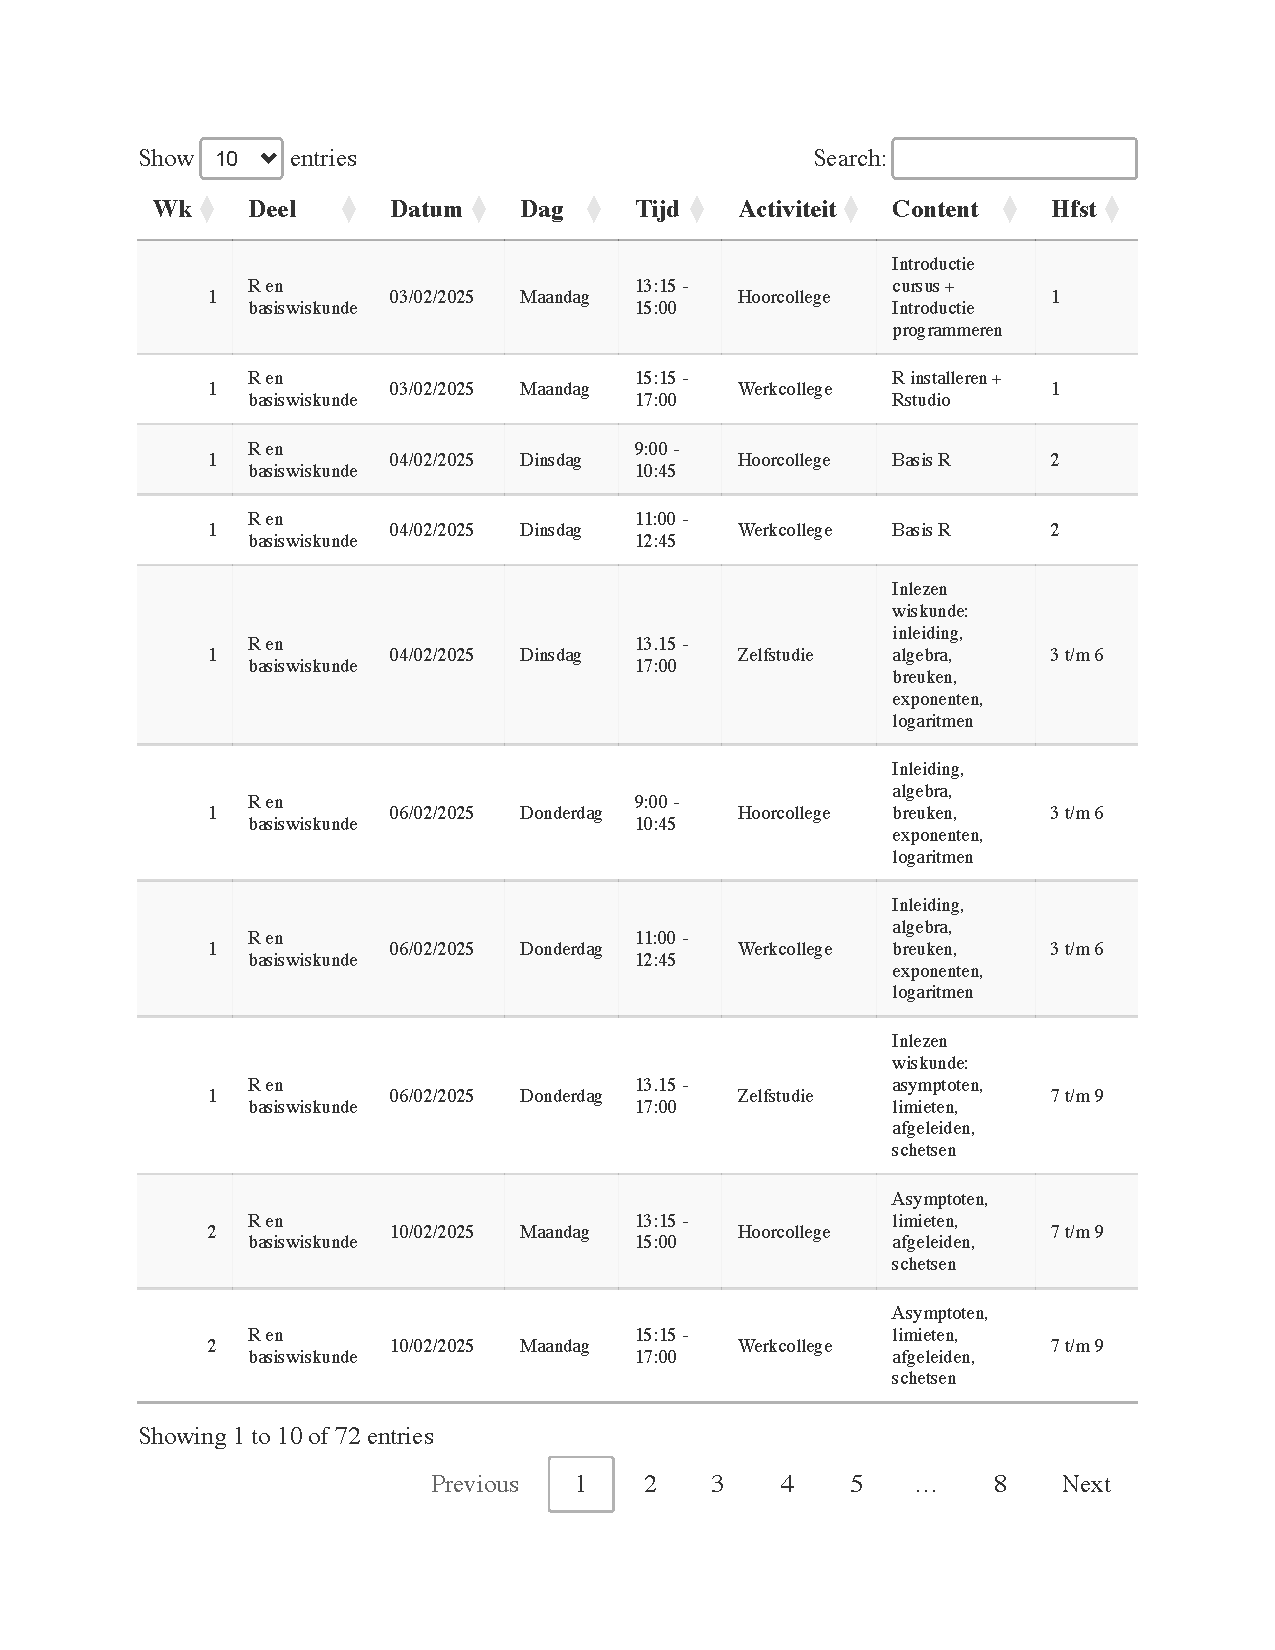
\includegraphics{schedule_files/figure-pdf/unnamed-chunk-1-1.pdf}

\part{I) Pattern formation}

\chapter{Pattern formation}\label{pattern-formation}

\section{Equations}\label{equations-1}

Here's an equation:

\begin{equation}\phantomsection\label{eq-log}{ 
\frac{\mathrm{d}N}{\mathrm{d}t} = rN(1 - \frac{N}{K}) 
}\end{equation}

And Equation~\ref{eq-log} is a reference to the equation above.

\section{References}\label{references-1}

See Knuth (1984) for additional discussion of literate programming.

\section{Syntax highlighting}\label{syntax-highlighting-1}

Here's some python code:

\begin{Shaded}
\begin{Highlighting}[]
\ImportTok{import}\NormalTok{ numpy }\ImportTok{as}\NormalTok{ np}
\NormalTok{np.random.seed(}\DecValTok{42}\NormalTok{)}
\NormalTok{a }\OperatorTok{=} \DecValTok{1} \OperatorTok{+} \DecValTok{2}
\NormalTok{b }\OperatorTok{=}\NormalTok{ a }\OperatorTok{+} \DecValTok{3}
\BuiltInTok{print}\NormalTok{(}\StringTok{"Hello"}\NormalTok{)}
\end{Highlighting}
\end{Shaded}

\section{Visualising data (R)}\label{visualising-data-r-1}

Here's an interactive plot generated with R:

\includegraphics{pattern_intro_text_files/figure-pdf/unnamed-chunk-1-1.pdf}

\section{A youtube clip:}\label{a-youtube-clip-1}

\url{https://www.youtube.com/embed/wo9vZccmqwc}

\section{An `iframe' to a different page (e.g.~my
simulations)}\label{an-iframe-to-a-different-page-e.g.-my-simulations-1}

\subsection{Mermaid}\label{mermaid-1}

Diagrams (Mermaid syntax):

\begin{figure}

\centering{

\includegraphics[width=7.47in,height=2.27in]{pattern_intro_text_files/figure-latex/mermaid-figure-1.png}

}

\caption{\label{fig-variables}Types of models}

\end{figure}%

Which can be referred to Figure~\ref{fig-variables}.

\subsection{Callouts}\label{callouts-1}

Call-outs can organise information and highlight important points.

\begin{tcolorbox}[enhanced jigsaw, leftrule=.75mm, colbacktitle=quarto-callout-note-color!10!white, coltitle=black, colback=white, left=2mm, bottomtitle=1mm, arc=.35mm, titlerule=0mm, breakable, bottomrule=.15mm, opacitybacktitle=0.6, colframe=quarto-callout-note-color-frame, title=\textcolor{quarto-callout-note-color}{\faInfo}\hspace{0.5em}{Note}, opacityback=0, toprule=.15mm, toptitle=1mm, rightrule=.15mm]

Note that there are five types of callouts, including: \texttt{note},
\texttt{warning}, \texttt{important}, \texttt{tip}, and
\texttt{caution}.

\end{tcolorbox}

\begin{tcolorbox}[enhanced jigsaw, leftrule=.75mm, colbacktitle=quarto-callout-tip-color!10!white, coltitle=black, colback=white, left=2mm, bottomtitle=1mm, arc=.35mm, titlerule=0mm, breakable, bottomrule=.15mm, opacitybacktitle=0.6, colframe=quarto-callout-tip-color-frame, title=\textcolor{quarto-callout-tip-color}{\faLightbulb}\hspace{0.5em}{Tip with Title}, opacityback=0, toprule=.15mm, toptitle=1mm, rightrule=.15mm]

This is an example of a callout with a title.

\end{tcolorbox}

\begin{tcolorbox}[enhanced jigsaw, leftrule=.75mm, colbacktitle=quarto-callout-caution-color!10!white, coltitle=black, colback=white, left=2mm, bottomtitle=1mm, arc=.35mm, titlerule=0mm, breakable, bottomrule=.15mm, opacitybacktitle=0.6, colframe=quarto-callout-caution-color-frame, title=\textcolor{quarto-callout-caution-color}{\faFire}\hspace{0.5em}{Expand To Learn About Collapse}, opacityback=0, toprule=.15mm, toptitle=1mm, rightrule=.15mm]

This is an example of a `folded' caution callout that can be expanded by
the user. You can use \texttt{collapse="true"} to collapse it by default
or \texttt{collapse="false"} to make a collapsible callout that is
expanded by default.

\end{tcolorbox}

\begin{tcolorbox}[enhanced jigsaw, leftrule=.75mm, colbacktitle=quarto-callout-tip-color!10!white, coltitle=black, colback=white, left=2mm, bottomtitle=1mm, arc=.35mm, titlerule=0mm, breakable, bottomrule=.15mm, opacitybacktitle=0.6, colframe=quarto-callout-tip-color-frame, title=\textcolor{quarto-callout-tip-color}{\faLightbulb}\hspace{0.5em}{Tip \ref*{tip-example}: Cross-Referencing a Tip}, opacityback=0, toprule=.15mm, toptitle=1mm, rightrule=.15mm]

\quartocallouttip{tip-example} 

Add an ID starting with \texttt{\#tip-} to reference a tip.

\end{tcolorbox}

See Tip~\ref{tip-example}\ldots{}

\subsection{How to format questions/problem
sets}\label{how-to-format-questionsproblem-sets-1}

\begin{exercise}[Test
1]\protect\hypertarget{exr-test1}{}\label{exr-test1}

The equation of any straight line, called a linear equation, can be
written as:

\begin{equation}\phantomsection\label{eq-line}{ 
y = mx + b
}\end{equation}

Refer to the equation like this Equation~\ref{eq-line} or like
Customlabel~\ref{eq-line}.

\textbf{a.} Blabla?

\textbf{b.} Of blablabla?

\end{exercise}

\subsection{Sharing data tables:}\label{sharing-data-tables-1}

\includegraphics{pattern_intro_text_files/figure-pdf/tab-anscombe-1.pdf}

\chapter{Practical 1}\label{practical-1}

\section{Equations}\label{equations-2}

Here's an equation:

\begin{equation}\phantomsection\label{eq-log}{ 
\frac{\mathrm{d}N}{\mathrm{d}t} = rN(1 - \frac{N}{K}) 
}\end{equation}

And Equation~\ref{eq-log} is a reference to the equation above.

\section{References}\label{references-2}

See Knuth (1984) for additional discussion of literate programming.

\section{Syntax highlighting}\label{syntax-highlighting-2}

Here's some python code:

\begin{Shaded}
\begin{Highlighting}[]
\ImportTok{import}\NormalTok{ numpy }\ImportTok{as}\NormalTok{ np}
\NormalTok{np.random.seed(}\DecValTok{42}\NormalTok{)}
\NormalTok{a }\OperatorTok{=} \DecValTok{1} \OperatorTok{+} \DecValTok{2}
\NormalTok{b }\OperatorTok{=}\NormalTok{ a }\OperatorTok{+} \DecValTok{3}
\BuiltInTok{print}\NormalTok{(}\StringTok{"Hello"}\NormalTok{)}
\end{Highlighting}
\end{Shaded}

\section{Visualising data (R)}\label{visualising-data-r-2}

Here's an interactive plot generated with R:

\includegraphics{pattern_practical_1_files/figure-pdf/unnamed-chunk-1-1.pdf}

\section{A youtube clip:}\label{a-youtube-clip-2}

\url{https://www.youtube.com/embed/wo9vZccmqwc}

\section{An `iframe' to a different page (e.g.~my
simulations)}\label{an-iframe-to-a-different-page-e.g.-my-simulations-2}

\subsection{Mermaid}\label{mermaid-2}

Diagrams (Mermaid syntax):

\begin{figure}

\centering{

\includegraphics[width=7.47in,height=2.27in]{pattern_practical_1_files/figure-latex/mermaid-figure-1.png}

}

\caption{\label{fig-variables}Types of models}

\end{figure}%

Which can be referred to Figure~\ref{fig-variables}.

\subsection{Callouts}\label{callouts-2}

Call-outs can organise information and highlight important points.

\begin{tcolorbox}[enhanced jigsaw, leftrule=.75mm, colbacktitle=quarto-callout-note-color!10!white, coltitle=black, colback=white, left=2mm, bottomtitle=1mm, arc=.35mm, titlerule=0mm, breakable, bottomrule=.15mm, opacitybacktitle=0.6, colframe=quarto-callout-note-color-frame, title=\textcolor{quarto-callout-note-color}{\faInfo}\hspace{0.5em}{Note}, opacityback=0, toprule=.15mm, toptitle=1mm, rightrule=.15mm]

Note that there are five types of callouts, including: \texttt{note},
\texttt{warning}, \texttt{important}, \texttt{tip}, and
\texttt{caution}.

\end{tcolorbox}

\begin{tcolorbox}[enhanced jigsaw, leftrule=.75mm, colbacktitle=quarto-callout-tip-color!10!white, coltitle=black, colback=white, left=2mm, bottomtitle=1mm, arc=.35mm, titlerule=0mm, breakable, bottomrule=.15mm, opacitybacktitle=0.6, colframe=quarto-callout-tip-color-frame, title=\textcolor{quarto-callout-tip-color}{\faLightbulb}\hspace{0.5em}{Tip with Title}, opacityback=0, toprule=.15mm, toptitle=1mm, rightrule=.15mm]

This is an example of a callout with a title.

\end{tcolorbox}

\begin{tcolorbox}[enhanced jigsaw, leftrule=.75mm, colbacktitle=quarto-callout-caution-color!10!white, coltitle=black, colback=white, left=2mm, bottomtitle=1mm, arc=.35mm, titlerule=0mm, breakable, bottomrule=.15mm, opacitybacktitle=0.6, colframe=quarto-callout-caution-color-frame, title=\textcolor{quarto-callout-caution-color}{\faFire}\hspace{0.5em}{Expand To Learn About Collapse}, opacityback=0, toprule=.15mm, toptitle=1mm, rightrule=.15mm]

This is an example of a `folded' caution callout that can be expanded by
the user. You can use \texttt{collapse="true"} to collapse it by default
or \texttt{collapse="false"} to make a collapsible callout that is
expanded by default.

\end{tcolorbox}

\begin{tcolorbox}[enhanced jigsaw, leftrule=.75mm, colbacktitle=quarto-callout-tip-color!10!white, coltitle=black, colback=white, left=2mm, bottomtitle=1mm, arc=.35mm, titlerule=0mm, breakable, bottomrule=.15mm, opacitybacktitle=0.6, colframe=quarto-callout-tip-color-frame, title=\textcolor{quarto-callout-tip-color}{\faLightbulb}\hspace{0.5em}{Tip \ref*{tip-example}: Cross-Referencing a Tip}, opacityback=0, toprule=.15mm, toptitle=1mm, rightrule=.15mm]

\quartocallouttip{tip-example} 

Add an ID starting with \texttt{\#tip-} to reference a tip.

\end{tcolorbox}

See Tip~\ref{tip-example}\ldots{}

\subsection{How to format questions/problem
sets}\label{how-to-format-questionsproblem-sets-2}

\begin{exercise}[Test
1]\protect\hypertarget{exr-test1}{}\label{exr-test1}

The equation of any straight line, called a linear equation, can be
written as:

\begin{equation}\phantomsection\label{eq-line}{ 
y = mx + b
}\end{equation}

Refer to the equation like this Equation~\ref{eq-line} or like
Customlabel~\ref{eq-line}.

\textbf{a.} Blabla?

\textbf{b.} Of blablabla?

\end{exercise}

\subsection{Sharing data tables:}\label{sharing-data-tables-2}

\includegraphics{pattern_practical_1_files/figure-pdf/tab-anscombe-1.pdf}

\chapter{Practical 2}\label{practical-2}

\section{Equations}\label{equations-3}

Here's an equation:

\begin{equation}\phantomsection\label{eq-log}{ 
\frac{\mathrm{d}N}{\mathrm{d}t} = rN(1 - \frac{N}{K}) 
}\end{equation}

And Equation~\ref{eq-log} is a reference to the equation above.

\section{References}\label{references-3}

See Knuth (1984) for additional discussion of literate programming.

\section{Syntax highlighting}\label{syntax-highlighting-3}

Here's some python code:

\begin{Shaded}
\begin{Highlighting}[]
\ImportTok{import}\NormalTok{ numpy }\ImportTok{as}\NormalTok{ np}
\NormalTok{np.random.seed(}\DecValTok{42}\NormalTok{)}
\NormalTok{a }\OperatorTok{=} \DecValTok{1} \OperatorTok{+} \DecValTok{2}
\NormalTok{b }\OperatorTok{=}\NormalTok{ a }\OperatorTok{+} \DecValTok{3}
\BuiltInTok{print}\NormalTok{(}\StringTok{"Hello"}\NormalTok{)}
\end{Highlighting}
\end{Shaded}

\section{Visualising data (R)}\label{visualising-data-r-3}

Here's an interactive plot generated with R:

\includegraphics{pattern_practical_2_files/figure-pdf/unnamed-chunk-1-1.pdf}

\section{A youtube clip:}\label{a-youtube-clip-3}

\url{https://www.youtube.com/embed/wo9vZccmqwc}

\section{An `iframe' to a different page (e.g.~my
simulations)}\label{an-iframe-to-a-different-page-e.g.-my-simulations-3}

\subsection{Mermaid}\label{mermaid-3}

Diagrams (Mermaid syntax):

\begin{figure}

\centering{

\includegraphics[width=7.47in,height=2.27in]{pattern_practical_2_files/figure-latex/mermaid-figure-1.png}

}

\caption{\label{fig-variables}Types of models}

\end{figure}%

Which can be referred to Figure~\ref{fig-variables}.

\subsection{Callouts}\label{callouts-3}

Call-outs can organise information and highlight important points.

\begin{tcolorbox}[enhanced jigsaw, leftrule=.75mm, colbacktitle=quarto-callout-note-color!10!white, coltitle=black, colback=white, left=2mm, bottomtitle=1mm, arc=.35mm, titlerule=0mm, breakable, bottomrule=.15mm, opacitybacktitle=0.6, colframe=quarto-callout-note-color-frame, title=\textcolor{quarto-callout-note-color}{\faInfo}\hspace{0.5em}{Note}, opacityback=0, toprule=.15mm, toptitle=1mm, rightrule=.15mm]

Note that there are five types of callouts, including: \texttt{note},
\texttt{warning}, \texttt{important}, \texttt{tip}, and
\texttt{caution}.

\end{tcolorbox}

\begin{tcolorbox}[enhanced jigsaw, leftrule=.75mm, colbacktitle=quarto-callout-tip-color!10!white, coltitle=black, colback=white, left=2mm, bottomtitle=1mm, arc=.35mm, titlerule=0mm, breakable, bottomrule=.15mm, opacitybacktitle=0.6, colframe=quarto-callout-tip-color-frame, title=\textcolor{quarto-callout-tip-color}{\faLightbulb}\hspace{0.5em}{Tip with Title}, opacityback=0, toprule=.15mm, toptitle=1mm, rightrule=.15mm]

This is an example of a callout with a title.

\end{tcolorbox}

\begin{tcolorbox}[enhanced jigsaw, leftrule=.75mm, colbacktitle=quarto-callout-caution-color!10!white, coltitle=black, colback=white, left=2mm, bottomtitle=1mm, arc=.35mm, titlerule=0mm, breakable, bottomrule=.15mm, opacitybacktitle=0.6, colframe=quarto-callout-caution-color-frame, title=\textcolor{quarto-callout-caution-color}{\faFire}\hspace{0.5em}{Expand To Learn About Collapse}, opacityback=0, toprule=.15mm, toptitle=1mm, rightrule=.15mm]

This is an example of a `folded' caution callout that can be expanded by
the user. You can use \texttt{collapse="true"} to collapse it by default
or \texttt{collapse="false"} to make a collapsible callout that is
expanded by default.

\end{tcolorbox}

\begin{tcolorbox}[enhanced jigsaw, leftrule=.75mm, colbacktitle=quarto-callout-tip-color!10!white, coltitle=black, colback=white, left=2mm, bottomtitle=1mm, arc=.35mm, titlerule=0mm, breakable, bottomrule=.15mm, opacitybacktitle=0.6, colframe=quarto-callout-tip-color-frame, title=\textcolor{quarto-callout-tip-color}{\faLightbulb}\hspace{0.5em}{Tip \ref*{tip-example}: Cross-Referencing a Tip}, opacityback=0, toprule=.15mm, toptitle=1mm, rightrule=.15mm]

\quartocallouttip{tip-example} 

Add an ID starting with \texttt{\#tip-} to reference a tip.

\end{tcolorbox}

See Tip~\ref{tip-example}\ldots{}

\subsection{How to format questions/problem
sets}\label{how-to-format-questionsproblem-sets-3}

\begin{exercise}[Test
1]\protect\hypertarget{exr-test1}{}\label{exr-test1}

The equation of any straight line, called a linear equation, can be
written as:

\begin{equation}\phantomsection\label{eq-line}{ 
y = mx + b
}\end{equation}

Refer to the equation like this Equation~\ref{eq-line} or like
Customlabel~\ref{eq-line}.

\textbf{a.} Blabla?

\textbf{b.} Of blablabla?

\end{exercise}

\subsection{Sharing data tables:}\label{sharing-data-tables-3}

\includegraphics{pattern_practical_2_files/figure-pdf/tab-anscombe-1.pdf}

\chapter{Practical 3}\label{practical-3}

\section{Equations}\label{equations-4}

Here's an equation:

\begin{equation}\phantomsection\label{eq-log}{ 
\frac{\mathrm{d}N}{\mathrm{d}t} = rN(1 - \frac{N}{K}) 
}\end{equation}

And Equation~\ref{eq-log} is a reference to the equation above.

\section{References}\label{references-4}

See Knuth (1984) for additional discussion of literate programming.

\section{Syntax highlighting}\label{syntax-highlighting-4}

Here's some python code:

\begin{Shaded}
\begin{Highlighting}[]
\ImportTok{import}\NormalTok{ numpy }\ImportTok{as}\NormalTok{ np}
\NormalTok{np.random.seed(}\DecValTok{42}\NormalTok{)}
\NormalTok{a }\OperatorTok{=} \DecValTok{1} \OperatorTok{+} \DecValTok{2}
\NormalTok{b }\OperatorTok{=}\NormalTok{ a }\OperatorTok{+} \DecValTok{3}
\BuiltInTok{print}\NormalTok{(}\StringTok{"Hello"}\NormalTok{)}
\end{Highlighting}
\end{Shaded}

\section{Visualising data (R)}\label{visualising-data-r-4}

Here's an interactive plot generated with R:

\includegraphics{pattern_practical_3_files/figure-pdf/unnamed-chunk-1-1.pdf}

\section{A youtube clip:}\label{a-youtube-clip-4}

\url{https://www.youtube.com/embed/wo9vZccmqwc}

\section{An `iframe' to a different page (e.g.~my
simulations)}\label{an-iframe-to-a-different-page-e.g.-my-simulations-4}

\subsection{Mermaid}\label{mermaid-4}

Diagrams (Mermaid syntax):

\begin{figure}

\centering{

\includegraphics[width=7.47in,height=2.27in]{pattern_practical_3_files/figure-latex/mermaid-figure-1.png}

}

\caption{\label{fig-variables}Types of models}

\end{figure}%

Which can be referred to Figure~\ref{fig-variables}.

\subsection{Callouts}\label{callouts-4}

Call-outs can organise information and highlight important points.

\begin{tcolorbox}[enhanced jigsaw, leftrule=.75mm, colbacktitle=quarto-callout-note-color!10!white, coltitle=black, colback=white, left=2mm, bottomtitle=1mm, arc=.35mm, titlerule=0mm, breakable, bottomrule=.15mm, opacitybacktitle=0.6, colframe=quarto-callout-note-color-frame, title=\textcolor{quarto-callout-note-color}{\faInfo}\hspace{0.5em}{Note}, opacityback=0, toprule=.15mm, toptitle=1mm, rightrule=.15mm]

Note that there are five types of callouts, including: \texttt{note},
\texttt{warning}, \texttt{important}, \texttt{tip}, and
\texttt{caution}.

\end{tcolorbox}

\begin{tcolorbox}[enhanced jigsaw, leftrule=.75mm, colbacktitle=quarto-callout-tip-color!10!white, coltitle=black, colback=white, left=2mm, bottomtitle=1mm, arc=.35mm, titlerule=0mm, breakable, bottomrule=.15mm, opacitybacktitle=0.6, colframe=quarto-callout-tip-color-frame, title=\textcolor{quarto-callout-tip-color}{\faLightbulb}\hspace{0.5em}{Tip with Title}, opacityback=0, toprule=.15mm, toptitle=1mm, rightrule=.15mm]

This is an example of a callout with a title.

\end{tcolorbox}

\begin{tcolorbox}[enhanced jigsaw, leftrule=.75mm, colbacktitle=quarto-callout-caution-color!10!white, coltitle=black, colback=white, left=2mm, bottomtitle=1mm, arc=.35mm, titlerule=0mm, breakable, bottomrule=.15mm, opacitybacktitle=0.6, colframe=quarto-callout-caution-color-frame, title=\textcolor{quarto-callout-caution-color}{\faFire}\hspace{0.5em}{Expand To Learn About Collapse}, opacityback=0, toprule=.15mm, toptitle=1mm, rightrule=.15mm]

This is an example of a `folded' caution callout that can be expanded by
the user. You can use \texttt{collapse="true"} to collapse it by default
or \texttt{collapse="false"} to make a collapsible callout that is
expanded by default.

\end{tcolorbox}

\begin{tcolorbox}[enhanced jigsaw, leftrule=.75mm, colbacktitle=quarto-callout-tip-color!10!white, coltitle=black, colback=white, left=2mm, bottomtitle=1mm, arc=.35mm, titlerule=0mm, breakable, bottomrule=.15mm, opacitybacktitle=0.6, colframe=quarto-callout-tip-color-frame, title=\textcolor{quarto-callout-tip-color}{\faLightbulb}\hspace{0.5em}{Tip \ref*{tip-example}: Cross-Referencing a Tip}, opacityback=0, toprule=.15mm, toptitle=1mm, rightrule=.15mm]

\quartocallouttip{tip-example} 

Add an ID starting with \texttt{\#tip-} to reference a tip.

\end{tcolorbox}

See Tip~\ref{tip-example}\ldots{}

\subsection{How to format questions/problem
sets}\label{how-to-format-questionsproblem-sets-4}

\begin{exercise}[Test
1]\protect\hypertarget{exr-test1}{}\label{exr-test1}

The equation of any straight line, called a linear equation, can be
written as:

\begin{equation}\phantomsection\label{eq-line}{ 
y = mx + b
}\end{equation}

Refer to the equation like this Equation~\ref{eq-line} or like
Customlabel~\ref{eq-line}.

\textbf{a.} Blabla?

\textbf{b.} Of blablabla?

\end{exercise}

\subsection{Sharing data tables:}\label{sharing-data-tables-4}

\includegraphics{pattern_practical_3_files/figure-pdf/tab-anscombe-1.pdf}

\part{II) Morphogenesis}

\chapter{What is morphogenesis?}\label{what-is-morphogenesis}

\section{Equations}\label{equations-5}

Here's an equation:

\begin{equation}\phantomsection\label{eq-log}{ 
\frac{\mathrm{d}N}{\mathrm{d}t} = rN(1 - \frac{N}{K}) 
}\end{equation}

And Equation~\ref{eq-log} is a reference to the equation above.

\section{References}\label{references-5}

See Knuth (1984) for additional discussion of literate programming.

\section{Syntax highlighting}\label{syntax-highlighting-5}

Here's some python code:

\begin{Shaded}
\begin{Highlighting}[]
\ImportTok{import}\NormalTok{ numpy }\ImportTok{as}\NormalTok{ np}
\NormalTok{np.random.seed(}\DecValTok{42}\NormalTok{)}
\NormalTok{a }\OperatorTok{=} \DecValTok{1} \OperatorTok{+} \DecValTok{2}
\NormalTok{b }\OperatorTok{=}\NormalTok{ a }\OperatorTok{+} \DecValTok{3}
\BuiltInTok{print}\NormalTok{(}\StringTok{"Hello"}\NormalTok{)}
\end{Highlighting}
\end{Shaded}

\section{Visualising data (R)}\label{visualising-data-r-5}

Here's an interactive plot generated with R:

\includegraphics{morpho_intro_text_files/figure-pdf/unnamed-chunk-1-1.pdf}

\section{A youtube clip:}\label{a-youtube-clip-5}

\url{https://www.youtube.com/embed/wo9vZccmqwc}

\section{An `iframe' to a different page (e.g.~my
simulations)}\label{an-iframe-to-a-different-page-e.g.-my-simulations-5}

\subsection{Mermaid}\label{mermaid-5}

Diagrams (Mermaid syntax):

\begin{figure}

\centering{

\includegraphics[width=7.47in,height=2.27in]{morpho_intro_text_files/figure-latex/mermaid-figure-1.png}

}

\caption{\label{fig-variables}Types of models}

\end{figure}%

Which can be referred to Figure~\ref{fig-variables}.

\subsection{Callouts}\label{callouts-5}

Call-outs can organise information and highlight important points.

\begin{tcolorbox}[enhanced jigsaw, leftrule=.75mm, colbacktitle=quarto-callout-note-color!10!white, coltitle=black, colback=white, left=2mm, bottomtitle=1mm, arc=.35mm, titlerule=0mm, breakable, bottomrule=.15mm, opacitybacktitle=0.6, colframe=quarto-callout-note-color-frame, title=\textcolor{quarto-callout-note-color}{\faInfo}\hspace{0.5em}{Note}, opacityback=0, toprule=.15mm, toptitle=1mm, rightrule=.15mm]

Note that there are five types of callouts, including: \texttt{note},
\texttt{warning}, \texttt{important}, \texttt{tip}, and
\texttt{caution}.

\end{tcolorbox}

\begin{tcolorbox}[enhanced jigsaw, leftrule=.75mm, colbacktitle=quarto-callout-tip-color!10!white, coltitle=black, colback=white, left=2mm, bottomtitle=1mm, arc=.35mm, titlerule=0mm, breakable, bottomrule=.15mm, opacitybacktitle=0.6, colframe=quarto-callout-tip-color-frame, title=\textcolor{quarto-callout-tip-color}{\faLightbulb}\hspace{0.5em}{Tip with Title}, opacityback=0, toprule=.15mm, toptitle=1mm, rightrule=.15mm]

This is an example of a callout with a title.

\end{tcolorbox}

\begin{tcolorbox}[enhanced jigsaw, leftrule=.75mm, colbacktitle=quarto-callout-caution-color!10!white, coltitle=black, colback=white, left=2mm, bottomtitle=1mm, arc=.35mm, titlerule=0mm, breakable, bottomrule=.15mm, opacitybacktitle=0.6, colframe=quarto-callout-caution-color-frame, title=\textcolor{quarto-callout-caution-color}{\faFire}\hspace{0.5em}{Expand To Learn About Collapse}, opacityback=0, toprule=.15mm, toptitle=1mm, rightrule=.15mm]

This is an example of a `folded' caution callout that can be expanded by
the user. You can use \texttt{collapse="true"} to collapse it by default
or \texttt{collapse="false"} to make a collapsible callout that is
expanded by default.

\end{tcolorbox}

\begin{tcolorbox}[enhanced jigsaw, leftrule=.75mm, colbacktitle=quarto-callout-tip-color!10!white, coltitle=black, colback=white, left=2mm, bottomtitle=1mm, arc=.35mm, titlerule=0mm, breakable, bottomrule=.15mm, opacitybacktitle=0.6, colframe=quarto-callout-tip-color-frame, title=\textcolor{quarto-callout-tip-color}{\faLightbulb}\hspace{0.5em}{Tip \ref*{tip-example}: Cross-Referencing a Tip}, opacityback=0, toprule=.15mm, toptitle=1mm, rightrule=.15mm]

\quartocallouttip{tip-example} 

Add an ID starting with \texttt{\#tip-} to reference a tip.

\end{tcolorbox}

See Tip~\ref{tip-example}\ldots{}

\subsection{How to format questions/problem
sets}\label{how-to-format-questionsproblem-sets-5}

\begin{exercise}[Test
1]\protect\hypertarget{exr-test1}{}\label{exr-test1}

The equation of any straight line, called a linear equation, can be
written as:

\begin{equation}\phantomsection\label{eq-line}{ 
y = mx + b
}\end{equation}

Refer to the equation like this Equation~\ref{eq-line} or like
Customlabel~\ref{eq-line}.

\textbf{a.} Blabla?

\textbf{b.} Of blablabla?

\end{exercise}

\subsection{Sharing data tables:}\label{sharing-data-tables-5}

\includegraphics{morpho_intro_text_files/figure-pdf/tab-anscombe-1.pdf}

\chapter{Practical 1}\label{practical-1-1}

\section{Equations}\label{equations-6}

Here's an equation:

\begin{equation}\phantomsection\label{eq-log}{ 
\frac{\mathrm{d}N}{\mathrm{d}t} = rN(1 - \frac{N}{K}) 
}\end{equation}

And Equation~\ref{eq-log} is a reference to the equation above.

\section{References}\label{references-6}

See Knuth (1984) for additional discussion of literate programming.

\section{Syntax highlighting}\label{syntax-highlighting-6}

Here's some python code:

\begin{Shaded}
\begin{Highlighting}[]
\ImportTok{import}\NormalTok{ numpy }\ImportTok{as}\NormalTok{ np}
\NormalTok{np.random.seed(}\DecValTok{42}\NormalTok{)}
\NormalTok{a }\OperatorTok{=} \DecValTok{1} \OperatorTok{+} \DecValTok{2}
\NormalTok{b }\OperatorTok{=}\NormalTok{ a }\OperatorTok{+} \DecValTok{3}
\BuiltInTok{print}\NormalTok{(}\StringTok{"Hello"}\NormalTok{)}
\end{Highlighting}
\end{Shaded}

\section{Visualising data (R)}\label{visualising-data-r-6}

Here's an interactive plot generated with R:

\includegraphics{morpho_practical_1_files/figure-pdf/unnamed-chunk-1-1.pdf}

\section{A youtube clip:}\label{a-youtube-clip-6}

\url{https://www.youtube.com/embed/wo9vZccmqwc}

\section{An `iframe' to a different page (e.g.~my
simulations)}\label{an-iframe-to-a-different-page-e.g.-my-simulations-6}

\subsection{Mermaid}\label{mermaid-6}

Diagrams (Mermaid syntax):

\begin{figure}

\centering{

\includegraphics[width=7.47in,height=2.27in]{morpho_practical_1_files/figure-latex/mermaid-figure-1.png}

}

\caption{\label{fig-variables}Types of models}

\end{figure}%

Which can be referred to Figure~\ref{fig-variables}.

\subsection{Callouts}\label{callouts-6}

Call-outs can organise information and highlight important points.

\begin{tcolorbox}[enhanced jigsaw, leftrule=.75mm, colbacktitle=quarto-callout-note-color!10!white, coltitle=black, colback=white, left=2mm, bottomtitle=1mm, arc=.35mm, titlerule=0mm, breakable, bottomrule=.15mm, opacitybacktitle=0.6, colframe=quarto-callout-note-color-frame, title=\textcolor{quarto-callout-note-color}{\faInfo}\hspace{0.5em}{Note}, opacityback=0, toprule=.15mm, toptitle=1mm, rightrule=.15mm]

Note that there are five types of callouts, including: \texttt{note},
\texttt{warning}, \texttt{important}, \texttt{tip}, and
\texttt{caution}.

\end{tcolorbox}

\begin{tcolorbox}[enhanced jigsaw, leftrule=.75mm, colbacktitle=quarto-callout-tip-color!10!white, coltitle=black, colback=white, left=2mm, bottomtitle=1mm, arc=.35mm, titlerule=0mm, breakable, bottomrule=.15mm, opacitybacktitle=0.6, colframe=quarto-callout-tip-color-frame, title=\textcolor{quarto-callout-tip-color}{\faLightbulb}\hspace{0.5em}{Tip with Title}, opacityback=0, toprule=.15mm, toptitle=1mm, rightrule=.15mm]

This is an example of a callout with a title.

\end{tcolorbox}

\begin{tcolorbox}[enhanced jigsaw, leftrule=.75mm, colbacktitle=quarto-callout-caution-color!10!white, coltitle=black, colback=white, left=2mm, bottomtitle=1mm, arc=.35mm, titlerule=0mm, breakable, bottomrule=.15mm, opacitybacktitle=0.6, colframe=quarto-callout-caution-color-frame, title=\textcolor{quarto-callout-caution-color}{\faFire}\hspace{0.5em}{Expand To Learn About Collapse}, opacityback=0, toprule=.15mm, toptitle=1mm, rightrule=.15mm]

This is an example of a `folded' caution callout that can be expanded by
the user. You can use \texttt{collapse="true"} to collapse it by default
or \texttt{collapse="false"} to make a collapsible callout that is
expanded by default.

\end{tcolorbox}

\begin{tcolorbox}[enhanced jigsaw, leftrule=.75mm, colbacktitle=quarto-callout-tip-color!10!white, coltitle=black, colback=white, left=2mm, bottomtitle=1mm, arc=.35mm, titlerule=0mm, breakable, bottomrule=.15mm, opacitybacktitle=0.6, colframe=quarto-callout-tip-color-frame, title=\textcolor{quarto-callout-tip-color}{\faLightbulb}\hspace{0.5em}{Tip \ref*{tip-example}: Cross-Referencing a Tip}, opacityback=0, toprule=.15mm, toptitle=1mm, rightrule=.15mm]

\quartocallouttip{tip-example} 

Add an ID starting with \texttt{\#tip-} to reference a tip.

\end{tcolorbox}

See Tip~\ref{tip-example}\ldots{}

\subsection{How to format questions/problem
sets}\label{how-to-format-questionsproblem-sets-6}

\begin{exercise}[Test
1]\protect\hypertarget{exr-test1}{}\label{exr-test1}

The equation of any straight line, called a linear equation, can be
written as:

\begin{equation}\phantomsection\label{eq-line}{ 
y = mx + b
}\end{equation}

Refer to the equation like this Equation~\ref{eq-line} or like
Customlabel~\ref{eq-line}.

\textbf{a.} Blabla?

\textbf{b.} Of blablabla?

\end{exercise}

\subsection{Sharing data tables:}\label{sharing-data-tables-6}

\includegraphics{morpho_practical_1_files/figure-pdf/tab-anscombe-1.pdf}

\chapter{Practical 2}\label{practical-2-1}

\section{Equations}\label{equations-7}

Here's an equation:

\begin{equation}\phantomsection\label{eq-log}{ 
\frac{\mathrm{d}N}{\mathrm{d}t} = rN(1 - \frac{N}{K}) 
}\end{equation}

And Equation~\ref{eq-log} is a reference to the equation above.

\section{References}\label{references-7}

See Knuth (1984) for additional discussion of literate programming.

\section{Syntax highlighting}\label{syntax-highlighting-7}

Here's some python code:

\begin{Shaded}
\begin{Highlighting}[]
\ImportTok{import}\NormalTok{ numpy }\ImportTok{as}\NormalTok{ np}
\NormalTok{np.random.seed(}\DecValTok{42}\NormalTok{)}
\NormalTok{a }\OperatorTok{=} \DecValTok{1} \OperatorTok{+} \DecValTok{2}
\NormalTok{b }\OperatorTok{=}\NormalTok{ a }\OperatorTok{+} \DecValTok{3}
\BuiltInTok{print}\NormalTok{(}\StringTok{"Hello"}\NormalTok{)}
\end{Highlighting}
\end{Shaded}

\section{Visualising data (R)}\label{visualising-data-r-7}

Here's an interactive plot generated with R:

\includegraphics{morpho_practical_2_files/figure-pdf/unnamed-chunk-1-1.pdf}

\section{A youtube clip:}\label{a-youtube-clip-7}

\url{https://www.youtube.com/embed/wo9vZccmqwc}

\section{An `iframe' to a different page (e.g.~my
simulations)}\label{an-iframe-to-a-different-page-e.g.-my-simulations-7}

\subsection{Mermaid}\label{mermaid-7}

Diagrams (Mermaid syntax):

\begin{figure}

\centering{

\includegraphics[width=7.47in,height=2.27in]{morpho_practical_2_files/figure-latex/mermaid-figure-1.png}

}

\caption{\label{fig-variables}Types of models}

\end{figure}%

Which can be referred to Figure~\ref{fig-variables}.

\subsection{Callouts}\label{callouts-7}

Call-outs can organise information and highlight important points.

\begin{tcolorbox}[enhanced jigsaw, leftrule=.75mm, colbacktitle=quarto-callout-note-color!10!white, coltitle=black, colback=white, left=2mm, bottomtitle=1mm, arc=.35mm, titlerule=0mm, breakable, bottomrule=.15mm, opacitybacktitle=0.6, colframe=quarto-callout-note-color-frame, title=\textcolor{quarto-callout-note-color}{\faInfo}\hspace{0.5em}{Note}, opacityback=0, toprule=.15mm, toptitle=1mm, rightrule=.15mm]

Note that there are five types of callouts, including: \texttt{note},
\texttt{warning}, \texttt{important}, \texttt{tip}, and
\texttt{caution}.

\end{tcolorbox}

\begin{tcolorbox}[enhanced jigsaw, leftrule=.75mm, colbacktitle=quarto-callout-tip-color!10!white, coltitle=black, colback=white, left=2mm, bottomtitle=1mm, arc=.35mm, titlerule=0mm, breakable, bottomrule=.15mm, opacitybacktitle=0.6, colframe=quarto-callout-tip-color-frame, title=\textcolor{quarto-callout-tip-color}{\faLightbulb}\hspace{0.5em}{Tip with Title}, opacityback=0, toprule=.15mm, toptitle=1mm, rightrule=.15mm]

This is an example of a callout with a title.

\end{tcolorbox}

\begin{tcolorbox}[enhanced jigsaw, leftrule=.75mm, colbacktitle=quarto-callout-caution-color!10!white, coltitle=black, colback=white, left=2mm, bottomtitle=1mm, arc=.35mm, titlerule=0mm, breakable, bottomrule=.15mm, opacitybacktitle=0.6, colframe=quarto-callout-caution-color-frame, title=\textcolor{quarto-callout-caution-color}{\faFire}\hspace{0.5em}{Expand To Learn About Collapse}, opacityback=0, toprule=.15mm, toptitle=1mm, rightrule=.15mm]

This is an example of a `folded' caution callout that can be expanded by
the user. You can use \texttt{collapse="true"} to collapse it by default
or \texttt{collapse="false"} to make a collapsible callout that is
expanded by default.

\end{tcolorbox}

\begin{tcolorbox}[enhanced jigsaw, leftrule=.75mm, colbacktitle=quarto-callout-tip-color!10!white, coltitle=black, colback=white, left=2mm, bottomtitle=1mm, arc=.35mm, titlerule=0mm, breakable, bottomrule=.15mm, opacitybacktitle=0.6, colframe=quarto-callout-tip-color-frame, title=\textcolor{quarto-callout-tip-color}{\faLightbulb}\hspace{0.5em}{Tip \ref*{tip-example}: Cross-Referencing a Tip}, opacityback=0, toprule=.15mm, toptitle=1mm, rightrule=.15mm]

\quartocallouttip{tip-example} 

Add an ID starting with \texttt{\#tip-} to reference a tip.

\end{tcolorbox}

See Tip~\ref{tip-example}\ldots{}

\subsection{How to format questions/problem
sets}\label{how-to-format-questionsproblem-sets-7}

\begin{exercise}[Test
1]\protect\hypertarget{exr-test1}{}\label{exr-test1}

The equation of any straight line, called a linear equation, can be
written as:

\begin{equation}\phantomsection\label{eq-line}{ 
y = mx + b
}\end{equation}

Refer to the equation like this Equation~\ref{eq-line} or like
Customlabel~\ref{eq-line}.

\textbf{a.} Blabla?

\textbf{b.} Of blablabla?

\end{exercise}

\subsection{Sharing data tables:}\label{sharing-data-tables-7}

\includegraphics{morpho_practical_2_files/figure-pdf/tab-anscombe-1.pdf}

\part{III) Cell differentiation}

\chapter{Differentiation
introduction}\label{differentiation-introduction}

\section{Equations}\label{equations-8}

Here's an equation:

\begin{equation}\phantomsection\label{eq-log}{ 
\frac{\mathrm{d}N}{\mathrm{d}t} = rN(1 - \frac{N}{K}) 
}\end{equation}

And Equation~\ref{eq-log} is a reference to the equation above.

\section{References}\label{references-8}

See Knuth (1984) for additional discussion of literate programming.

\section{Syntax highlighting}\label{syntax-highlighting-8}

Here's some python code:

\begin{Shaded}
\begin{Highlighting}[]
\ImportTok{import}\NormalTok{ numpy }\ImportTok{as}\NormalTok{ np}
\NormalTok{np.random.seed(}\DecValTok{42}\NormalTok{)}
\NormalTok{a }\OperatorTok{=} \DecValTok{1} \OperatorTok{+} \DecValTok{2}
\NormalTok{b }\OperatorTok{=}\NormalTok{ a }\OperatorTok{+} \DecValTok{3}
\BuiltInTok{print}\NormalTok{(}\StringTok{"Hello"}\NormalTok{)}
\end{Highlighting}
\end{Shaded}

\section{Visualising data (R)}\label{visualising-data-r-8}

Here's an interactive plot generated with R:

\includegraphics{differentiation_intro_text_files/figure-pdf/unnamed-chunk-1-1.pdf}

\section{A youtube clip:}\label{a-youtube-clip-8}

\url{https://www.youtube.com/embed/wo9vZccmqwc}

\section{An `iframe' to a different page (e.g.~my
simulations)}\label{an-iframe-to-a-different-page-e.g.-my-simulations-8}

\subsection{Mermaid}\label{mermaid-8}

Diagrams (Mermaid syntax):

\begin{figure}

\centering{

\includegraphics[width=7.47in,height=2.27in]{differentiation_intro_text_files/figure-latex/mermaid-figure-1.png}

}

\caption{\label{fig-variables}Types of models}

\end{figure}%

Which can be referred to Figure~\ref{fig-variables}.

\subsection{Callouts}\label{callouts-8}

Call-outs can organise information and highlight important points.

\begin{tcolorbox}[enhanced jigsaw, leftrule=.75mm, colbacktitle=quarto-callout-note-color!10!white, coltitle=black, colback=white, left=2mm, bottomtitle=1mm, arc=.35mm, titlerule=0mm, breakable, bottomrule=.15mm, opacitybacktitle=0.6, colframe=quarto-callout-note-color-frame, title=\textcolor{quarto-callout-note-color}{\faInfo}\hspace{0.5em}{Note}, opacityback=0, toprule=.15mm, toptitle=1mm, rightrule=.15mm]

Note that there are five types of callouts, including: \texttt{note},
\texttt{warning}, \texttt{important}, \texttt{tip}, and
\texttt{caution}.

\end{tcolorbox}

\begin{tcolorbox}[enhanced jigsaw, leftrule=.75mm, colbacktitle=quarto-callout-tip-color!10!white, coltitle=black, colback=white, left=2mm, bottomtitle=1mm, arc=.35mm, titlerule=0mm, breakable, bottomrule=.15mm, opacitybacktitle=0.6, colframe=quarto-callout-tip-color-frame, title=\textcolor{quarto-callout-tip-color}{\faLightbulb}\hspace{0.5em}{Tip with Title}, opacityback=0, toprule=.15mm, toptitle=1mm, rightrule=.15mm]

This is an example of a callout with a title.

\end{tcolorbox}

\begin{tcolorbox}[enhanced jigsaw, leftrule=.75mm, colbacktitle=quarto-callout-caution-color!10!white, coltitle=black, colback=white, left=2mm, bottomtitle=1mm, arc=.35mm, titlerule=0mm, breakable, bottomrule=.15mm, opacitybacktitle=0.6, colframe=quarto-callout-caution-color-frame, title=\textcolor{quarto-callout-caution-color}{\faFire}\hspace{0.5em}{Expand To Learn About Collapse}, opacityback=0, toprule=.15mm, toptitle=1mm, rightrule=.15mm]

This is an example of a `folded' caution callout that can be expanded by
the user. You can use \texttt{collapse="true"} to collapse it by default
or \texttt{collapse="false"} to make a collapsible callout that is
expanded by default.

\end{tcolorbox}

\begin{tcolorbox}[enhanced jigsaw, leftrule=.75mm, colbacktitle=quarto-callout-tip-color!10!white, coltitle=black, colback=white, left=2mm, bottomtitle=1mm, arc=.35mm, titlerule=0mm, breakable, bottomrule=.15mm, opacitybacktitle=0.6, colframe=quarto-callout-tip-color-frame, title=\textcolor{quarto-callout-tip-color}{\faLightbulb}\hspace{0.5em}{Tip \ref*{tip-example}: Cross-Referencing a Tip}, opacityback=0, toprule=.15mm, toptitle=1mm, rightrule=.15mm]

\quartocallouttip{tip-example} 

Add an ID starting with \texttt{\#tip-} to reference a tip.

\end{tcolorbox}

See Tip~\ref{tip-example}\ldots{}

\subsection{How to format questions/problem
sets}\label{how-to-format-questionsproblem-sets-8}

\begin{exercise}[Test
1]\protect\hypertarget{exr-test1}{}\label{exr-test1}

The equation of any straight line, called a linear equation, can be
written as:

\begin{equation}\phantomsection\label{eq-line}{ 
y = mx + b
}\end{equation}

Refer to the equation like this Equation~\ref{eq-line} or like
Customlabel~\ref{eq-line}.

\textbf{a.} Blabla?

\textbf{b.} Of blablabla?

\end{exercise}

\subsection{Sharing data tables:}\label{sharing-data-tables-8}

\includegraphics{differentiation_intro_text_files/figure-pdf/tab-anscombe-1.pdf}

\chapter{Practical 1}\label{practical-1-2}

\section{Equations}\label{equations-9}

Here's an equation:

\begin{equation}\phantomsection\label{eq-log}{ 
\frac{\mathrm{d}N}{\mathrm{d}t} = rN(1 - \frac{N}{K}) 
}\end{equation}

And Equation~\ref{eq-log} is a reference to the equation above.

\section{References}\label{references-9}

See Knuth (1984) for additional discussion of literate programming.

\section{Syntax highlighting}\label{syntax-highlighting-9}

Here's some python code:

\begin{Shaded}
\begin{Highlighting}[]
\ImportTok{import}\NormalTok{ numpy }\ImportTok{as}\NormalTok{ np}
\NormalTok{np.random.seed(}\DecValTok{42}\NormalTok{)}
\NormalTok{a }\OperatorTok{=} \DecValTok{1} \OperatorTok{+} \DecValTok{2}
\NormalTok{b }\OperatorTok{=}\NormalTok{ a }\OperatorTok{+} \DecValTok{3}
\BuiltInTok{print}\NormalTok{(}\StringTok{"Hello"}\NormalTok{)}
\end{Highlighting}
\end{Shaded}

\section{Visualising data (R)}\label{visualising-data-r-9}

Here's an interactive plot generated with R:

\includegraphics{differentiation_practical_1_files/figure-pdf/unnamed-chunk-1-1.pdf}

\section{A youtube clip:}\label{a-youtube-clip-9}

\url{https://www.youtube.com/embed/wo9vZccmqwc}

\section{An `iframe' to a different page (e.g.~my
simulations)}\label{an-iframe-to-a-different-page-e.g.-my-simulations-9}

\subsection{Mermaid}\label{mermaid-9}

Diagrams (Mermaid syntax):

\begin{figure}

\centering{

\includegraphics[width=7.47in,height=2.27in]{differentiation_practical_1_files/figure-latex/mermaid-figure-1.png}

}

\caption{\label{fig-variables}Types of models}

\end{figure}%

Which can be referred to Figure~\ref{fig-variables}.

\subsection{Callouts}\label{callouts-9}

Call-outs can organise information and highlight important points.

\begin{tcolorbox}[enhanced jigsaw, leftrule=.75mm, colbacktitle=quarto-callout-note-color!10!white, coltitle=black, colback=white, left=2mm, bottomtitle=1mm, arc=.35mm, titlerule=0mm, breakable, bottomrule=.15mm, opacitybacktitle=0.6, colframe=quarto-callout-note-color-frame, title=\textcolor{quarto-callout-note-color}{\faInfo}\hspace{0.5em}{Note}, opacityback=0, toprule=.15mm, toptitle=1mm, rightrule=.15mm]

Note that there are five types of callouts, including: \texttt{note},
\texttt{warning}, \texttt{important}, \texttt{tip}, and
\texttt{caution}.

\end{tcolorbox}

\begin{tcolorbox}[enhanced jigsaw, leftrule=.75mm, colbacktitle=quarto-callout-tip-color!10!white, coltitle=black, colback=white, left=2mm, bottomtitle=1mm, arc=.35mm, titlerule=0mm, breakable, bottomrule=.15mm, opacitybacktitle=0.6, colframe=quarto-callout-tip-color-frame, title=\textcolor{quarto-callout-tip-color}{\faLightbulb}\hspace{0.5em}{Tip with Title}, opacityback=0, toprule=.15mm, toptitle=1mm, rightrule=.15mm]

This is an example of a callout with a title.

\end{tcolorbox}

\begin{tcolorbox}[enhanced jigsaw, leftrule=.75mm, colbacktitle=quarto-callout-caution-color!10!white, coltitle=black, colback=white, left=2mm, bottomtitle=1mm, arc=.35mm, titlerule=0mm, breakable, bottomrule=.15mm, opacitybacktitle=0.6, colframe=quarto-callout-caution-color-frame, title=\textcolor{quarto-callout-caution-color}{\faFire}\hspace{0.5em}{Expand To Learn About Collapse}, opacityback=0, toprule=.15mm, toptitle=1mm, rightrule=.15mm]

This is an example of a `folded' caution callout that can be expanded by
the user. You can use \texttt{collapse="true"} to collapse it by default
or \texttt{collapse="false"} to make a collapsible callout that is
expanded by default.

\end{tcolorbox}

\begin{tcolorbox}[enhanced jigsaw, leftrule=.75mm, colbacktitle=quarto-callout-tip-color!10!white, coltitle=black, colback=white, left=2mm, bottomtitle=1mm, arc=.35mm, titlerule=0mm, breakable, bottomrule=.15mm, opacitybacktitle=0.6, colframe=quarto-callout-tip-color-frame, title=\textcolor{quarto-callout-tip-color}{\faLightbulb}\hspace{0.5em}{Tip \ref*{tip-example}: Cross-Referencing a Tip}, opacityback=0, toprule=.15mm, toptitle=1mm, rightrule=.15mm]

\quartocallouttip{tip-example} 

Add an ID starting with \texttt{\#tip-} to reference a tip.

\end{tcolorbox}

See Tip~\ref{tip-example}\ldots{}

\subsection{How to format questions/problem
sets}\label{how-to-format-questionsproblem-sets-9}

\begin{exercise}[Test
1]\protect\hypertarget{exr-test1}{}\label{exr-test1}

The equation of any straight line, called a linear equation, can be
written as:

\begin{equation}\phantomsection\label{eq-line}{ 
y = mx + b
}\end{equation}

Refer to the equation like this Equation~\ref{eq-line} or like
Customlabel~\ref{eq-line}.

\textbf{a.} Blabla?

\textbf{b.} Of blablabla?

\end{exercise}

\subsection{Sharing data tables:}\label{sharing-data-tables-9}

\includegraphics{differentiation_practical_1_files/figure-pdf/tab-anscombe-1.pdf}

\chapter{Practical 2}\label{practical-2-2}

\section{Equations}\label{equations-10}

Here's an equation:

\begin{equation}\phantomsection\label{eq-log}{ 
\frac{\mathrm{d}N}{\mathrm{d}t} = rN(1 - \frac{N}{K}) 
}\end{equation}

And Equation~\ref{eq-log} is a reference to the equation above.

\section{References}\label{references-10}

See Knuth (1984) for additional discussion of literate programming.

\section{Syntax highlighting}\label{syntax-highlighting-10}

Here's some python code:

\begin{Shaded}
\begin{Highlighting}[]
\ImportTok{import}\NormalTok{ numpy }\ImportTok{as}\NormalTok{ np}
\NormalTok{np.random.seed(}\DecValTok{42}\NormalTok{)}
\NormalTok{a }\OperatorTok{=} \DecValTok{1} \OperatorTok{+} \DecValTok{2}
\NormalTok{b }\OperatorTok{=}\NormalTok{ a }\OperatorTok{+} \DecValTok{3}
\BuiltInTok{print}\NormalTok{(}\StringTok{"Hello"}\NormalTok{)}
\end{Highlighting}
\end{Shaded}

\section{Visualising data (R)}\label{visualising-data-r-10}

Here's an interactive plot generated with R:

\includegraphics{differentiation_practical_2_files/figure-pdf/unnamed-chunk-1-1.pdf}

\section{A youtube clip:}\label{a-youtube-clip-10}

\url{https://www.youtube.com/embed/wo9vZccmqwc}

\section{An `iframe' to a different page (e.g.~my
simulations)}\label{an-iframe-to-a-different-page-e.g.-my-simulations-10}

\subsection{Mermaid}\label{mermaid-10}

Diagrams (Mermaid syntax):

\begin{figure}

\centering{

\includegraphics[width=7.47in,height=2.27in]{differentiation_practical_2_files/figure-latex/mermaid-figure-1.png}

}

\caption{\label{fig-variables}Types of models}

\end{figure}%

Which can be referred to Figure~\ref{fig-variables}.

\subsection{Callouts}\label{callouts-10}

Call-outs can organise information and highlight important points.

\begin{tcolorbox}[enhanced jigsaw, leftrule=.75mm, colbacktitle=quarto-callout-note-color!10!white, coltitle=black, colback=white, left=2mm, bottomtitle=1mm, arc=.35mm, titlerule=0mm, breakable, bottomrule=.15mm, opacitybacktitle=0.6, colframe=quarto-callout-note-color-frame, title=\textcolor{quarto-callout-note-color}{\faInfo}\hspace{0.5em}{Note}, opacityback=0, toprule=.15mm, toptitle=1mm, rightrule=.15mm]

Note that there are five types of callouts, including: \texttt{note},
\texttt{warning}, \texttt{important}, \texttt{tip}, and
\texttt{caution}.

\end{tcolorbox}

\begin{tcolorbox}[enhanced jigsaw, leftrule=.75mm, colbacktitle=quarto-callout-tip-color!10!white, coltitle=black, colback=white, left=2mm, bottomtitle=1mm, arc=.35mm, titlerule=0mm, breakable, bottomrule=.15mm, opacitybacktitle=0.6, colframe=quarto-callout-tip-color-frame, title=\textcolor{quarto-callout-tip-color}{\faLightbulb}\hspace{0.5em}{Tip with Title}, opacityback=0, toprule=.15mm, toptitle=1mm, rightrule=.15mm]

This is an example of a callout with a title.

\end{tcolorbox}

\begin{tcolorbox}[enhanced jigsaw, leftrule=.75mm, colbacktitle=quarto-callout-caution-color!10!white, coltitle=black, colback=white, left=2mm, bottomtitle=1mm, arc=.35mm, titlerule=0mm, breakable, bottomrule=.15mm, opacitybacktitle=0.6, colframe=quarto-callout-caution-color-frame, title=\textcolor{quarto-callout-caution-color}{\faFire}\hspace{0.5em}{Expand To Learn About Collapse}, opacityback=0, toprule=.15mm, toptitle=1mm, rightrule=.15mm]

This is an example of a `folded' caution callout that can be expanded by
the user. You can use \texttt{collapse="true"} to collapse it by default
or \texttt{collapse="false"} to make a collapsible callout that is
expanded by default.

\end{tcolorbox}

\begin{tcolorbox}[enhanced jigsaw, leftrule=.75mm, colbacktitle=quarto-callout-tip-color!10!white, coltitle=black, colback=white, left=2mm, bottomtitle=1mm, arc=.35mm, titlerule=0mm, breakable, bottomrule=.15mm, opacitybacktitle=0.6, colframe=quarto-callout-tip-color-frame, title=\textcolor{quarto-callout-tip-color}{\faLightbulb}\hspace{0.5em}{Tip \ref*{tip-example}: Cross-Referencing a Tip}, opacityback=0, toprule=.15mm, toptitle=1mm, rightrule=.15mm]

\quartocallouttip{tip-example} 

Add an ID starting with \texttt{\#tip-} to reference a tip.

\end{tcolorbox}

See Tip~\ref{tip-example}\ldots{}

\subsection{How to format questions/problem
sets}\label{how-to-format-questionsproblem-sets-10}

\begin{exercise}[Test
1]\protect\hypertarget{exr-test1}{}\label{exr-test1}

The equation of any straight line, called a linear equation, can be
written as:

\begin{equation}\phantomsection\label{eq-line}{ 
y = mx + b
}\end{equation}

Refer to the equation like this Equation~\ref{eq-line} or like
Customlabel~\ref{eq-line}.

\textbf{a.} Blabla?

\textbf{b.} Of blablabla?

\end{exercise}

\subsection{Sharing data tables:}\label{sharing-data-tables-10}

\includegraphics{differentiation_practical_2_files/figure-pdf/tab-anscombe-1.pdf}

\part{IV) Evolution}

\chapter{Introduction to evolution}\label{introduction-to-evolution}

\section{Evolution: Life's most clever
algorithm}\label{evolution-lifes-most-clever-algorithm}

Evolution is the process by which populations change over generations
through variation, inheritance, and differential survival. This idea,
famously championed by Darwin and Wallace, explains the diversity of
life on Earth. It describes how species adapt to their environments, how
new species arise, and how complex traits evolve. Today, the concept of
evolution has expanded beyond biology, it's recognised as a powerful
algorithm that drives adaptation in systems ranging from bacteria
(genes) to ideas (memes), from DNA (nucleotides) to computer code
(bits).

In this part of the course, we'll bring these ingredients to life by
writing our own simulations and watching evolution unfold on the screen.
And while our digital creatures aren't made of flesh and blood, the
evolutionary battles they fight, the strategies they discover, and the
adaptations they evolve are as real, and often as surprising, as
anything found in nature itself.

\section{Three ingredients}\label{three-ingredients}

As briefly mentioned above, we just need three ingredients to have
evolution by means of natural selection:

\begin{itemize}
\tightlist
\item
  \textbf{variation} (differences between individuals),
\item
  \textbf{inheritance} (the passing on of traits),
\item
  \textbf{selection} (some variants performing better than others).
\end{itemize}

The last ingredient is self-evident. Evolution by means of natural
selection requires selection. It is especially the first two that are a
little more tricky to really understand, as they are not always as
obvious as they seem.

\section{Balancing change and
stability}\label{balancing-change-and-stability}

To evolve, a system needs enough variation -- if everyone is the same,
there's nothing for selection to act on. But this variation can't just
be noise; it needs to be passed on. That means inheritance can't be
perfect -- there must be room for change, such as through mutations --
but it also can't be too sloppy. If traits aren't reliably transmitted
to the next generation, then even the best adaptations will vanish
before they can take hold. Evolution lives in the sweet spot: not too
rigid, not too chaotic, just enough memory and just enough change. To
make this a little more tangible, let us make our very first simulation.

\section{A simple evolutionary
algorithm}\label{a-simple-evolutionary-algorithm}

One simple way to simulate evolution is with a Moran process, a classic
model from population genetics. Imagine a population of 100 individuals,
each with a single gene that determines its fitness. This gene can have
all values from 0 to 1 (let's call this value \(\phi\)). At each time
step, one individual is chosen to reproduce with a probability
proportional to \(\phi\), producing 1 offspring. This offspring inherits
their parents gene (so the same \(\phi\)), but with a probability
\(\mu\), the value changes by a small amount (a mutation). The
population size will now be 101, which could be interesting if we want
to study population growth. However, in a Moran process we keep it
simple: one random individual is removed by the new offspring, so the
population size is constant while still allowing fitter individuals to
spread over time.

Here's a minimal Python example:

\begin{Shaded}
\begin{Highlighting}[]
\ImportTok{import}\NormalTok{ numpy }\ImportTok{as}\NormalTok{ np}
\ImportTok{import}\NormalTok{ matplotlib.pyplot }\ImportTok{as}\NormalTok{ plt}

\NormalTok{np.random.seed(}\DecValTok{5}\NormalTok{)}

\NormalTok{N }\OperatorTok{=} \DecValTok{100} \CommentTok{\# Population size }
\NormalTok{fitnesses }\OperatorTok{=}\NormalTok{ np.full(N, }\FloatTok{0.05}\NormalTok{)}
\NormalTok{mu }\OperatorTok{=} \FloatTok{0.01}
\CommentTok{\# Updated parameters}
\NormalTok{steps }\OperatorTok{=} \DecValTok{50000}
\NormalTok{avg\_fitness }\OperatorTok{=}\NormalTok{ []}

\CommentTok{\# Moran process with mutation (logging every 10 steps)}
\ControlFlowTok{for}\NormalTok{ step }\KeywordTok{in} \BuiltInTok{range}\NormalTok{(steps):}
\NormalTok{    probs }\OperatorTok{=}\NormalTok{ fitnesses }\OperatorTok{/}\NormalTok{ fitnesses.}\BuiltInTok{sum}\NormalTok{()}
\NormalTok{    parent }\OperatorTok{=}\NormalTok{ np.random.choice(N, p}\OperatorTok{=}\NormalTok{probs)}
\NormalTok{    dead }\OperatorTok{=}\NormalTok{ np.random.choice(N)}

    \CommentTok{\# Copy with mutation}
\NormalTok{    new\_fit }\OperatorTok{=}\NormalTok{ fitnesses[parent]}
    \ControlFlowTok{if}\NormalTok{ np.random.rand() }\OperatorTok{\textless{}}\NormalTok{ mu:}
\NormalTok{        new\_fit }\OperatorTok{=}\NormalTok{ np.clip(new\_fit }\OperatorTok{+}\NormalTok{ np.random.normal(}\DecValTok{0}\NormalTok{, }\FloatTok{0.05}\NormalTok{), }\DecValTok{0}\NormalTok{, }\DecValTok{1}\NormalTok{)}
            
\NormalTok{    fitnesses[dead] }\OperatorTok{=}\NormalTok{ new\_fit}

    \CommentTok{\# Save average fitness every 10 steps}
    \ControlFlowTok{if}\NormalTok{ step }\OperatorTok{\%} \DecValTok{10} \OperatorTok{==} \DecValTok{0}\NormalTok{:}
\NormalTok{        avg\_fitness.append(fitnesses.mean())}

\CommentTok{\# Plotting}
\NormalTok{plt.plot(np.arange(}\DecValTok{0}\NormalTok{, steps, }\DecValTok{10}\NormalTok{), avg\_fitness)}
\NormalTok{plt.xlabel(}\StringTok{"Step"}\NormalTok{)}
\NormalTok{plt.ylabel(}\StringTok{"Average fitness"}\NormalTok{)}
\NormalTok{plt.title(}\StringTok{"Evolution of Fitness in a Moran Process"}\NormalTok{)}
\NormalTok{plt.grid(}\VariableTok{True}\NormalTok{)}
\NormalTok{plt.tight\_layout()}
\NormalTok{plt.show()}
\end{Highlighting}
\end{Shaded}

\begin{exercise}[Moran process
simulation]\protect\hypertarget{exr-moran}{}\label{exr-moran}

Study the Python code for the evolutionary algorithm given above. Answer
the following questions:

\begin{enumerate}
\def\labelenumi{\alph{enumi}.}
\tightlist
\item
  How ``well adapted'' is the initial population?
\item
  How are mutations implemented in the code? Can you think of other
  ways?
\item
  Can the parent be replaced by its own offspring? Why/why not?
\item
  Investigate which value of \(\mu\) works best if you want to achieve
  maximum fitness in the shortest amount of steps.
\end{enumerate}

\end{exercise}

\section{What this part of the course is
about}\label{what-this-part-of-the-course-is-about}

The above simulation is fun, but not really\ldots{} biologically
relevant. While some simplifications are necessary to make models
feasible, we will investigate a few evolutionary models that are
somewhat more interesting. We will discuss how to model spatial
structure and local competition, how genotypes (where mutations happen)
get translated into phenotypes (where selection happens), and how the
environment can change over time and lead to niche construction and
interactions.

\chapter{Practical 1}\label{practical-1-3}

\section{Sticking together}\label{sticking-together}

In this practical, you will practice building your own model of
collective behaviour, based on the one you saw at the end of the
lecture:

The example above is a implemented in Javascript, a programming language
that is widely used for web development. It is easy to share with
others, interactive, and surprisingly fast. But, it's not the most
``professional'' programming language. Plus, at this stage of the course
there is no point in learning \emph{yet another programming language},
as you are here to learn about modelling biology. So we will stick to
Python.

First, let's discuss how we can let individuals walk around in space.

\section{Steering}\label{steering}

We can represent a moving individual in space as a point with a position
and a velocity. The position is represented by two coordinates, \(x\)
and \(y\), and the velocity is represented by two components, \(v_x\)
and \(v_y\). All movement that this individual can do, will be a matter
of repeatedly updating its position based on their velocity:

To model such a vector in python, we can simply define a base point with
an x- and y-coordinate, and a velocity vector with an x- and
y-component. The position of the individual can then be updated by
adding the velocity to the position. Combining that with a function that
draws an arrow in Python, we get the following code:

\begin{tcolorbox}[enhanced jigsaw, leftrule=.75mm, colbacktitle=quarto-callout-note-color!10!white, coltitle=black, colback=white, left=2mm, bottomtitle=1mm, arc=.35mm, titlerule=0mm, breakable, bottomrule=.15mm, opacitybacktitle=0.6, colframe=quarto-callout-note-color-frame, title=\textcolor{quarto-callout-note-color}{\faInfo}\hspace{0.5em}{CODE FOR ``moving vector in Python''}, opacityback=0, toprule=.15mm, toptitle=1mm, rightrule=.15mm]

\begin{Shaded}
\begin{Highlighting}[]
\ImportTok{import}\NormalTok{ numpy }\ImportTok{as}\NormalTok{ np}
\ImportTok{import}\NormalTok{ matplotlib.pyplot }\ImportTok{as}\NormalTok{ plt}

\CommentTok{\# Enable interactive mode for matplotlib}
\NormalTok{plt.ion()}

\CommentTok{\# Setup figure and axis for plotting the arrow}
\NormalTok{fig, ax }\OperatorTok{=}\NormalTok{ plt.subplots(figsize}\OperatorTok{=}\NormalTok{(}\DecValTok{8}\NormalTok{, }\DecValTok{4}\NormalTok{))}
\NormalTok{ax.set\_xlim(}\DecValTok{0}\NormalTok{, }\DecValTok{600}\NormalTok{)  }\CommentTok{\# x{-}axis limits}
\NormalTok{ax.set\_ylim(}\DecValTok{0}\NormalTok{, }\DecValTok{250}\NormalTok{)  }\CommentTok{\# y{-}axis limits}
\NormalTok{ax.set\_aspect(}\StringTok{\textquotesingle{}equal\textquotesingle{}}\NormalTok{)  }\CommentTok{\# Keep aspect ratio square}
\NormalTok{ax.set\_facecolor(}\StringTok{\textquotesingle{}\#f0f0f0\textquotesingle{}}\NormalTok{)  }\CommentTok{\# Background color}
\NormalTok{ax.set\_title(}\StringTok{"A moving vector with an arrowhead"}\NormalTok{)  }\CommentTok{\# Title}

\CommentTok{\# Initial position and velocity}
\NormalTok{x, y }\OperatorTok{=} \FloatTok{250.0}\NormalTok{, }\FloatTok{180.0}      \CommentTok{\# Position coordinates}
\NormalTok{vx, vy }\OperatorTok{=} \FloatTok{5.0}\NormalTok{, }\FloatTok{10.5}        \CommentTok{\# Velocity components}


\KeywordTok{def}\NormalTok{ draw\_arrow(x, y, vx, vy):}
    \CommentTok{"""}
\CommentTok{    Draws an arrow at position (x, y) with velocity (vx, vy).}
\CommentTok{    """}
\NormalTok{    ax.clear()}
\NormalTok{    ax.set\_xlim(}\DecValTok{0}\NormalTok{, }\DecValTok{600}\NormalTok{)}
\NormalTok{    ax.set\_ylim(}\DecValTok{0}\NormalTok{, }\DecValTok{250}\NormalTok{)}
\NormalTok{    ax.set\_aspect(}\StringTok{\textquotesingle{}equal\textquotesingle{}}\NormalTok{)}
\NormalTok{    ax.set\_facecolor(}\StringTok{\textquotesingle{}\#f0f0f0\textquotesingle{}}\NormalTok{)}
\NormalTok{    ax.set\_title(}\StringTok{"A moving vector with an arrowhead"}\NormalTok{)}

    \CommentTok{\# Normalize velocity for drawing the arrow}
    
\NormalTok{    dx }\OperatorTok{=}\NormalTok{ vx}\OperatorTok{*}\DecValTok{5}
\NormalTok{    dy }\OperatorTok{=}\NormalTok{ vy}\OperatorTok{*}\DecValTok{5}

    \CommentTok{\# Arrow shaft}
\NormalTok{    end\_x }\OperatorTok{=}\NormalTok{ x }\OperatorTok{+}\NormalTok{ dx}
\NormalTok{    end\_y }\OperatorTok{=}\NormalTok{ y }\OperatorTok{+}\NormalTok{ dy}

    \CommentTok{\# Arrowhead calculation}
\NormalTok{    angle }\OperatorTok{=}\NormalTok{ np.arctan2(dy, dx)}
\NormalTok{    angle\_offset }\OperatorTok{=}\NormalTok{ np.pi }\OperatorTok{/} \DecValTok{7}
\NormalTok{    hx1\_x }\OperatorTok{=}\NormalTok{ end\_x }\OperatorTok{{-}}\NormalTok{ np.cos(angle }\OperatorTok{{-}}\NormalTok{ angle\_offset)}
\NormalTok{    hx1\_y }\OperatorTok{=}\NormalTok{ end\_y }\OperatorTok{{-}}\NormalTok{ np.sin(angle }\OperatorTok{{-}}\NormalTok{ angle\_offset)}
\NormalTok{    hx2\_x }\OperatorTok{=}\NormalTok{ end\_x }\OperatorTok{{-}}\NormalTok{ np.cos(angle }\OperatorTok{+}\NormalTok{ angle\_offset)}
\NormalTok{    hx2\_y }\OperatorTok{=}\NormalTok{ end\_y }\OperatorTok{{-}}\NormalTok{ np.sin(angle }\OperatorTok{+}\NormalTok{ angle\_offset)}

    \CommentTok{\# Draw shaft}
\NormalTok{    ax.quiver(x, y, dx, dy, angles}\OperatorTok{=}\StringTok{\textquotesingle{}xy\textquotesingle{}}\NormalTok{, scale\_units}\OperatorTok{=}\StringTok{\textquotesingle{}xy\textquotesingle{}}\NormalTok{, scale}\OperatorTok{=}\DecValTok{1}\NormalTok{, color}\OperatorTok{=}\StringTok{\textquotesingle{}\#007acc\textquotesingle{}}\NormalTok{, width}\OperatorTok{=}\FloatTok{0.005}\NormalTok{)}
    \CommentTok{\# Draw base point}
\NormalTok{    ax.plot(x, y, }\StringTok{\textquotesingle{}o\textquotesingle{}}\NormalTok{, color}\OperatorTok{=}\StringTok{\textquotesingle{}\#333\textquotesingle{}}\NormalTok{)}

    \CommentTok{\# Labels}
\NormalTok{    ax.text(x}\OperatorTok{+}\DecValTok{10}\NormalTok{, y}\OperatorTok{+}\DecValTok{10}\NormalTok{, }\SpecialStringTok{f"x = }\SpecialCharTok{\{}\NormalTok{x}\SpecialCharTok{:.2f\}}\SpecialStringTok{"}\NormalTok{)}
\NormalTok{    ax.text(x}\OperatorTok{+}\DecValTok{10}\NormalTok{, y}\OperatorTok{{-}}\DecValTok{5}\NormalTok{, }\SpecialStringTok{f"y = }\SpecialCharTok{\{}\NormalTok{y}\SpecialCharTok{:.2f\}}\SpecialStringTok{"}\NormalTok{)}
\NormalTok{    ax.text(end\_x }\OperatorTok{+} \DecValTok{10}\NormalTok{, end\_y }\OperatorTok{{-}} \DecValTok{20}\NormalTok{, }\SpecialStringTok{f"vₓ = }\SpecialCharTok{\{}\NormalTok{vx}\SpecialCharTok{:.2f\}}\SpecialStringTok{"}\NormalTok{)}
\NormalTok{    ax.text(end\_x }\OperatorTok{+} \DecValTok{10}\NormalTok{, end\_y, }\SpecialStringTok{f"vᵧ = }\SpecialCharTok{\{}\NormalTok{vy}\SpecialCharTok{:.2f\}}\SpecialStringTok{"}\NormalTok{)}

\NormalTok{    plt.draw()}
\NormalTok{    plt.pause(}\FloatTok{0.03}\NormalTok{)}

\CommentTok{\# Animation loop: update position by velocity}
\ControlFlowTok{for}\NormalTok{ i }\KeywordTok{in} \BuiltInTok{range}\NormalTok{(}\DecValTok{500}\NormalTok{):}
\NormalTok{    x }\OperatorTok{+=}\NormalTok{ vx}\OperatorTok{*}\FloatTok{0.1}  \CommentTok{\# Update x position}
\NormalTok{    y }\OperatorTok{+=}\NormalTok{ vy}\OperatorTok{*}\FloatTok{0.1}  \CommentTok{\# Update y position}

    \CommentTok{\# Wrap around edges}
\NormalTok{    x }\OperatorTok{\%=} \DecValTok{600}
\NormalTok{    y }\OperatorTok{\%=} \DecValTok{250}
    
\NormalTok{    draw\_arrow(x, y, vx, vy)}

\NormalTok{plt.ioff()}
\end{Highlighting}
\end{Shaded}

\end{tcolorbox}

\begin{exercise}[Playing with steering
arrows]\protect\hypertarget{exr-steering}{}\label{exr-steering}

Copy-paste the code above, study it for a few minutes, and run it.

\begin{enumerate}
\def\labelenumi{\alph{enumi}.}
\tightlist
\item
  What can you do to make the arrow accelerate?
\end{enumerate}

To rotate a vector, we can use the following trigonometrical equations,
where \(\theta\) is the angle of rotation:

\[
\begin{aligned}
x_{new} = x \cdot cos(\theta) - y \cdot sin(\theta) \newline
y_{new} = x \cdot sin(\theta) + y \cdot cos(\theta)
\end{aligned}
\]

\begin{enumerate}
\def\labelenumi{\alph{enumi}.}
\setcounter{enumi}{1}
\tightlist
\item
  Use the equation above to rotate the \textbf{velocity vector} in the
  code by a small angle every timestep. What happens?
\item
  Modelling 1 individual is not very exciting. Think about what the code
  above would look like if you had more than 1 individual. Discuss this
  with other students and/or Bram.
\end{enumerate}

\end{exercise}

\section{Moving ``cells''}\label{moving-cells}

In this practical, you will practice with modelling individuals in space
by modifying a Python code based on the foraging cells shown at the
beginning. To accommodate for many cells, we will define a new
\texttt{Cell} class, embedded in a \texttt{Simulation} class.\footnote{The
  code also contains a \texttt{Visualisation} class that uses the
  \texttt{matplotlib} library to draw the cells and their movement,
  which we have tuned to speed things up a bit. You do not need to
  understand this part of the code, but if you are interested feel free
  to check it out.}

First, read the code yourself (you can ignore the \texttt{Visualisation}
class), and see if you can get it running on your own laptop.

\begin{tcolorbox}[enhanced jigsaw, leftrule=.75mm, colbacktitle=quarto-callout-note-color!10!white, coltitle=black, colback=white, left=2mm, bottomtitle=1mm, arc=.35mm, titlerule=0mm, breakable, bottomrule=.15mm, opacitybacktitle=0.6, colframe=quarto-callout-note-color-frame, title=\textcolor{quarto-callout-note-color}{\faInfo}\hspace{0.5em}{STARTING CODE FOR ``moving cells''}, opacityback=0, toprule=.15mm, toptitle=1mm, rightrule=.15mm]

\begin{Shaded}
\begin{Highlighting}[]
\CommentTok{\#\#\#}
\CommentTok{\# PRACTICAL 1 | "Every cell for themselves?"}
\CommentTok{\# This is the starting code. Follow the instructions in the practical to complete the code. }
\CommentTok{\# If you get stuck, you can look at the final code in \textasciigrave{}foraging\_for\_resources\_final.py\textasciigrave{}, or ask}
\CommentTok{\# Bram. }
\CommentTok{\#}
\CommentTok{\# The structure of this code is as follows:}
\CommentTok{\# 1. Imports and parameters}
\CommentTok{\# 2. Simulation class}
\CommentTok{\# 3. Cell class}
\CommentTok{\# 4. Visualisation class (you do not need to change this)}
\CommentTok{\#}
\CommentTok{\#\#\#}

\CommentTok{\# 1. IMPORTS AND PARAMETERS}
\CommentTok{\# Libraries}
\ImportTok{import}\NormalTok{ numpy }\ImportTok{as}\NormalTok{ np}
\ImportTok{import}\NormalTok{ matplotlib.pyplot }\ImportTok{as}\NormalTok{ plt}
\ImportTok{from}\NormalTok{ matplotlib.widgets }\ImportTok{import}\NormalTok{ Slider}

\CommentTok{\# Parameters for simulation}
\NormalTok{WORLD\_SIZE }\OperatorTok{=} \DecValTok{200}    \CommentTok{\# Width / height of the world (size of grid and possible coordinates for cells)}
\NormalTok{MAX\_VELOCITY }\OperatorTok{=} \FloatTok{0.3}  \CommentTok{\# Maximum velocity magnitude}
\NormalTok{MAX\_FORCE }\OperatorTok{=} \FloatTok{0.3}     \CommentTok{\# Maximum force magnitude}
\NormalTok{RANDOM\_MOVEMENT  }\OperatorTok{=} \FloatTok{0.01} \CommentTok{\# Random movement factor to add some noise to the cell\textquotesingle{}s movement}

\CommentTok{\# Parameters for display}
\NormalTok{DRAW\_ARROW }\OperatorTok{=} \VariableTok{True}  \CommentTok{\# Draw the arrows showing the velocity direction of the cells}
\NormalTok{INIT\_CELLS }\OperatorTok{=} \DecValTok{20} \CommentTok{\# Initial number of cells in the simulation}
\NormalTok{DISPLAY\_INTERVAL }\OperatorTok{=} \DecValTok{1} \CommentTok{\# Frequency with which the plot is updated (e.g., every 10 timesteps can speed things up)}

\CommentTok{\# 1. MAIN LOOP (using functions and classes defined below)}
\KeywordTok{def}\NormalTok{ main():}
    \CommentTok{"""Main function to set up and run the simulation."""}
    \CommentTok{\# }\AlertTok{NOTE}\CommentTok{: The \textasciigrave{}Visualisation\textasciigrave{} class is responsible for managing the visualization }
    \CommentTok{\# of the simulation, including creating plots, updating them, and handling }
    \CommentTok{\# user interactions like the slider. As this has nothing to do with modeling}
    \CommentTok{\# per se, understanding this code is not necessary, but it can be fun to look}
    \CommentTok{\# at if you are interested. }
    
\NormalTok{    num\_cells }\OperatorTok{=}\NormalTok{ INIT\_CELLS}
\NormalTok{    sim }\OperatorTok{=}\NormalTok{ Simulation(num\_cells) }

\NormalTok{    plt.ion()}
\NormalTok{    vis }\OperatorTok{=}\NormalTok{ Visualisation(sim)}

    \KeywordTok{def}\NormalTok{ update\_cells(val):}
\NormalTok{        sim.initialise\_cells(}\BuiltInTok{int}\NormalTok{(vis.slider.val))}
\NormalTok{        vis.redraw\_plot(sim)}
        
    \CommentTok{\# Connect the slider to the update function}
\NormalTok{    vis.slider.on\_changed(update\_cells)}

    \CommentTok{\# Run simulation}
    \ControlFlowTok{for}\NormalTok{ t }\KeywordTok{in} \BuiltInTok{range}\NormalTok{(}\DecValTok{1}\NormalTok{, }\DecValTok{10000}\NormalTok{):}
        
\NormalTok{        sim.simulate\_step()}
        
        \ControlFlowTok{if}\NormalTok{(t }\OperatorTok{\%}\NormalTok{ DISPLAY\_INTERVAL }\OperatorTok{==} \DecValTok{0}\NormalTok{):}
            \CommentTok{\# As long as only cells move, update only positions and timestamp}
\NormalTok{            vis.update\_plot(sim) }
\NormalTok{            vis.ax.set\_title(}\SpecialStringTok{f"Timestep: }\SpecialCharTok{\{}\NormalTok{t}\SpecialCharTok{\}}\SpecialStringTok{"}\NormalTok{)}
\NormalTok{            vis.fig.canvas.draw\_idle()}
\NormalTok{            plt.pause(}\FloatTok{10e{-}20}\NormalTok{)        }
        \ControlFlowTok{if}\NormalTok{(sim.redraw):}
            \CommentTok{\# When more has changes (e.g. number of cells or target position), redraw the plot}
\NormalTok{            vis.redraw\_plot(sim) }
\NormalTok{            sim.redraw }\OperatorTok{=} \VariableTok{False} \CommentTok{\# Make sure it doesn\textquotesingle{}t keep redrawing if not necessary}
        

    \CommentTok{\# Keep the final plot open}
\NormalTok{    plt.ioff()}
    \CommentTok{\# plt.show()}



\CommentTok{\# 2. SIMULATION CLASS}
\KeywordTok{class}\NormalTok{ Simulation:}
    \CommentTok{"""Manages the grid, cells, target, and simulation logic."""}
    \KeywordTok{def} \FunctionTok{\_\_init\_\_}\NormalTok{(}\VariableTok{self}\NormalTok{, num\_cells):}
        \CommentTok{\# Initialise a grid for the simulation}
        \VariableTok{self}\NormalTok{.grid }\OperatorTok{=}\NormalTok{ np.zeros((WORLD\_SIZE, WORLD\_SIZE))  }\CommentTok{\# Initialise an empty grid}
        \VariableTok{self}\NormalTok{.fill\_grid(}\VariableTok{self}\NormalTok{.grid, }\DecValTok{0}\NormalTok{, }\DecValTok{0}\NormalTok{, }\DecValTok{0}\NormalTok{, }\DecValTok{0}\NormalTok{)           }\CommentTok{\# Fill grid with values (currently just 1s)}
        \CommentTok{\# Initialise a population of cells}
        \VariableTok{self}\NormalTok{.cells }\OperatorTok{=}\NormalTok{ []}
        \VariableTok{self}\NormalTok{.initialise\_cells(num\_cells)}
        \CommentTok{\# Place a \textquotesingle{}target\textquotesingle{} in the middle}
        \VariableTok{self}\NormalTok{.target\_position }\OperatorTok{=}\NormalTok{ [WORLD\_SIZE}\OperatorTok{/}\DecValTok{2}\NormalTok{, WORLD\_SIZE}\OperatorTok{/}\DecValTok{2}\NormalTok{] }
        \CommentTok{\# A flag to only rebuild the plot when necessary (e.g. when the number of cells changes)}
        \VariableTok{self}\NormalTok{.redraw }\OperatorTok{=} \VariableTok{False}

    \KeywordTok{def}\NormalTok{ simulate\_step(}\VariableTok{self}\NormalTok{):}
        \CommentTok{"""Simulate one timestep of the simulation."""}
        \ControlFlowTok{for}\NormalTok{ cell }\KeywordTok{in} \VariableTok{self}\NormalTok{.cells:}
            \CommentTok{\# Actions taken by each cell. Most of them are still undefined, so you can implement them yourself.}
            \VariableTok{self}\NormalTok{.move\_towards\_dot(cell)  }
            \ControlFlowTok{if} \VariableTok{self}\NormalTok{.check\_target\_reached(cell):}
                \BuiltInTok{print}\NormalTok{(}\SpecialStringTok{f"Target reached!"}\NormalTok{)}
                \VariableTok{self}\NormalTok{.reproduce\_cell(cell)}
                \VariableTok{self}\NormalTok{.redraw }\OperatorTok{=} \VariableTok{True}
            
            \CommentTok{\#self.avoid\_collision(cell)}
            \CommentTok{\#self.stick\_to\_close(cell)}
            \CommentTok{\#self.find\_peak(cell)}

            \CommentTok{\# Apply forces and update position}
\NormalTok{            cell.apply\_forces()}
\NormalTok{            cell.update\_position()}

            \CommentTok{\# Limit velocity to the maximum allowed}
\NormalTok{            cell.vx }\OperatorTok{=}\NormalTok{ np.clip(cell.vx, }\OperatorTok{{-}}\NormalTok{MAX\_VELOCITY, MAX\_VELOCITY)}
\NormalTok{            cell.vy }\OperatorTok{=}\NormalTok{ np.clip(cell.vy, }\OperatorTok{{-}}\NormalTok{MAX\_VELOCITY, MAX\_VELOCITY)}

    \KeywordTok{def}\NormalTok{ initialise\_cells(}\VariableTok{self}\NormalTok{, num\_cells):}
        \CommentTok{"""Initialise the cells with random positions and velocities."""}
        \VariableTok{self}\NormalTok{.cells }\OperatorTok{=}\NormalTok{ []}
        \ControlFlowTok{for}\NormalTok{ \_ }\KeywordTok{in} \BuiltInTok{range}\NormalTok{(num\_cells):}
\NormalTok{            x }\OperatorTok{=}\NormalTok{ np.random.uniform(}\DecValTok{0}\NormalTok{, WORLD\_SIZE)}
\NormalTok{            y }\OperatorTok{=}\NormalTok{ np.random.uniform(}\DecValTok{0}\NormalTok{, WORLD\_SIZE)}
\NormalTok{            vx }\OperatorTok{=}\NormalTok{ np.random.uniform(}\OperatorTok{{-}}\DecValTok{1}\NormalTok{, }\DecValTok{1}\NormalTok{)}
\NormalTok{            vy }\OperatorTok{=}\NormalTok{ np.random.uniform(}\OperatorTok{{-}}\DecValTok{1}\NormalTok{, }\DecValTok{1}\NormalTok{)}
            \VariableTok{self}\NormalTok{.cells.append(Cell(x, y, vx, vy))}

    \KeywordTok{def}\NormalTok{ fill\_grid(}\VariableTok{self}\NormalTok{, grid, mean\_x, mean\_y, std\_dev, noise}\OperatorTok{=}\DecValTok{0}\NormalTok{):}
        \CommentTok{"""}
\CommentTok{        Write a function that takes the 2D grid and fills it with values representing }
\CommentTok{        a Gaussian (normal) distribution centered at (mean\_x, mean\_y). See}
\CommentTok{        if you can use the \textquotesingle{}noise\textquotesingle{} argument to randomise the gaussian distribution a bit.}
\CommentTok{        }
\CommentTok{        Hint: e\^{}\{{-}x\^{}2\} yields a bell curve centered around 0. }
\CommentTok{        }
\CommentTok{        """}
        \ControlFlowTok{for}\NormalTok{ i }\KeywordTok{in} \BuiltInTok{range}\NormalTok{(WORLD\_SIZE):}
            \ControlFlowTok{for}\NormalTok{ j }\KeywordTok{in} \BuiltInTok{range}\NormalTok{(WORLD\_SIZE):}
\NormalTok{                x }\OperatorTok{=}\NormalTok{ i }\OperatorTok{/}\NormalTok{ (WORLD\_SIZE }\OperatorTok{{-}} \DecValTok{1}\NormalTok{)}
\NormalTok{                y }\OperatorTok{=}\NormalTok{ j }\OperatorTok{/}\NormalTok{ (WORLD\_SIZE }\OperatorTok{{-}} \DecValTok{1}\NormalTok{)}
\NormalTok{                grid[i, j] }\OperatorTok{=} \DecValTok{1} \CommentTok{\# This is 1 in the example, but should be a Gaussian distribution}

        \CommentTok{\# Normalize the grid to keep the total resource concentration the same}
        \VariableTok{self}\NormalTok{.grid }\OperatorTok{=}\NormalTok{ grid}
    
    \KeywordTok{def}\NormalTok{ find\_peak(}\VariableTok{self}\NormalTok{, cell):}
        \CommentTok{"""Make the cell move towards the peak of the resource gradient with a random walk."""}
        \CommentTok{\# Convert cell position to grid indices, as well as the previous position}
\NormalTok{        grid\_x }\OperatorTok{=} \BuiltInTok{int}\NormalTok{(cell.x) }\OperatorTok{\%}\NormalTok{ WORLD\_SIZE}
\NormalTok{        grid\_y }\OperatorTok{=} \BuiltInTok{int}\NormalTok{(cell.y) }\OperatorTok{\%}\NormalTok{ WORLD\_SIZE}
\NormalTok{        next\_x }\OperatorTok{=}\NormalTok{ (}\BuiltInTok{int}\NormalTok{(cell.x }\OperatorTok{+} \DecValTok{30}\OperatorTok{*}\NormalTok{cell.vx) }\OperatorTok{+}\NormalTok{ WORLD\_SIZE) }\OperatorTok{\%}\NormalTok{ WORLD\_SIZE }
\NormalTok{        next\_y }\OperatorTok{=}\NormalTok{ (}\BuiltInTok{int}\NormalTok{(cell.y }\OperatorTok{+} \DecValTok{30}\OperatorTok{*}\NormalTok{cell.vy) }\OperatorTok{+}\NormalTok{ WORLD\_SIZE) }\OperatorTok{\%}\NormalTok{ WORLD\_SIZE }
         
    
    \KeywordTok{def}\NormalTok{ avoid\_collision(}\VariableTok{self}\NormalTok{, cell):}
        \CommentTok{"""Implement a simple collision avoidance mechanism. You can do so by}
\CommentTok{        checking if this individual overlaps with another individual, and if so,}
\CommentTok{        applying a repulsion force to the individual apposing the overlapping}
\CommentTok{        direction."""}
        \ControlFlowTok{for}\NormalTok{ other\_cell }\KeywordTok{in} \VariableTok{self}\NormalTok{.cells:}
            \ControlFlowTok{if}\NormalTok{ other\_cell }\KeywordTok{is} \KeywordTok{not}\NormalTok{ cell:}
                \CommentTok{\# Calculate the distance between the two cells}
\NormalTok{                dx }\OperatorTok{=}\NormalTok{ cell.x }\OperatorTok{{-}}\NormalTok{ other\_cell.x}
\NormalTok{                dy }\OperatorTok{=}\NormalTok{ cell.y }\OperatorTok{{-}}\NormalTok{ other\_cell.y}
\NormalTok{                distance }\OperatorTok{=}\NormalTok{ np.sqrt(dx}\OperatorTok{**}\DecValTok{2} \OperatorTok{+}\NormalTok{ dy}\OperatorTok{**}\DecValTok{2}\NormalTok{)}
                
                    
    \KeywordTok{def}\NormalTok{ stick\_to\_close(}\VariableTok{self}\NormalTok{, cell):}
        \CommentTok{"""Implement an attraction to cells that are nearby (but not overlapping)"""}
        \ControlFlowTok{for}\NormalTok{ other\_cell }\KeywordTok{in} \VariableTok{self}\NormalTok{.cells:}
            \ControlFlowTok{if}\NormalTok{ other\_cell }\KeywordTok{is} \KeywordTok{not}\NormalTok{ cell:}
                \CommentTok{\# Calculate the distance between the two cells}
\NormalTok{                dx }\OperatorTok{=}\NormalTok{ cell.x }\OperatorTok{{-}}\NormalTok{ other\_cell.x}
\NormalTok{                dy }\OperatorTok{=}\NormalTok{ cell.y }\OperatorTok{{-}}\NormalTok{ other\_cell.y}
\NormalTok{                distance }\OperatorTok{=}\NormalTok{ np.sqrt(dx}\OperatorTok{**}\DecValTok{2} \OperatorTok{+}\NormalTok{ dy}\OperatorTok{**}\DecValTok{2}\NormalTok{)}

    
    \KeywordTok{def}\NormalTok{ move\_towards\_dot(}\VariableTok{self}\NormalTok{, cell):}
        \CommentTok{"""}
\CommentTok{        Write your own function that applies forces in the direction of the dot.}
\CommentTok{        Try to think of a way to apply the same force to every cell irrespective}
\CommentTok{        of the distance to the dot, such that the cells move towards the dot at }
\CommentTok{        the same speed. }
\CommentTok{        }
\CommentTok{        To get you started, the function already calculates dx and dy, which are}
\CommentTok{        the distances to the target position in the x and y direction, respectively.}
\CommentTok{        """}
        \CommentTok{\# Calculate dx and dy}
\NormalTok{        dx }\OperatorTok{=} \VariableTok{self}\NormalTok{.target\_position[}\DecValTok{0}\NormalTok{] }\OperatorTok{{-}}\NormalTok{ cell.x}
\NormalTok{        dy }\OperatorTok{=} \VariableTok{self}\NormalTok{.target\_position[}\DecValTok{1}\NormalTok{] }\OperatorTok{{-}}\NormalTok{ cell.y}
        
    
    \KeywordTok{def}\NormalTok{ check\_target\_reached(}\VariableTok{self}\NormalTok{, cell):}
        \CommentTok{"""}
\CommentTok{        Write your own function that checks if this cell has reached the target position.}
\CommentTok{        You can do this by calculating the distance between the cell and the target.}
\CommentTok{        If the distance is smaller than a certain threshold (e.g., 3 units), return True.}
\CommentTok{        Otherwise, return False.}
\CommentTok{        """}
        
        \ControlFlowTok{return}\NormalTok{(}\VariableTok{False}\NormalTok{)  }\CommentTok{\# Dummy \textquotesingle{}return\textquotesingle{} value. }
    
    \KeywordTok{def}\NormalTok{ reproduce\_cell(}\VariableTok{self}\NormalTok{, cell):}
        \CommentTok{"""}
\CommentTok{        Write your own function that reproduces this cell. Think}
\CommentTok{        about what it should inherit, and what it should *not* inherit. }
\CommentTok{        }
\CommentTok{        To keep the number of cell constant, you can first throw away a random cell.}
\CommentTok{        """}
        \CommentTok{\# Reproduce: Create a new cell with the same properties as the current cell}
        \ControlFlowTok{return}\NormalTok{(}\VariableTok{False}\NormalTok{) }\CommentTok{\# Dummy \textquotesingle{}return\textquotesingle{} value.}

        
        
\CommentTok{\# 3. CELL CLASS}
\KeywordTok{class}\NormalTok{ Cell:}
    \CommentTok{"""Represents an individual cell in the simulation."""}
    \KeywordTok{def} \FunctionTok{\_\_init\_\_}\NormalTok{(}\VariableTok{self}\NormalTok{, x, y, vx, vy):}
        \VariableTok{self}\NormalTok{.x }\OperatorTok{=}\NormalTok{ x}
        \VariableTok{self}\NormalTok{.y }\OperatorTok{=}\NormalTok{ y}
        \VariableTok{self}\NormalTok{.vx }\OperatorTok{=}\NormalTok{ vx}
        \VariableTok{self}\NormalTok{.vy }\OperatorTok{=}\NormalTok{ vy}
        \VariableTok{self}\NormalTok{.ax }\OperatorTok{=} \DecValTok{0}
        \VariableTok{self}\NormalTok{.ay }\OperatorTok{=} \DecValTok{0}
        \VariableTok{self}\NormalTok{.stickiness }\OperatorTok{=} \FloatTok{0.01} \CommentTok{\# Initial stickiness, can be adjusted later}
        
    \KeywordTok{def}\NormalTok{ update\_position(}\VariableTok{self}\NormalTok{):}
        \CommentTok{"""Update the cell\textquotesingle{}s position based on its velocity."""}
        \VariableTok{self}\NormalTok{.x }\OperatorTok{=}\NormalTok{ (}\VariableTok{self}\NormalTok{.x }\OperatorTok{+} \VariableTok{self}\NormalTok{.vx ) }\OperatorTok{\%}\NormalTok{ WORLD\_SIZE  }\CommentTok{\# Wrap around the world}
        \VariableTok{self}\NormalTok{.y }\OperatorTok{=}\NormalTok{ (}\VariableTok{self}\NormalTok{.y }\OperatorTok{+} \VariableTok{self}\NormalTok{.vy ) }\OperatorTok{\%}\NormalTok{ WORLD\_SIZE  }\CommentTok{\# Wrap around the world}

    \KeywordTok{def}\NormalTok{ apply\_forces(}\VariableTok{self}\NormalTok{):}
        \CommentTok{"""Apply a force to the cell, updating its velocity."""}
        \VariableTok{self}\NormalTok{.ax }\OperatorTok{=}\NormalTok{ np.clip(}\VariableTok{self}\NormalTok{.ax, }\OperatorTok{{-}}\NormalTok{MAX\_FORCE, MAX\_FORCE)}
        \VariableTok{self}\NormalTok{.ay }\OperatorTok{=}\NormalTok{ np.clip(}\VariableTok{self}\NormalTok{.ay, }\OperatorTok{{-}}\NormalTok{MAX\_FORCE, MAX\_FORCE)}
        \VariableTok{self}\NormalTok{.vx }\OperatorTok{+=} \VariableTok{self}\NormalTok{.ax }\OperatorTok{+}\NormalTok{ RANDOM\_MOVEMENT }\OperatorTok{*}\NormalTok{ np.random.uniform(}\OperatorTok{{-}}\DecValTok{1}\NormalTok{, }\DecValTok{1}\NormalTok{)}
        \VariableTok{self}\NormalTok{.vy }\OperatorTok{+=} \VariableTok{self}\NormalTok{.ay }\OperatorTok{+}\NormalTok{ RANDOM\_MOVEMENT }\OperatorTok{*}\NormalTok{ np.random.uniform(}\OperatorTok{{-}}\DecValTok{1}\NormalTok{, }\DecValTok{1}\NormalTok{)}
        \CommentTok{\# Apply drag to slow down the cell naturally}
        \VariableTok{self}\NormalTok{.ax }\OperatorTok{=} \DecValTok{0}
        \VariableTok{self}\NormalTok{.ay }\OperatorTok{=} \DecValTok{0}
        


\CommentTok{\# Visualisation class for showing the individuals and the grid. For the practical, you do not need to change this. }
\KeywordTok{class}\NormalTok{ Visualisation:    }
    \KeywordTok{def} \FunctionTok{\_\_init\_\_}\NormalTok{(}\VariableTok{self}\NormalTok{, sim):}
\NormalTok{        fig, ax }\OperatorTok{=}\NormalTok{ plt.subplots(figsize}\OperatorTok{=}\NormalTok{(}\DecValTok{6}\NormalTok{, }\DecValTok{6}\NormalTok{))}
        \VariableTok{self}\NormalTok{.cell\_x }\OperatorTok{=}\NormalTok{ [cell.x }\ControlFlowTok{for}\NormalTok{ cell }\KeywordTok{in}\NormalTok{ sim.cells]}
        \VariableTok{self}\NormalTok{.cell\_y }\OperatorTok{=}\NormalTok{ [cell.y }\ControlFlowTok{for}\NormalTok{ cell }\KeywordTok{in}\NormalTok{ sim.cells]}
        \VariableTok{self}\NormalTok{.cell\_vx }\OperatorTok{=}\NormalTok{ np.array([cell.vx }\ControlFlowTok{for}\NormalTok{ cell }\KeywordTok{in}\NormalTok{ sim.cells])}
        \VariableTok{self}\NormalTok{.cell\_vy }\OperatorTok{=}\NormalTok{ np.array([cell.vy }\ControlFlowTok{for}\NormalTok{ cell }\KeywordTok{in}\NormalTok{ sim.cells])}
        \VariableTok{self}\NormalTok{.cell\_stickiness }\OperatorTok{=}\NormalTok{ np.array([cell.stickiness }\ControlFlowTok{for}\NormalTok{ cell }\KeywordTok{in}\NormalTok{ sim.cells])}
        \CommentTok{\# Colour cells by stickiness using inferno colormap}
        \VariableTok{self}\NormalTok{.cell\_scatter }\OperatorTok{=}\NormalTok{ ax.scatter(}\VariableTok{self}\NormalTok{.cell\_x, }\VariableTok{self}\NormalTok{.cell\_y, c}\OperatorTok{=}\VariableTok{self}\NormalTok{.cell\_stickiness, cmap}\OperatorTok{=}\StringTok{\textquotesingle{}inferno\textquotesingle{}}\NormalTok{, s}\OperatorTok{=}\DecValTok{50}\NormalTok{, edgecolor}\OperatorTok{=}\StringTok{\textquotesingle{}white\textquotesingle{}}\NormalTok{, vmin}\OperatorTok{=}\DecValTok{0}\NormalTok{, vmax}\OperatorTok{=}\DecValTok{1}\NormalTok{)}
        \ControlFlowTok{if}\NormalTok{(DRAW\_ARROW): }\VariableTok{self}\NormalTok{.cell\_quiver }\OperatorTok{=}\NormalTok{ ax.quiver(}\VariableTok{self}\NormalTok{.cell\_x, }\VariableTok{self}\NormalTok{.cell\_y, }\VariableTok{self}\NormalTok{.cell\_vx }\OperatorTok{*} \FloatTok{0.5}\NormalTok{, }\VariableTok{self}\NormalTok{.cell\_vy }\OperatorTok{*} \FloatTok{0.5}\NormalTok{, angles}\OperatorTok{=}\StringTok{\textquotesingle{}xy\textquotesingle{}}\NormalTok{, scale\_units}\OperatorTok{=}\StringTok{\textquotesingle{}xy\textquotesingle{}}\NormalTok{, scale}\OperatorTok{=}\FloatTok{0.02}\NormalTok{, color}\OperatorTok{=}\StringTok{\textquotesingle{}white\textquotesingle{}}\NormalTok{)}
\NormalTok{        plt.subplots\_adjust(bottom}\OperatorTok{=}\FloatTok{0.2}\NormalTok{)}

\NormalTok{        ax.set\_xlim(}\DecValTok{0}\NormalTok{, WORLD\_SIZE)}
\NormalTok{        ax.set\_ylim(}\DecValTok{0}\NormalTok{, WORLD\_SIZE)}
\NormalTok{        ax.set\_aspect(}\StringTok{\textquotesingle{}equal\textquotesingle{}}\NormalTok{, adjustable}\OperatorTok{=}\StringTok{\textquotesingle{}box\textquotesingle{}}\NormalTok{)}
\NormalTok{        ax.set\_title(}\SpecialStringTok{f"Timestep: 0"}\NormalTok{)}
\NormalTok{        ax.set\_xlabel(}\StringTok{"X"}\NormalTok{)}
\NormalTok{        ax.set\_ylabel(}\StringTok{"Y"}\NormalTok{)}

\NormalTok{        target\_point}\OperatorTok{=}\NormalTok{ax.scatter(sim.target\_position[}\DecValTok{0}\NormalTok{], sim.target\_position[}\DecValTok{1}\NormalTok{], c}\OperatorTok{=}\StringTok{\textquotesingle{}purple\textquotesingle{}}\NormalTok{, s}\OperatorTok{=}\DecValTok{100}\NormalTok{, edgecolor}\OperatorTok{=}\StringTok{\textquotesingle{}red\textquotesingle{}}\NormalTok{)}
\NormalTok{        grid\_im}\OperatorTok{=}\NormalTok{ax.imshow(sim.grid.T, extent}\OperatorTok{=}\NormalTok{(}\DecValTok{0}\NormalTok{, WORLD\_SIZE, }\DecValTok{0}\NormalTok{, WORLD\_SIZE), origin}\OperatorTok{=}\StringTok{\textquotesingle{}lower\textquotesingle{}}\NormalTok{, cmap}\OperatorTok{=}\StringTok{\textquotesingle{}viridis\textquotesingle{}}\NormalTok{, alpha}\OperatorTok{=}\FloatTok{1.0}\NormalTok{)}

        \VariableTok{self}\NormalTok{.fig }\OperatorTok{=}\NormalTok{ fig}
        \VariableTok{self}\NormalTok{.ax }\OperatorTok{=}\NormalTok{ ax}
        \VariableTok{self}\NormalTok{.target\_point }\OperatorTok{=}\NormalTok{ target\_point}
        \VariableTok{self}\NormalTok{.grid\_im }\OperatorTok{=}\NormalTok{ grid\_im}

        \CommentTok{\# Add a slider for selecting the number of cells}
\NormalTok{        ax\_slider }\OperatorTok{=}\NormalTok{ plt.axes([}\FloatTok{0.2}\NormalTok{, }\FloatTok{0.05}\NormalTok{, }\FloatTok{0.6}\NormalTok{, }\FloatTok{0.03}\NormalTok{])}
        \VariableTok{self}\NormalTok{.slider }\OperatorTok{=}\NormalTok{ Slider(ax\_slider, }\StringTok{\textquotesingle{}Cells\textquotesingle{}}\NormalTok{, }\DecValTok{1}\NormalTok{, }\DecValTok{1000}\NormalTok{, valinit}\OperatorTok{=}\BuiltInTok{len}\NormalTok{(sim.cells), valstep}\OperatorTok{=}\DecValTok{1}\NormalTok{)}

    \KeywordTok{def}\NormalTok{ update\_cell\_positions(}\VariableTok{self}\NormalTok{, sim):}
        \CommentTok{"""Update the positions of the cells in the visualisation."""}
        \VariableTok{self}\NormalTok{.cell\_x }\OperatorTok{=}\NormalTok{ [cell.x }\ControlFlowTok{for}\NormalTok{ cell }\KeywordTok{in}\NormalTok{ sim.cells]}
        \VariableTok{self}\NormalTok{.cell\_y }\OperatorTok{=}\NormalTok{ [cell.y }\ControlFlowTok{for}\NormalTok{ cell }\KeywordTok{in}\NormalTok{ sim.cells]}
        \VariableTok{self}\NormalTok{.cell\_vx }\OperatorTok{=}\NormalTok{ np.array([cell.vx }\ControlFlowTok{for}\NormalTok{ cell }\KeywordTok{in}\NormalTok{ sim.cells])}
        \VariableTok{self}\NormalTok{.cell\_vy }\OperatorTok{=}\NormalTok{ np.array([cell.vy }\ControlFlowTok{for}\NormalTok{ cell }\KeywordTok{in}\NormalTok{ sim.cells])}
        \VariableTok{self}\NormalTok{.cell\_stickiness }\OperatorTok{=}\NormalTok{ np.array([cell.stickiness }\ControlFlowTok{for}\NormalTok{ cell }\KeywordTok{in}\NormalTok{ sim.cells])}
    
    \KeywordTok{def}\NormalTok{ update\_plot(}\VariableTok{self}\NormalTok{, sim):}
        \VariableTok{self}\NormalTok{.update\_cell\_positions(sim)}
        \VariableTok{self}\NormalTok{.cell\_scatter.set\_offsets(np.c\_[}\VariableTok{self}\NormalTok{.cell\_x,}\VariableTok{self}\NormalTok{.cell\_y])}
        \VariableTok{self}\NormalTok{.cell\_scatter.set\_array(}\VariableTok{self}\NormalTok{.cell\_stickiness)}
        \ControlFlowTok{if}\NormalTok{(DRAW\_ARROW): }
            \VariableTok{self}\NormalTok{.cell\_quiver.set\_offsets(np.c\_[}\VariableTok{self}\NormalTok{.cell\_x, }\VariableTok{self}\NormalTok{.cell\_y])}
            \VariableTok{self}\NormalTok{.cell\_quiver.set\_UVC(}\VariableTok{self}\NormalTok{.cell\_vx }\OperatorTok{*} \FloatTok{0.5}\NormalTok{, }\VariableTok{self}\NormalTok{.cell\_vy }\OperatorTok{*} \FloatTok{0.5}\NormalTok{)        }

    \KeywordTok{def}\NormalTok{ redraw\_plot(}\VariableTok{self}\NormalTok{, sim):}
        \VariableTok{self}\NormalTok{.update\_cell\_positions(sim)}
\NormalTok{        cell\_scatter\_new }\OperatorTok{=} \VariableTok{self}\NormalTok{.ax.scatter(}\VariableTok{self}\NormalTok{.cell\_x, }\VariableTok{self}\NormalTok{.cell\_y, c}\OperatorTok{=}\VariableTok{self}\NormalTok{.cell\_stickiness, cmap}\OperatorTok{=}\StringTok{\textquotesingle{}inferno\textquotesingle{}}\NormalTok{, s}\OperatorTok{=}\DecValTok{50}\NormalTok{, edgecolor}\OperatorTok{=}\StringTok{\textquotesingle{}white\textquotesingle{}}\NormalTok{, vmin}\OperatorTok{=}\DecValTok{0}\NormalTok{, vmax}\OperatorTok{=}\DecValTok{1}\NormalTok{)}
        \ControlFlowTok{if}\NormalTok{(DRAW\_ARROW): }
\NormalTok{            cell\_quiver\_new }\OperatorTok{=} \VariableTok{self}\NormalTok{.ax.quiver(}\VariableTok{self}\NormalTok{.cell\_x, }\VariableTok{self}\NormalTok{.cell\_y, }\VariableTok{self}\NormalTok{.cell\_vx }\OperatorTok{*} \FloatTok{0.15}\NormalTok{, }\VariableTok{self}\NormalTok{.cell\_vy }\OperatorTok{*} \FloatTok{0.15}\NormalTok{, angles}\OperatorTok{=}\StringTok{\textquotesingle{}xy\textquotesingle{}}\NormalTok{, scale\_units}\OperatorTok{=}\StringTok{\textquotesingle{}xy\textquotesingle{}}\NormalTok{, scale}\OperatorTok{=}\FloatTok{0.02}\NormalTok{, color}\OperatorTok{=}\StringTok{\textquotesingle{}white\textquotesingle{}}\NormalTok{)}
            \VariableTok{self}\NormalTok{.cell\_quiver.remove()}
            \VariableTok{self}\NormalTok{.cell\_quiver }\OperatorTok{=}\NormalTok{ cell\_quiver\_new}
        \VariableTok{self}\NormalTok{.cell\_scatter.remove()}
        \VariableTok{self}\NormalTok{.fig.canvas.draw\_idle()}
        \VariableTok{self}\NormalTok{.cell\_scatter }\OperatorTok{=}\NormalTok{ cell\_scatter\_new}
        \VariableTok{self}\NormalTok{.grid\_im.remove()}
        \VariableTok{self}\NormalTok{.grid\_im }\OperatorTok{=} \VariableTok{self}\NormalTok{.ax.imshow(sim.grid.T, extent}\OperatorTok{=}\NormalTok{(}\DecValTok{0}\NormalTok{, WORLD\_SIZE, }\DecValTok{0}\NormalTok{, WORLD\_SIZE), origin}\OperatorTok{=}\StringTok{\textquotesingle{}lower\textquotesingle{}}\NormalTok{, cmap}\OperatorTok{=}\StringTok{\textquotesingle{}viridis\textquotesingle{}}\NormalTok{, alpha}\OperatorTok{=}\FloatTok{1.0}\NormalTok{)}
        \VariableTok{self}\NormalTok{.target\_point.remove()}
        \VariableTok{self}\NormalTok{.target\_point}\OperatorTok{=}\VariableTok{self}\NormalTok{.ax.scatter(sim.target\_position[}\DecValTok{0}\NormalTok{], sim.target\_position[}\DecValTok{1}\NormalTok{], c}\OperatorTok{=}\StringTok{\textquotesingle{}purple\textquotesingle{}}\NormalTok{, s}\OperatorTok{=}\DecValTok{100}\NormalTok{, edgecolor}\OperatorTok{=}\StringTok{\textquotesingle{}red\textquotesingle{}}\NormalTok{)}
\NormalTok{        plt.pause(}\FloatTok{10e{-}20}\NormalTok{)}
            
            
\CommentTok{\# 4. Execute the main loop}
\ControlFlowTok{if} \VariableTok{\_\_name\_\_} \OperatorTok{==} \StringTok{"\_\_main\_\_"}\NormalTok{:}
    \CommentTok{\# with cProfile.Profile() as pr:}
\NormalTok{        main()}
        \CommentTok{\# pr.print\_stats()}


\end{Highlighting}
\end{Shaded}

\end{tcolorbox}

Make sure you inspect the code. What features does the
\texttt{Simulation} class have? What features does a \texttt{Cell} have?

As you can see if you inspected the code properly, many functions are
left empty (or at least do not do anything yet). You will start filling
these with your own code.

\section{Moving the target}\label{sec-movingtarget}

If you run the code, you will see a purple dot (with a red outline).
This may represent a ``target''. It could represent a resource patch for
bacteria, but it could also be a piece of fruit for a monkey (at this
point, the model is still very abstract, so both could be true). Let's
make the target change position around after an individual touches it.

To help you on your way, first answer the following questions for
yourself:

\begin{enumerate}
\def\labelenumi{\alph{enumi}.}
\tightlist
\item
  How can you calculate the distance between an individual and the
  orange dot?
\item
  When is an individual close enough to the orange dot?
\item
  How can we assign a random position to the dot?
\end{enumerate}

\emph{First try it yourself. If you get stuck, ask Bram for help.}

\section{Reproduction}\label{sec-reproduction}

Let's reward the individual that found the target. To do this, we can
call the `Cell' constructor to make a new cell, and add it to the list
of cells:

\begin{verbatim}
new_cell = Cell(new_x, new_y, new_vx, new_vy, new_speed)
self.cells.append(new_cell)
\end{verbatim}

Consider which properties of the parent cell get inherited to the child:

\begin{enumerate}
\def\labelenumi{\alph{enumi}.}
\tightlist
\item
  Should the exact position be inherited to offspring? (yes/no)
\item
  Should the offspring be placed nearby its parent? (yes/no)
\item
  Does the velocity get inherited?
\end{enumerate}

Note that depending on the scenario, the above questions may change.
When a planktonic algea reproduces the daughter cells may inherit the
velocity of the mother cell, but if a monkey gives birth, it does not
make a lot of sense to talk about the `velocity' of the mother. If we
consider plants, we should not even consider velocity of the individuals
at any stage of their life.

\section{Collision detection}\label{sec-collision}

As the cells move towards the dot, you may notice that cells start
overlapping quite a bit. Let's implement a simple form of collision
detection, where overlap is resolved by pushing cells away from each
other. Answer the following questions to get on your way:

\begin{enumerate}
\def\labelenumi{\alph{enumi}.}
\tightlist
\item
  How can you calculate the distance between two cells?
\item
  When are two points overlapping?
\item
  What can we do when two points overlap?
\end{enumerate}

Now that we have implemented both target-finding, reproduction, and
collision, we can study these individual mechanisms by commenting one or
the other out. This is an important process in understanding a model.
Try it for yourself!

\section{Implementing a resource peak}\label{sec-resourcepeak}

As you may have noticed when reading the code, it also includes a grid.
However, you don't see this grid yet, as the function
\texttt{fill\_grid} currently sets every point to 1.

We can loop over the grid coordinates by using a double for-loop:

\begin{Shaded}
\begin{Highlighting}[]
\ControlFlowTok{for}\NormalTok{ i }\KeywordTok{in} \BuiltInTok{range}\NormalTok{(WORLD\_SIZE):}
  \ControlFlowTok{for}\NormalTok{ j }\KeywordTok{in} \BuiltInTok{range}\NormalTok{(WORLD\_SIZE):}
\NormalTok{    grid[i,j] }\OperatorTok{=} \DecValTok{1}
\end{Highlighting}
\end{Shaded}

The above function loops over all the grid points, and set the value of
each grid point to 1. Let's use the function \texttt{np.exp} to
calculate a Gaussian that we will place in the center of the grid. The
\texttt{fill\_grid} already takes as arguments the grid, a relative
x-coordinate (0-1), a relative y-coordinate (0-1), and a standard
deviation (0-1).

Get started by answering the following questions:

\begin{enumerate}
\def\labelenumi{\alph{enumi}.}
\tightlist
\item
  The function \(e^{-x^2}\) gives a bell-curve centered around zero. How
  can you make it centered around a different value?
\item
  Combined with the numpy function \texttt{np.exp}, how can we use the
  equation in question \emph{a} to create a Gaussian that is at the
  center of the grid?
\end{enumerate}

\section{Run and tumble}\label{sec-runandtumble}

\begin{figure}[H]

{\centering \includegraphics{index_files/mediabag/Tumbling_and_running.png}

}

\caption{``Test''}

\end{figure}%

Bacterial cells are so small, that they cannot detect a gradient
directly (in other words, they don't know in which direction resources
are higher!). Instead, bacteria often use a ``run and tumble'' strategy.
When they are currently not detecting an increase in the concentration
(over time), they tumble. If they do detect an increase, they keep
moving in the same direction. This is a very simple strategy, but it can
be very effective mechanism for chemotaxis.

In our earlier code of a single, moving vector, we rotated the arrow by
changing the `angle' variable. However, these cells do not have an angle
parameters, but only a velocity vector with components \(v_x\) and
\(v_y\). If we want to rotate the velocity vector, we can use the
following equation (rooted in basic trigonometry):

\[
v_x' = v_x \cdot cos(\theta) - v_y \cdot sin(\theta) \\
v_y' = v_x \cdot sin(\theta) + v_y \cdot cos(\theta)
\]

Where \(\theta\) is the angle we want the vector to rotate (in radians,
not degrees!), and \(v_x\) and \(v_y\) are the components of the vector.
With this in mind, let's try and model chemotaxis. Do it in the
following way:

\begin{enumerate}
\def\labelenumi{\alph{enumi}.}
\tightlist
\item
  Determine the concentration of the position of the cell, AND the
  predicted position of the cell after a small timestep (hint: use
  \(v_x\) and \(v_y\) to predict the future position! \textbf{ask Bram
  if you get stuck})
\item
  Make sure the future position is not outside of the grid! (hint: use
  Google, ChatGPT, or Copilot and figure out how the ``modulo'' operator
  works)
\item
  If the future position has a higher concentration than the current
  position, keep moving in more or less the same direction, with a very
  small change.
\item
  If the future position is a lower concentration, rotate the velocity
  vector a lot.
\end{enumerate}

Study if your individuals can find the resource peak. Notice that
depending on your implementation, cells may or may not work. Make sure
to carefully investigate why it does or does not work.

\section{Sticking together}\label{sec-sticking}

Cells sticking together can be implemented in multiple ways. Cells could
be connected by a Newtonian spring, or we could simple make sure that
cells that are close to each other are attracted to one another. In this
case, we will use the latter method. Note that this is not very
different from collision avoidance, but it is the other way around. In
fact, we now have two opposing forces: cells are attracted to one
another but do not want to overlap. This can be a bit finicky to get
right, so feel free to explore. Ask for help if you get stuck.

\section{500 cells?}\label{cells}

Try to run the model with 500 cells. Also go back to the starting code
again (without all the additions), and run this code with 500 cells too.

\begin{enumerate}
\def\labelenumi{\alph{enumi}.}
\tightlist
\item
  What happens? Can you explain this?
\end{enumerate}

This is far as this introduction to IBMs in python goes. Simple IBMs can
be efficiently implemented in basic Python, but for more complex models,
it is better to i) use \texttt{numpy} operations to speed up your Python
code, or ii) use a faster programming language like C, Rust, or
Javascript. For the last part of this pratical, we will study the
Javascript version of this model. But before that, here is the final
code that I ended up with:

\section{Final Python code (for interested
students)}\label{final-python-code-for-interested-students}

This combination of individuals moving in continuous space, combined
with a grid (e.g.~with resources, or other environmental states) is a
very useful way to make a spatially structured model.

\begin{tcolorbox}[enhanced jigsaw, leftrule=.75mm, colbacktitle=quarto-callout-note-color!10!white, coltitle=black, colback=white, left=2mm, bottomtitle=1mm, arc=.35mm, titlerule=0mm, breakable, bottomrule=.15mm, opacitybacktitle=0.6, colframe=quarto-callout-note-color-frame, title=\textcolor{quarto-callout-note-color}{\faInfo}\hspace{0.5em}{Final code}, opacityback=0, toprule=.15mm, toptitle=1mm, rightrule=.15mm]

\begin{Shaded}
\begin{Highlighting}[]

\CommentTok{\#\#\#}
\CommentTok{\# PRACTICAL 1 | "Every cell for themselves?"}
\CommentTok{\# Things in this model that you have tried to implement yourself:}
\CommentTok{\# 1. Implement collision avoidance}
\CommentTok{\# 2. Implement reproduction}
\CommentTok{\# 3. Implement a Gaussian grid}
\CommentTok{\# 4. Implement "run and tumble"}
\CommentTok{\# 5. Add noise to Gaussian, what happens?}
\CommentTok{\# 5. Modify collision into STICKING (a little finicky)}
\CommentTok{\# 6. Try it out with 500 cells... }
\CommentTok{\#\#\#}

\CommentTok{\#\#\#}
\CommentTok{\# PRACTICAL 1 | PLENARY DISCUSSION}
\CommentTok{\# What else was discussed in the plenary?}
\CommentTok{\# 1. Why are grids so popular in modelling?}
\CommentTok{\# 2. Tessellation of space}
\CommentTok{\# 3. Automatic tessellation of space: quad tree}
\CommentTok{\# 4. In the full model (javascript/Cacatoo), a quad tree is present, impacting performance}
\CommentTok{\#\#\#}

\CommentTok{\# 1. IMPORTS AND PARAMETERS}
\CommentTok{\# Libraries}
\ImportTok{import}\NormalTok{ numpy }\ImportTok{as}\NormalTok{ np}
\ImportTok{import}\NormalTok{ matplotlib.pyplot }\ImportTok{as}\NormalTok{ plt}
\ImportTok{from}\NormalTok{ matplotlib.widgets }\ImportTok{import}\NormalTok{ Slider}

\CommentTok{\# Parameters for simulation}
\NormalTok{WORLD\_SIZE }\OperatorTok{=} \DecValTok{200}  \CommentTok{\# Width / height of the world (size of grid and possible coordinates for cells)}
\NormalTok{MAX\_VELOCITY }\OperatorTok{=} \FloatTok{0.3}  \CommentTok{\# Maximum velocity magnitude}
\NormalTok{MAX\_FORCE }\OperatorTok{=} \FloatTok{0.3}  \CommentTok{\# Maximum force magnitude}
\NormalTok{DRAG\_COEFFICIENT }\OperatorTok{=} \FloatTok{0.01}  \CommentTok{\# Friction to slow down the cell naturally}
\NormalTok{RANDOM\_MOVEMENT  }\OperatorTok{=} \FloatTok{0.01} \CommentTok{\# Random movement factor to add some noise to the cell\textquotesingle{}s movement}
\NormalTok{CELL\_STICKINESS\_LOW }\OperatorTok{=} \FloatTok{0.0} \CommentTok{\# Minimal stickiness of cells in population}
\NormalTok{CELL\_STICKINESS\_HIGH }\OperatorTok{=} \FloatTok{0.10} \CommentTok{\# Maximal stickiness of cells in population}
\CommentTok{\# Parameters for display}
\NormalTok{DRAW\_ARROW }\OperatorTok{=} \VariableTok{False}  \CommentTok{\# Draw the arrows showing the velocity direction of the cells}
\NormalTok{NOISE }\OperatorTok{=} \DecValTok{2} \CommentTok{\# Noise factor for the Gaussian grid (noise amount is raised to the power of this value)}
\NormalTok{INIT\_CELLS }\OperatorTok{=} \DecValTok{64} \CommentTok{\# Initial number of cells in the simulation}
\NormalTok{SEASON\_DURATION }\OperatorTok{=} \DecValTok{1000} \CommentTok{\# Duration of a season, after which the Gaussian grid is regenerated}
\NormalTok{DISPLAY\_INTERVAL }\OperatorTok{=} \DecValTok{5}

\CommentTok{\# 1. MAIN LOOP (using functions and classes defined below)}
\KeywordTok{def}\NormalTok{ main():}
    \CommentTok{"""Main function to set up and run the simulation."""}
    \CommentTok{\# Initialise simulation and its \# The \textasciigrave{}visualis\textasciigrave{} variable in the code snippet provided is actually}
    \CommentTok{\# a misspelling of the correct variable name \textasciigrave{}vis\textasciigrave{}, which stands}
    \CommentTok{\# for the \textasciigrave{}Visualisation\textasciigrave{} class instance. The \textasciigrave{}Visualisation\textasciigrave{}}
    \CommentTok{\# class is responsible for managing the visualization of the}
    \CommentTok{\# simulation, including creating plots, updating them, and}
    \CommentTok{\# handling user interactions like the slider.}
    
\NormalTok{    num\_cells }\OperatorTok{=}\NormalTok{ INIT\_CELLS}
\NormalTok{    sim }\OperatorTok{=}\NormalTok{ Simulation(num\_cells) }

\NormalTok{    plt.ion()}
\NormalTok{    vis }\OperatorTok{=}\NormalTok{ Visualisation(sim)}


    \KeywordTok{def}\NormalTok{ update\_cells(val):}
\NormalTok{        sim.initialise\_cells(}\BuiltInTok{int}\NormalTok{(vis.slider.val))}
\NormalTok{        vis.redraw\_plot(sim)}
        
    \CommentTok{\# Connect the slider to the update function}
\NormalTok{    vis.slider.on\_changed(update\_cells)}

    \CommentTok{\# Run simulation}
    \ControlFlowTok{for}\NormalTok{ t }\KeywordTok{in} \BuiltInTok{range}\NormalTok{(}\DecValTok{1}\NormalTok{, }\DecValTok{10000}\NormalTok{):}
\NormalTok{        sim.simulate\_step()}
        \ControlFlowTok{if}\NormalTok{(t }\OperatorTok{\%}\NormalTok{ DISPLAY\_INTERVAL }\OperatorTok{==} \DecValTok{0}\NormalTok{):}
\NormalTok{            vis.update\_plot(sim)}
\NormalTok{            vis.ax.set\_title(}\SpecialStringTok{f"Timestep: }\SpecialCharTok{\{}\NormalTok{t}\SpecialCharTok{\}}\SpecialStringTok{"}\NormalTok{)}
\NormalTok{            vis.fig.canvas.draw\_idle()}
\NormalTok{            plt.pause(}\FloatTok{10e{-}20}\NormalTok{)}
        \ControlFlowTok{if}\NormalTok{(t }\OperatorTok{\%}\NormalTok{ SEASON\_DURATION}\OperatorTok{==}\DecValTok{0}\NormalTok{):}
\NormalTok{            sim.fill\_grid(sim.grid, }\FloatTok{0.2}\OperatorTok{+}\NormalTok{np.random.uniform(}\DecValTok{0}\NormalTok{,}\FloatTok{0.6}\NormalTok{), }\FloatTok{0.2}\OperatorTok{+}\NormalTok{np.random.uniform(}\DecValTok{0}\NormalTok{,}\FloatTok{0.6}\NormalTok{), }\FloatTok{0.1}\NormalTok{, NOISE)}
\NormalTok{            vis.redraw\_plot(sim)}\CommentTok{\# Create Gaussian grid}
        \CommentTok{\# Update title and redraw the plot}

    \CommentTok{\# Keep the final plot open}
\NormalTok{    plt.ioff()}
    \CommentTok{\# plt.show()}



\CommentTok{\# 2. SIMULATION CLASS}
\KeywordTok{class}\NormalTok{ Simulation:}
    \CommentTok{"""Manages the grid, cells, target, and simulation logic."""}
    \KeywordTok{def} \FunctionTok{\_\_init\_\_}\NormalTok{(}\VariableTok{self}\NormalTok{, num\_cells):}
        \VariableTok{self}\NormalTok{.grid }\OperatorTok{=}\NormalTok{ np.zeros((WORLD\_SIZE, WORLD\_SIZE))  }\CommentTok{\# Initialise an empty grid}
        \VariableTok{self}\NormalTok{.cells }\OperatorTok{=}\NormalTok{ []}
        \VariableTok{self}\NormalTok{.target\_position }\OperatorTok{=}\NormalTok{ [WORLD\_SIZE}\OperatorTok{/}\DecValTok{3}\NormalTok{, WORLD\_SIZE}\OperatorTok{/}\DecValTok{3}\NormalTok{]  }\CommentTok{\# Initial target position at the center}
        \VariableTok{self}\NormalTok{.target\_position }\OperatorTok{=}\NormalTok{ [}\OperatorTok{{-}}\DecValTok{1}\NormalTok{,}\OperatorTok{{-}}\DecValTok{1}\NormalTok{]}
        \VariableTok{self}\NormalTok{.fill\_grid(}\VariableTok{self}\NormalTok{.grid, }\FloatTok{0.5}\NormalTok{, }\FloatTok{0.5}\NormalTok{, }\FloatTok{0.1}\NormalTok{, NOISE)  }\CommentTok{\# Create Gaussian grid}
        \VariableTok{self}\NormalTok{.initialise\_cells(num\_cells)}

    \KeywordTok{def}\NormalTok{ simulate\_step(}\VariableTok{self}\NormalTok{):}
        \CommentTok{"""Simulate one timestep of the simulation."""}
        \ControlFlowTok{for}\NormalTok{ cell }\KeywordTok{in} \VariableTok{self}\NormalTok{.cells:}
            \CommentTok{\# Actions taken by each cell. Most of them are still undefined, so you can implement them yourself.}
            \CommentTok{\#self.move\_towards\_dot(cell)  }
            \CommentTok{\#if self.check\_target\_reached(cell):}
            \CommentTok{\#    print(f"Target reached! New target position: \{self.target\_position\}")}
            \CommentTok{\#    self.reproduce\_cell(cell) }
            
            \VariableTok{self}\NormalTok{.avoid\_collision(cell)}
            \VariableTok{self}\NormalTok{.stick\_to\_close(cell)}
            \VariableTok{self}\NormalTok{.find\_peak(cell)}
            
            \CommentTok{\# Apply drag force to acceleration}
\NormalTok{            cell.ax }\OperatorTok{+=} \OperatorTok{{-}}\NormalTok{DRAG\_COEFFICIENT }\OperatorTok{*}\NormalTok{ cell.vx}
\NormalTok{            cell.ay }\OperatorTok{+=} \OperatorTok{{-}}\NormalTok{DRAG\_COEFFICIENT }\OperatorTok{*}\NormalTok{ cell.vy}

            \CommentTok{\# Apply forces and update position}
            
\NormalTok{            cell.apply\_forces()}
\NormalTok{            cell.update\_position()}

            \CommentTok{\# Limit velocity to the maximum allowed}
\NormalTok{            cell.vx }\OperatorTok{=}\NormalTok{ np.clip(cell.vx, }\OperatorTok{{-}}\NormalTok{MAX\_VELOCITY, MAX\_VELOCITY)}
\NormalTok{            cell.vy }\OperatorTok{=}\NormalTok{ np.clip(cell.vy, }\OperatorTok{{-}}\NormalTok{MAX\_VELOCITY, MAX\_VELOCITY)}

    \KeywordTok{def}\NormalTok{ initialise\_cells(}\VariableTok{self}\NormalTok{, num\_cells):}
        \CommentTok{"""Initialise the cells with random positions and velocities."""}
        \VariableTok{self}\NormalTok{.cells }\OperatorTok{=}\NormalTok{ []}
        \ControlFlowTok{for}\NormalTok{ \_ }\KeywordTok{in} \BuiltInTok{range}\NormalTok{(num\_cells):}
\NormalTok{            x }\OperatorTok{=}\NormalTok{ np.random.uniform(}\DecValTok{0}\NormalTok{, WORLD\_SIZE)}
\NormalTok{            y }\OperatorTok{=}\NormalTok{ np.random.uniform(}\DecValTok{0}\NormalTok{, WORLD\_SIZE)}
\NormalTok{            vx }\OperatorTok{=}\NormalTok{ np.random.uniform(}\OperatorTok{{-}}\DecValTok{1}\NormalTok{, }\DecValTok{1}\NormalTok{)}
\NormalTok{            vy }\OperatorTok{=}\NormalTok{ np.random.uniform(}\OperatorTok{{-}}\DecValTok{1}\NormalTok{, }\DecValTok{1}\NormalTok{)}
            \VariableTok{self}\NormalTok{.cells.append(Cell(x, y, vx, vy))}

    \KeywordTok{def}\NormalTok{ fill\_grid(}\VariableTok{self}\NormalTok{, grid, mean\_x, mean\_y, std\_dev, noise}\OperatorTok{=}\DecValTok{0}\NormalTok{):}
        \CommentTok{"""Creates a Gaussian distribution with noise on the grid."""}
        \ControlFlowTok{for}\NormalTok{ i }\KeywordTok{in} \BuiltInTok{range}\NormalTok{(WORLD\_SIZE):}
            \ControlFlowTok{for}\NormalTok{ j }\KeywordTok{in} \BuiltInTok{range}\NormalTok{(WORLD\_SIZE):}
\NormalTok{                x }\OperatorTok{=}\NormalTok{ i }\OperatorTok{/}\NormalTok{ (WORLD\_SIZE }\OperatorTok{{-}} \DecValTok{1}\NormalTok{)}
\NormalTok{                y }\OperatorTok{=}\NormalTok{ j }\OperatorTok{/}\NormalTok{ (WORLD\_SIZE }\OperatorTok{{-}} \DecValTok{1}\NormalTok{)}
\NormalTok{                distance\_squared }\OperatorTok{=}\NormalTok{ (x }\OperatorTok{{-}}\NormalTok{ mean\_x)}\OperatorTok{**}\DecValTok{2} \OperatorTok{+}\NormalTok{ (y }\OperatorTok{{-}}\NormalTok{ mean\_y)}\OperatorTok{**}\DecValTok{2}
\NormalTok{                grid[i, j] }\OperatorTok{=}\NormalTok{ np.exp(}\OperatorTok{{-}}\NormalTok{distance\_squared }\OperatorTok{/}\NormalTok{ (}\DecValTok{2} \OperatorTok{*}\NormalTok{ std\_dev}\OperatorTok{**}\DecValTok{2}\NormalTok{)) }\OperatorTok{*}\NormalTok{ np.random.uniform(}\FloatTok{0.0}\NormalTok{, }\FloatTok{1.0}\NormalTok{)}\OperatorTok{**}\NormalTok{noise}

        \CommentTok{\# Normalize the grid to keep the total resource concentration the same}
\NormalTok{        grid }\OperatorTok{/=}\NormalTok{ np.}\BuiltInTok{sum}\NormalTok{(grid)}
        \VariableTok{self}\NormalTok{.grid }\OperatorTok{=}\NormalTok{ grid}
    
    \KeywordTok{def}\NormalTok{ find\_peak(}\VariableTok{self}\NormalTok{, cell):}
        \CommentTok{"""Make the cell move towards the peak of the resource gradient with a random walk."""}
        \CommentTok{\# Convert cell position to grid indices, as well as the previous position}
\NormalTok{        grid\_x }\OperatorTok{=} \BuiltInTok{int}\NormalTok{(cell.x) }\OperatorTok{\%}\NormalTok{ WORLD\_SIZE}
\NormalTok{        grid\_y }\OperatorTok{=} \BuiltInTok{int}\NormalTok{(cell.y) }\OperatorTok{\%}\NormalTok{ WORLD\_SIZE}
\NormalTok{        next\_x }\OperatorTok{=}\NormalTok{ (}\BuiltInTok{int}\NormalTok{(cell.x }\OperatorTok{+} \DecValTok{10}\OperatorTok{*}\NormalTok{cell.vx) }\OperatorTok{+}\NormalTok{ WORLD\_SIZE) }\OperatorTok{\%}\NormalTok{ WORLD\_SIZE }
\NormalTok{        next\_y }\OperatorTok{=}\NormalTok{ (}\BuiltInTok{int}\NormalTok{(cell.y }\OperatorTok{+} \DecValTok{10}\OperatorTok{*}\NormalTok{cell.vy) }\OperatorTok{+}\NormalTok{ WORLD\_SIZE) }\OperatorTok{\%}\NormalTok{ WORLD\_SIZE }
        \CommentTok{\# Get the resource value at the cell\textquotesingle{}s position, as well as the previous position}
\NormalTok{        resource\_value }\OperatorTok{=} \VariableTok{self}\NormalTok{.grid[grid\_x, grid\_y]}
\NormalTok{        resource\_next }\OperatorTok{=} \VariableTok{self}\NormalTok{.grid[next\_x, next\_y]}
        
        \CommentTok{\# Check if the cell is moving in the right direction}
        \ControlFlowTok{if}\NormalTok{ resource\_next }\OperatorTok{\textgreater{}}\NormalTok{ resource\_value:}
            \CommentTok{\# Moving in the right direction: small random adjustment}
\NormalTok{            angle }\OperatorTok{=}\NormalTok{ np.random.uniform(}\OperatorTok{{-}}\FloatTok{0.1}\NormalTok{, }\FloatTok{0.1}\NormalTok{)  }\CommentTok{\# Small angle change}
        \ControlFlowTok{else}\NormalTok{:}
            \CommentTok{\# Moving in the wrong direction: large random adjustment}
\NormalTok{            angle }\OperatorTok{=}\NormalTok{ np.random.uniform(}\OperatorTok{{-}}\NormalTok{np.pi}\OperatorTok{*}\FloatTok{1.0}\NormalTok{, np.pi}\OperatorTok{*}\FloatTok{1.0}\NormalTok{)  }\CommentTok{\# Large angle change}
        
        \CommentTok{\# Rotate the velocity vector by the random angle according to trigonometric rotation formulas}
\NormalTok{        new\_vx }\OperatorTok{=}\NormalTok{ cell.vx }\OperatorTok{*}\NormalTok{ np.cos(angle) }\OperatorTok{{-}}\NormalTok{ cell.vy }\OperatorTok{*}\NormalTok{ np.sin(angle)}
\NormalTok{        new\_vy }\OperatorTok{=}\NormalTok{ cell.vx }\OperatorTok{*}\NormalTok{ np.sin(angle) }\OperatorTok{+}\NormalTok{ cell.vy }\OperatorTok{*}\NormalTok{ np.cos(angle)}

        \CommentTok{\# Update the acceleration with the new velocity vector, such that the cell moves towards the peak}
\NormalTok{        cell.vx }\OperatorTok{=}\NormalTok{ new\_vx}
\NormalTok{        cell.vy }\OperatorTok{=}\NormalTok{ new\_vy}
\NormalTok{        cell.ax }\OperatorTok{+=}\NormalTok{ cell.vx}
\NormalTok{        cell.ay }\OperatorTok{+=}\NormalTok{ cell.vy}
         
    
    \KeywordTok{def}\NormalTok{ avoid\_collision(}\VariableTok{self}\NormalTok{, cell):}
        \CommentTok{"""Avoidance forces to prevent cells from colliding."""}
        \ControlFlowTok{for}\NormalTok{ other\_cell }\KeywordTok{in} \VariableTok{self}\NormalTok{.cells:}
            \ControlFlowTok{if}\NormalTok{ other\_cell }\KeywordTok{is} \KeywordTok{not}\NormalTok{ cell:}
                \CommentTok{\# Calculate the distance between the two cells}
\NormalTok{                dx }\OperatorTok{=}\NormalTok{ cell.x }\OperatorTok{{-}}\NormalTok{ other\_cell.x}
\NormalTok{                dy }\OperatorTok{=}\NormalTok{ cell.y }\OperatorTok{{-}}\NormalTok{ other\_cell.y}
\NormalTok{                distance }\OperatorTok{=}\NormalTok{ np.sqrt(dx}\OperatorTok{**}\DecValTok{2} \OperatorTok{+}\NormalTok{ dy}\OperatorTok{**}\DecValTok{2}\NormalTok{)}

                \CommentTok{\# If the cells are too close, apply a repulsion force}
                \ControlFlowTok{if}\NormalTok{ distance }\OperatorTok{\textless{}} \FloatTok{5.0} \KeywordTok{and}\NormalTok{ distance }\OperatorTok{\textgreater{}} \DecValTok{0}\NormalTok{:  }\CommentTok{\# Threshold for "too close"}
                    \CommentTok{\# Calculate the repulsion force proportional to the inverse of the distance}
\NormalTok{                    force\_magnitude }\OperatorTok{=}\NormalTok{ (}\FloatTok{5.0} \OperatorTok{{-}}\NormalTok{ distance) }\OperatorTok{/}\NormalTok{ distance}
\NormalTok{                    cell.ax }\OperatorTok{+=}\NormalTok{ force\_magnitude }\OperatorTok{*}\NormalTok{ dx  }\OperatorTok{*} \DecValTok{100}
\NormalTok{                    cell.ay }\OperatorTok{+=}\NormalTok{ force\_magnitude }\OperatorTok{*}\NormalTok{ dy }\OperatorTok{*} \DecValTok{100}
                    
    \KeywordTok{def}\NormalTok{ stick\_to\_close(}\VariableTok{self}\NormalTok{, cell):}
        \CommentTok{"""Stick to closeby cells."""}
        \ControlFlowTok{for}\NormalTok{ other\_cell }\KeywordTok{in} \VariableTok{self}\NormalTok{.cells:}
            \ControlFlowTok{if}\NormalTok{ other\_cell }\KeywordTok{is} \KeywordTok{not}\NormalTok{ cell:}
                \CommentTok{\# Calculate the distance between the two cells}
\NormalTok{                dx }\OperatorTok{=}\NormalTok{ cell.x }\OperatorTok{{-}}\NormalTok{ other\_cell.x}
\NormalTok{                dy }\OperatorTok{=}\NormalTok{ cell.y }\OperatorTok{{-}}\NormalTok{ other\_cell.y}
\NormalTok{                distance }\OperatorTok{=}\NormalTok{ np.sqrt(dx}\OperatorTok{**}\DecValTok{2} \OperatorTok{+}\NormalTok{ dy}\OperatorTok{**}\DecValTok{2}\NormalTok{)}

                \CommentTok{\# If the cells are too close, apply a repulsion force}
                \ControlFlowTok{if}\NormalTok{ distance }\OperatorTok{\textless{}} \DecValTok{12} \KeywordTok{and}\NormalTok{ distance }\OperatorTok{\textgreater{}} \DecValTok{5}\NormalTok{:  }\CommentTok{\# Threshold for "close"}
                    \CommentTok{\# Calculate the repulsion force proportional to the inverse of the distance}
\NormalTok{                    cell.ax }\OperatorTok{{-}=}\NormalTok{ cell.stickiness }\OperatorTok{*}\NormalTok{ dx }\OperatorTok{*}\DecValTok{10}
\NormalTok{                    cell.ay }\OperatorTok{{-}=}\NormalTok{ cell.stickiness }\OperatorTok{*}\NormalTok{ dy }\OperatorTok{*}\DecValTok{10}
    
    \KeywordTok{def}\NormalTok{ move\_towards\_dot(}\VariableTok{self}\NormalTok{, cell):}
        \CommentTok{"""Apply forces in the direction of the dot."""}
        \CommentTok{\# Calculate dx and dy}
\NormalTok{        dx }\OperatorTok{=} \VariableTok{self}\NormalTok{.target\_position[}\DecValTok{0}\NormalTok{] }\OperatorTok{{-}}\NormalTok{ cell.x}
\NormalTok{        dy }\OperatorTok{=} \VariableTok{self}\NormalTok{.target\_position[}\DecValTok{1}\NormalTok{] }\OperatorTok{{-}}\NormalTok{ cell.y}
        \CommentTok{\# Calculate the distance to the target (pythagorean theorem)}
\NormalTok{        distance }\OperatorTok{=}\NormalTok{ np.sqrt(dx}\OperatorTok{**}\DecValTok{2} \OperatorTok{+}\NormalTok{ dy}\OperatorTok{**}\DecValTok{2}\NormalTok{)}
        
        \CommentTok{\# Normalize dx and dy }
\NormalTok{        dx }\OperatorTok{/=}\NormalTok{ distance}
\NormalTok{        dy }\OperatorTok{/=}\NormalTok{ distance}
        \CommentTok{\# Apply a small force towards the target}
\NormalTok{        cell.ax }\OperatorTok{+=}\NormalTok{ dx }\OperatorTok{*} \FloatTok{0.01}
\NormalTok{        cell.ay }\OperatorTok{+=}\NormalTok{ dy }\OperatorTok{*} \FloatTok{0.01}
    
    \KeywordTok{def}\NormalTok{ check\_target\_reached(}\VariableTok{self}\NormalTok{, cell):}
\NormalTok{        distance\_to\_target }\OperatorTok{=}\NormalTok{ np.sqrt((cell.x }\OperatorTok{{-}} \VariableTok{self}\NormalTok{.target\_position[}\DecValTok{0}\NormalTok{])}\OperatorTok{**}\DecValTok{2} \OperatorTok{+}
\NormalTok{                                         (cell.y }\OperatorTok{{-}} \VariableTok{self}\NormalTok{.target\_position[}\DecValTok{1}\NormalTok{])}\OperatorTok{**}\DecValTok{2}\NormalTok{)}
        \ControlFlowTok{if}\NormalTok{ distance\_to\_target }\OperatorTok{\textless{}} \DecValTok{3}\NormalTok{:}
            \CommentTok{\# Set a new target position}
            \VariableTok{self}\NormalTok{.target\_position }\OperatorTok{=}\NormalTok{ [np.random.uniform(}\DecValTok{0}\NormalTok{, WORLD\_SIZE), np.random.uniform(}\DecValTok{0}\NormalTok{, WORLD\_SIZE)]}
            \ControlFlowTok{return}\NormalTok{(}\VariableTok{True}\NormalTok{)}
        \ControlFlowTok{return}\NormalTok{(}\VariableTok{False}\NormalTok{)}
    
    \KeywordTok{def}\NormalTok{ reproduce\_cell(}\VariableTok{self}\NormalTok{, cell):}
        \CommentTok{\# Reproduce: Create a new cell with the same properties as the current cell}
\NormalTok{        angle }\OperatorTok{=}\NormalTok{ np.random.uniform(}\DecValTok{0}\NormalTok{, }\DecValTok{2} \OperatorTok{*}\NormalTok{ np.pi)}
\NormalTok{        radius }\OperatorTok{=}\NormalTok{ np.random.uniform(}\FloatTok{0.05}\NormalTok{, }\FloatTok{1.5}\NormalTok{)}
\NormalTok{        new\_x }\OperatorTok{=}\NormalTok{ cell.x }\OperatorTok{+}\NormalTok{ radius }\OperatorTok{*}\NormalTok{ np.cos(angle)}
\NormalTok{        new\_y }\OperatorTok{=}\NormalTok{ cell.y }\OperatorTok{+}\NormalTok{ radius }\OperatorTok{*}\NormalTok{ np.sin(angle)}
\NormalTok{        new\_cell }\OperatorTok{=}\NormalTok{ Cell(new\_x, new\_y, cell.vx, cell.vy)}
\NormalTok{        random\_cell }\OperatorTok{=}\NormalTok{ np.random.choice(}\VariableTok{self}\NormalTok{.cells)   }
        \VariableTok{self}\NormalTok{.cells.remove(random\_cell)}
        \VariableTok{self}\NormalTok{.cells.append(new\_cell)}


        
        
        
\CommentTok{\# 3. CELL CLASS}
\KeywordTok{class}\NormalTok{ Cell:}
    \CommentTok{"""Represents an individual cell in the simulation."""}
    \KeywordTok{def} \FunctionTok{\_\_init\_\_}\NormalTok{(}\VariableTok{self}\NormalTok{, x, y, vx, vy):}
        \VariableTok{self}\NormalTok{.x }\OperatorTok{=}\NormalTok{ x}
        \VariableTok{self}\NormalTok{.y }\OperatorTok{=}\NormalTok{ y}
        \VariableTok{self}\NormalTok{.vx }\OperatorTok{=}\NormalTok{ vx}
        \VariableTok{self}\NormalTok{.vy }\OperatorTok{=}\NormalTok{ vy}
        \VariableTok{self}\NormalTok{.ax }\OperatorTok{=} \DecValTok{0}
        \VariableTok{self}\NormalTok{.ay }\OperatorTok{=} \DecValTok{0}
        \ControlFlowTok{if}\NormalTok{(np.random.uniform(}\DecValTok{0}\NormalTok{,}\DecValTok{1}\NormalTok{) }\OperatorTok{\textless{}} \FloatTok{0.5}\NormalTok{): }
            \VariableTok{self}\NormalTok{.stickiness }\OperatorTok{=}\NormalTok{ CELL\_STICKINESS\_LOW}
        \ControlFlowTok{else}\NormalTok{:}
            \VariableTok{self}\NormalTok{.stickiness }\OperatorTok{=}\NormalTok{ CELL\_STICKINESS\_HIGH}
        
    \KeywordTok{def}\NormalTok{ update\_position(}\VariableTok{self}\NormalTok{):}
        \CommentTok{"""Update the cell\textquotesingle{}s position based on its velocity."""}
        \VariableTok{self}\NormalTok{.x }\OperatorTok{=}\NormalTok{ (}\VariableTok{self}\NormalTok{.x }\OperatorTok{+} \VariableTok{self}\NormalTok{.vx ) }\OperatorTok{\%}\NormalTok{ WORLD\_SIZE  }\CommentTok{\# Wrap around the world}
        \VariableTok{self}\NormalTok{.y }\OperatorTok{=}\NormalTok{ (}\VariableTok{self}\NormalTok{.y }\OperatorTok{+} \VariableTok{self}\NormalTok{.vy ) }\OperatorTok{\%}\NormalTok{ WORLD\_SIZE  }\CommentTok{\# Wrap around the world}

    \KeywordTok{def}\NormalTok{ apply\_forces(}\VariableTok{self}\NormalTok{):}
        \CommentTok{"""Apply a force to the cell, updating its velocity."""}
        \VariableTok{self}\NormalTok{.ax }\OperatorTok{=}\NormalTok{ np.clip(}\VariableTok{self}\NormalTok{.ax, }\OperatorTok{{-}}\NormalTok{MAX\_FORCE, MAX\_FORCE)}
        \VariableTok{self}\NormalTok{.ay }\OperatorTok{=}\NormalTok{ np.clip(}\VariableTok{self}\NormalTok{.ay, }\OperatorTok{{-}}\NormalTok{MAX\_FORCE, MAX\_FORCE)}
        \VariableTok{self}\NormalTok{.vx }\OperatorTok{+=} \VariableTok{self}\NormalTok{.ax }\OperatorTok{+}\NormalTok{ RANDOM\_MOVEMENT }\OperatorTok{*}\NormalTok{ np.random.uniform(}\OperatorTok{{-}}\DecValTok{1}\NormalTok{, }\DecValTok{1}\NormalTok{)}
        \VariableTok{self}\NormalTok{.vy }\OperatorTok{+=} \VariableTok{self}\NormalTok{.ay }\OperatorTok{+}\NormalTok{ RANDOM\_MOVEMENT }\OperatorTok{*}\NormalTok{ np.random.uniform(}\OperatorTok{{-}}\DecValTok{1}\NormalTok{, }\DecValTok{1}\NormalTok{)}
        \VariableTok{self}\NormalTok{.ax }\OperatorTok{=} \DecValTok{0}
        \VariableTok{self}\NormalTok{.ay }\OperatorTok{=} \DecValTok{0}
        


\CommentTok{\# Visualisation class for showing the individuals and the grid. For the practical, you do not need to change this. }
\KeywordTok{class}\NormalTok{ Visualisation:    }
    \KeywordTok{def} \FunctionTok{\_\_init\_\_}\NormalTok{(}\VariableTok{self}\NormalTok{, sim):}
\NormalTok{        fig, ax }\OperatorTok{=}\NormalTok{ plt.subplots(figsize}\OperatorTok{=}\NormalTok{(}\DecValTok{6}\NormalTok{, }\DecValTok{6}\NormalTok{))}
        \VariableTok{self}\NormalTok{.cell\_x }\OperatorTok{=}\NormalTok{ [cell.x }\ControlFlowTok{for}\NormalTok{ cell }\KeywordTok{in}\NormalTok{ sim.cells]}
        \VariableTok{self}\NormalTok{.cell\_y }\OperatorTok{=}\NormalTok{ [cell.y }\ControlFlowTok{for}\NormalTok{ cell }\KeywordTok{in}\NormalTok{ sim.cells]}
        \VariableTok{self}\NormalTok{.cell\_vx }\OperatorTok{=}\NormalTok{ np.array([cell.vx }\ControlFlowTok{for}\NormalTok{ cell }\KeywordTok{in}\NormalTok{ sim.cells])}
        \VariableTok{self}\NormalTok{.cell\_vy }\OperatorTok{=}\NormalTok{ np.array([cell.vy }\ControlFlowTok{for}\NormalTok{ cell }\KeywordTok{in}\NormalTok{ sim.cells])}
        \VariableTok{self}\NormalTok{.cell\_stickiness }\OperatorTok{=}\NormalTok{ np.array([cell.stickiness }\ControlFlowTok{for}\NormalTok{ cell }\KeywordTok{in}\NormalTok{ sim.cells])}
        \CommentTok{\# Colour cells by stickiness using inferno colormap}
        \VariableTok{self}\NormalTok{.cell\_scatter }\OperatorTok{=}\NormalTok{ ax.scatter(}\VariableTok{self}\NormalTok{.cell\_x, }\VariableTok{self}\NormalTok{.cell\_y, c}\OperatorTok{=}\VariableTok{self}\NormalTok{.cell\_stickiness, cmap}\OperatorTok{=}\StringTok{\textquotesingle{}inferno\textquotesingle{}}\NormalTok{, s}\OperatorTok{=}\DecValTok{50}\NormalTok{, edgecolor}\OperatorTok{=}\StringTok{\textquotesingle{}white\textquotesingle{}}\NormalTok{, vmin}\OperatorTok{=}\DecValTok{0}\NormalTok{, vmax}\OperatorTok{=}\NormalTok{CELL\_STICKINESS\_HIGH}\OperatorTok{*}\FloatTok{1.2}\NormalTok{)}
        \ControlFlowTok{if}\NormalTok{(DRAW\_ARROW): }\VariableTok{self}\NormalTok{.cell\_quiver }\OperatorTok{=}\NormalTok{ ax.quiver(}\VariableTok{self}\NormalTok{.cell\_x, }\VariableTok{self}\NormalTok{.cell\_y, }\VariableTok{self}\NormalTok{.cell\_vx }\OperatorTok{*} \FloatTok{0.15}\NormalTok{, }\VariableTok{self}\NormalTok{.cell\_vy }\OperatorTok{*} \FloatTok{0.15}\NormalTok{, angles}\OperatorTok{=}\StringTok{\textquotesingle{}xy\textquotesingle{}}\NormalTok{, scale\_units}\OperatorTok{=}\StringTok{\textquotesingle{}xy\textquotesingle{}}\NormalTok{, scale}\OperatorTok{=}\FloatTok{0.02}\NormalTok{, color}\OperatorTok{=}\StringTok{\textquotesingle{}darkblue\textquotesingle{}}\NormalTok{)}
\NormalTok{        plt.subplots\_adjust(bottom}\OperatorTok{=}\FloatTok{0.2}\NormalTok{)}

\NormalTok{        ax.set\_xlim(}\DecValTok{0}\NormalTok{, WORLD\_SIZE)}
\NormalTok{        ax.set\_ylim(}\DecValTok{0}\NormalTok{, WORLD\_SIZE)}
\NormalTok{        ax.set\_aspect(}\StringTok{\textquotesingle{}equal\textquotesingle{}}\NormalTok{, adjustable}\OperatorTok{=}\StringTok{\textquotesingle{}box\textquotesingle{}}\NormalTok{)}
\NormalTok{        ax.set\_title(}\SpecialStringTok{f"Timestep: 0"}\NormalTok{)}
\NormalTok{        ax.set\_xlabel(}\StringTok{"X"}\NormalTok{)}
\NormalTok{        ax.set\_ylabel(}\StringTok{"Y"}\NormalTok{)}

\NormalTok{        target\_point}\OperatorTok{=}\NormalTok{ax.scatter(sim.target\_position[}\DecValTok{0}\NormalTok{], sim.target\_position[}\DecValTok{1}\NormalTok{], c}\OperatorTok{=}\StringTok{\textquotesingle{}orange\textquotesingle{}}\NormalTok{, s}\OperatorTok{=}\DecValTok{50}\NormalTok{, edgecolor}\OperatorTok{=}\StringTok{\textquotesingle{}white\textquotesingle{}}\NormalTok{)}
\NormalTok{        grid\_im}\OperatorTok{=}\NormalTok{ax.imshow(sim.grid.T, extent}\OperatorTok{=}\NormalTok{(}\DecValTok{0}\NormalTok{, WORLD\_SIZE, }\DecValTok{0}\NormalTok{, WORLD\_SIZE), origin}\OperatorTok{=}\StringTok{\textquotesingle{}lower\textquotesingle{}}\NormalTok{, cmap}\OperatorTok{=}\StringTok{\textquotesingle{}viridis\textquotesingle{}}\NormalTok{, alpha}\OperatorTok{=}\FloatTok{1.0}\NormalTok{)}

        \VariableTok{self}\NormalTok{.fig }\OperatorTok{=}\NormalTok{ fig}
        \VariableTok{self}\NormalTok{.ax }\OperatorTok{=}\NormalTok{ ax}
        \VariableTok{self}\NormalTok{.target\_point }\OperatorTok{=}\NormalTok{ target\_point}
        \VariableTok{self}\NormalTok{.grid\_im }\OperatorTok{=}\NormalTok{ grid\_im}
        \CommentTok{\# Add a slider for selecting the number of cells}
\NormalTok{        ax\_slider }\OperatorTok{=}\NormalTok{ plt.axes([}\FloatTok{0.2}\NormalTok{, }\FloatTok{0.05}\NormalTok{, }\FloatTok{0.6}\NormalTok{, }\FloatTok{0.03}\NormalTok{])}
        \VariableTok{self}\NormalTok{.slider }\OperatorTok{=}\NormalTok{ Slider(ax\_slider, }\StringTok{\textquotesingle{}Cells\textquotesingle{}}\NormalTok{, }\DecValTok{1}\NormalTok{, }\DecValTok{1000}\NormalTok{, valinit}\OperatorTok{=}\BuiltInTok{len}\NormalTok{(sim.cells), valstep}\OperatorTok{=}\DecValTok{1}\NormalTok{)}

    \KeywordTok{def}\NormalTok{ update\_cell\_positions(}\VariableTok{self}\NormalTok{, sim):}
        \CommentTok{"""Update the positions of the cells in the visualisation."""}
        \VariableTok{self}\NormalTok{.cell\_x }\OperatorTok{=}\NormalTok{ [cell.x }\ControlFlowTok{for}\NormalTok{ cell }\KeywordTok{in}\NormalTok{ sim.cells]}
        \VariableTok{self}\NormalTok{.cell\_y }\OperatorTok{=}\NormalTok{ [cell.y }\ControlFlowTok{for}\NormalTok{ cell }\KeywordTok{in}\NormalTok{ sim.cells]}
        \VariableTok{self}\NormalTok{.cell\_vx }\OperatorTok{=}\NormalTok{ np.array([cell.vx }\ControlFlowTok{for}\NormalTok{ cell }\KeywordTok{in}\NormalTok{ sim.cells])}
        \VariableTok{self}\NormalTok{.cell\_vy }\OperatorTok{=}\NormalTok{ np.array([cell.vy }\ControlFlowTok{for}\NormalTok{ cell }\KeywordTok{in}\NormalTok{ sim.cells])}
        \VariableTok{self}\NormalTok{.cell\_stickiness }\OperatorTok{=}\NormalTok{ np.array([cell.stickiness }\ControlFlowTok{for}\NormalTok{ cell }\KeywordTok{in}\NormalTok{ sim.cells])}
    
    \KeywordTok{def}\NormalTok{ update\_plot(}\VariableTok{self}\NormalTok{, sim):}
        \VariableTok{self}\NormalTok{.update\_cell\_positions(sim)}
        \VariableTok{self}\NormalTok{.cell\_scatter.set\_offsets(np.c\_[}\VariableTok{self}\NormalTok{.cell\_x,}\VariableTok{self}\NormalTok{.cell\_y])}
        \VariableTok{self}\NormalTok{.cell\_scatter.set\_array(}\VariableTok{self}\NormalTok{.cell\_stickiness)}
        \ControlFlowTok{if}\NormalTok{(DRAW\_ARROW): }
            \VariableTok{self}\NormalTok{.cell\_quiver.set\_offsets(np.c\_[}\VariableTok{self}\NormalTok{.cell\_x, }\VariableTok{self}\NormalTok{.cell\_y])}
            \VariableTok{self}\NormalTok{.cell\_quiver.set\_UVC(}\VariableTok{self}\NormalTok{.cell\_vx }\OperatorTok{*} \FloatTok{0.15}\NormalTok{, }\VariableTok{self}\NormalTok{.cell\_vy }\OperatorTok{*} \FloatTok{0.15}\NormalTok{)        }

    \KeywordTok{def}\NormalTok{ redraw\_plot(}\VariableTok{self}\NormalTok{, sim):}
        \VariableTok{self}\NormalTok{.update\_cell\_positions(sim)}
\NormalTok{        cell\_scatter\_new }\OperatorTok{=} \VariableTok{self}\NormalTok{.ax.scatter(}\VariableTok{self}\NormalTok{.cell\_x, }\VariableTok{self}\NormalTok{.cell\_y, c}\OperatorTok{=}\VariableTok{self}\NormalTok{.cell\_stickiness, cmap}\OperatorTok{=}\StringTok{\textquotesingle{}inferno\textquotesingle{}}\NormalTok{, s}\OperatorTok{=}\DecValTok{50}\NormalTok{, edgecolor}\OperatorTok{=}\StringTok{\textquotesingle{}white\textquotesingle{}}\NormalTok{, vmin}\OperatorTok{=}\DecValTok{0}\NormalTok{, vmax}\OperatorTok{=}\NormalTok{CELL\_STICKINESS\_HIGH}\OperatorTok{*}\FloatTok{1.2}\NormalTok{)}
        \ControlFlowTok{if}\NormalTok{(DRAW\_ARROW): }
\NormalTok{            cell\_quiver\_new }\OperatorTok{=} \VariableTok{self}\NormalTok{.ax.quiver(}\VariableTok{self}\NormalTok{.cell\_x, }\VariableTok{self}\NormalTok{.cell\_y, }\VariableTok{self}\NormalTok{.cell\_vx }\OperatorTok{*} \FloatTok{0.15}\NormalTok{, }\VariableTok{self}\NormalTok{.cell\_vy }\OperatorTok{*} \FloatTok{0.15}\NormalTok{, angles}\OperatorTok{=}\StringTok{\textquotesingle{}xy\textquotesingle{}}\NormalTok{, scale\_units}\OperatorTok{=}\StringTok{\textquotesingle{}xy\textquotesingle{}}\NormalTok{, scale}\OperatorTok{=}\FloatTok{0.02}\NormalTok{, color}\OperatorTok{=}\StringTok{\textquotesingle{}darkblue\textquotesingle{}}\NormalTok{)}
            \VariableTok{self}\NormalTok{.cell\_quiver.remove()}
            \VariableTok{self}\NormalTok{.cell\_quiver }\OperatorTok{=}\NormalTok{ cell\_quiver\_new}
        \VariableTok{self}\NormalTok{.cell\_scatter.remove()}
        \VariableTok{self}\NormalTok{.fig.canvas.draw\_idle()}
        \VariableTok{self}\NormalTok{.cell\_scatter }\OperatorTok{=}\NormalTok{ cell\_scatter\_new}
        \VariableTok{self}\NormalTok{.grid\_im.remove()}
        \VariableTok{self}\NormalTok{.grid\_im }\OperatorTok{=} \VariableTok{self}\NormalTok{.ax.imshow(sim.grid.T, extent}\OperatorTok{=}\NormalTok{(}\DecValTok{0}\NormalTok{, WORLD\_SIZE, }\DecValTok{0}\NormalTok{, WORLD\_SIZE), origin}\OperatorTok{=}\StringTok{\textquotesingle{}lower\textquotesingle{}}\NormalTok{, cmap}\OperatorTok{=}\StringTok{\textquotesingle{}viridis\textquotesingle{}}\NormalTok{, alpha}\OperatorTok{=}\FloatTok{1.0}\NormalTok{)}
        
\NormalTok{        plt.pause(}\FloatTok{0.01}\NormalTok{)}
            
            
\CommentTok{\# 4. Execute the main loop}
\ControlFlowTok{if} \VariableTok{\_\_name\_\_} \OperatorTok{==} \StringTok{"\_\_main\_\_"}\NormalTok{:}
    \CommentTok{\# with cProfile.Profile() as pr:}
\NormalTok{        main()}
        \CommentTok{\# pr.print\_stats()}


\end{Highlighting}
\end{Shaded}

\end{tcolorbox}

\section{Exploring the full Javascript model with
evolution}\label{exploring-the-full-javascript-model-with-evolution}

The full model is implemented in Javascript, and can be found
\href{https://tbb.bio.uu.nl/bvd/simulations/collective_evolving_multi/}{here}.

In this full model, cells also reproduce every once in a while (when a
``season'' ends). Their reproductive success is shaped by the amount of
resources at that position. Every time a cell reproduces there it
inherits the parents stickiness, but it can also change this value a
bit. This way, stickiness is an ``evolvable'' property on which natural
selection will act. How much each cell is attracted to nearby cells
depends on an internal ``stickiness'' parameter. Let the simulation run
for some time.

\begin{exercise}[The evolution of
stickiness]\protect\hypertarget{exr-jsmodel}{}\label{exr-jsmodel}

\begin{enumerate}
\def\labelenumi{\alph{enumi}.}
\tightlist
\item
  What happens to the evolution of stickiness?
\item
  Identify multiple advantages and disadvantages of stickiness.
\item
  Given your answer in \textbf{b.}, can you name an important parameter
  that may determine the balance bewteen the advantages and
  disadvantages of stickiness? See if you can test it using the options
  provided.
\end{enumerate}

\end{exercise}

\chapter{Practical 2}\label{practical-2-3}

\section{Genotypes, phenotypes, and evolutionary
algorithms}\label{genotypes-phenotypes-and-evolutionary-algorithms}

Near the end of the lecture, we discussed the differences between the
genotype (that which mutates) and the phenotype (that which is
selected). Although you have likely already heard about these concepts,
how can we study them in evolutionary models? During this practical, you
will write your own evolutionary algorithms of increasing complexity, in
order to learn about these topics. By the end of this practical, you
should understand why the translation from genotype to phenotype (often
referred to as the genotype-phenotype map) is such an important concept
in evolutionary biology.

\section{Simple model where fitness as a
number}\label{simple-model-where-fitness-as-a-number}

In the introduction of this course part on evolution, we have already
looked at as simple ``Moran process'':

\begin{enumerate}
\def\labelenumi{\arabic{enumi}.}
\tightlist
\item
  Start with a population of individuals, each with a fitness value.
\item
  Select individuals based on their fitness to reproduce.
\item
  Replace a random individual with this newly generate offspring.
\item
  With a small probability, modify the `fitness' value of the newborn.
\end{enumerate}

And so on.

With a Moran process, competition between individuals is modelled in a
very indirect (``implicit'') way. By always selecting fit individuals,
and removing a random other, any individual in the populations could be
replaced by another individual, which statistically is a fitter
individual. One could thus say that ``everyone is competing with
everyone''. A different method is often applied in spatially structured
models, as in this case only nearby individuals are competing. Then, we
could sample who wins from an imaginary roulette wheel:

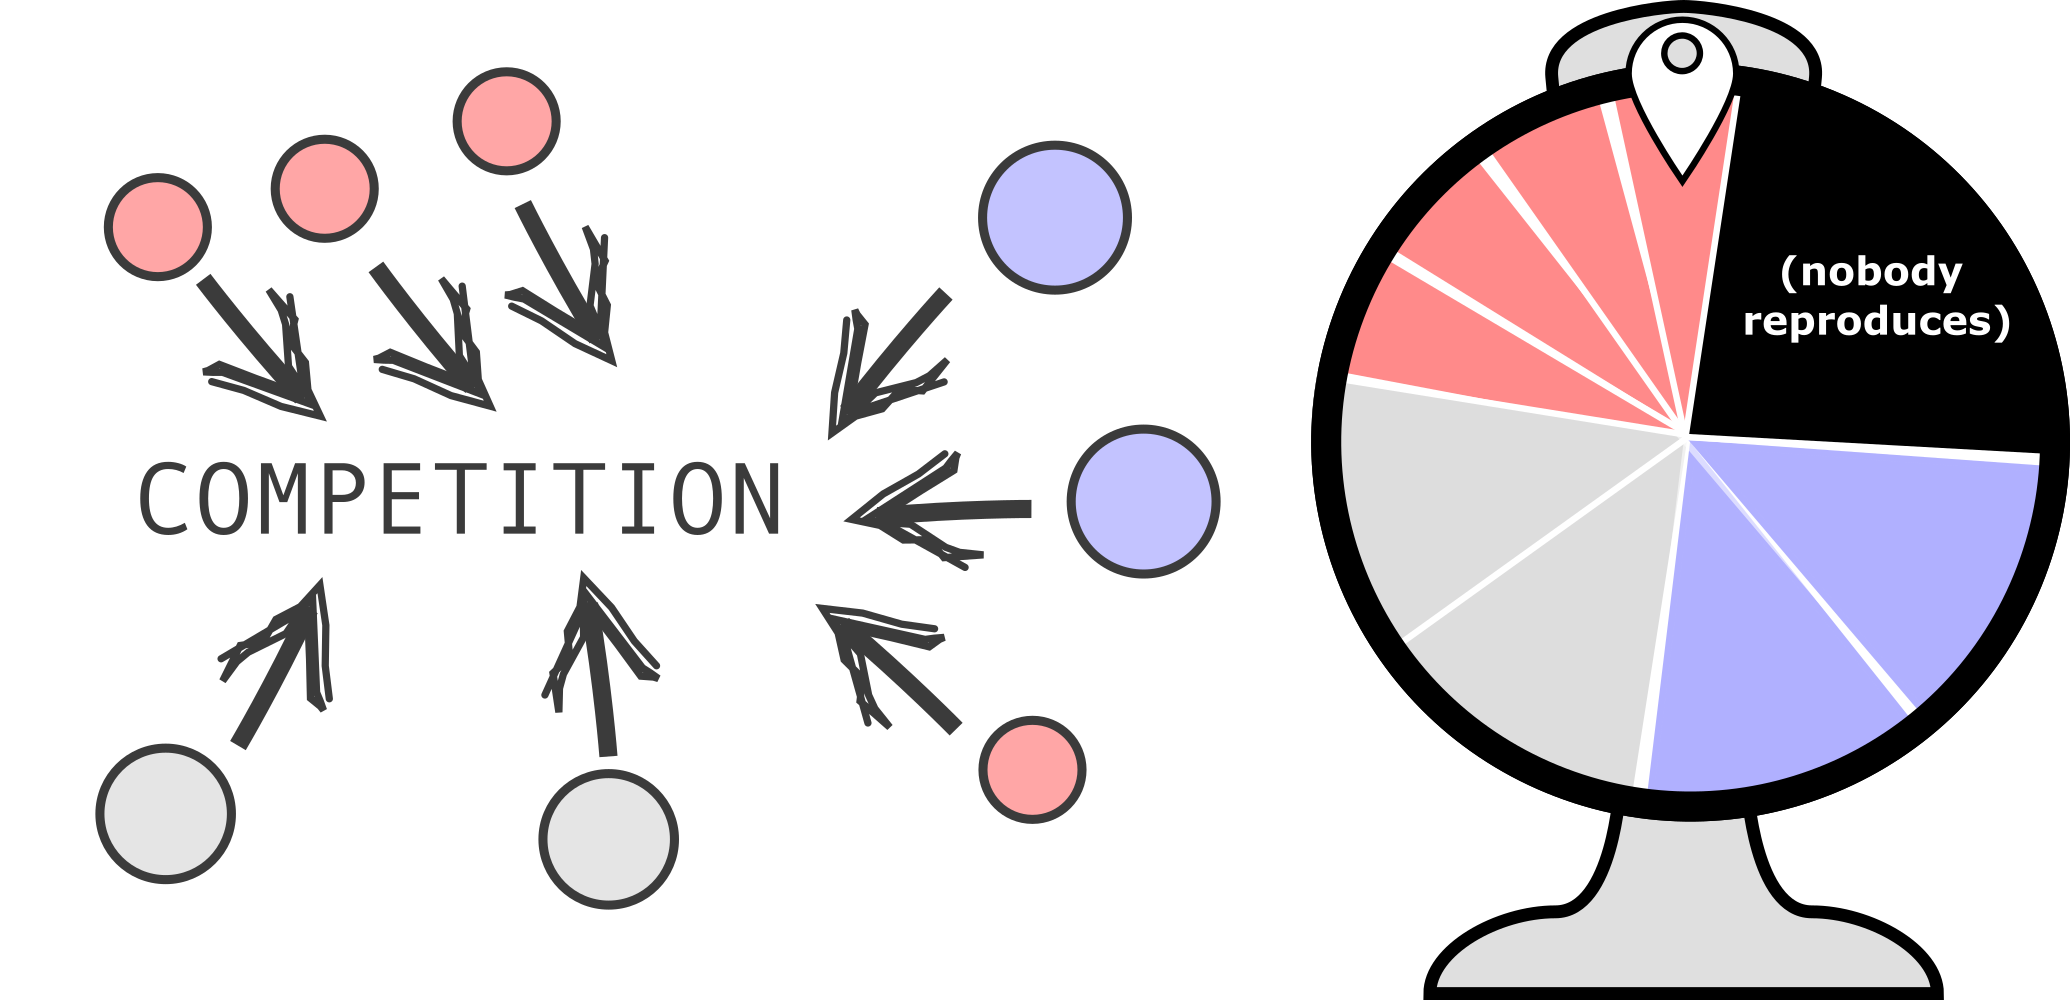
\includegraphics{images/roulette.png}

As can be seen, not all individual have the same size on the roulette
wheel. That depicts differences in their growth rates, biomass, or other
approximations of ``fitness''. Also, the roulette wheel contains an area
(shown in black) that shapes the chance that nobody reproduces. We will
try and implement this rule to let individuals reproduce based on their
fitness, but with only 10 competitors at a time. Let's start with a code
where individuals have a ``fitness'' value, but it not yet used for
selection (see below). \textbf{Read/test this code thoroughly before you
move on to the next section}.

\begin{tcolorbox}[enhanced jigsaw, leftrule=.75mm, colbacktitle=quarto-callout-note-color!10!white, coltitle=black, colback=white, left=2mm, bottomtitle=1mm, arc=.35mm, titlerule=0mm, breakable, bottomrule=.15mm, opacitybacktitle=0.6, colframe=quarto-callout-note-color-frame, title=\textcolor{quarto-callout-note-color}{\faInfo}\hspace{0.5em}{CODE FOR ``fitness without fitness''}, opacityback=0, toprule=.15mm, toptitle=1mm, rightrule=.15mm]

\begin{Shaded}
\begin{Highlighting}[]
\ImportTok{import}\NormalTok{ random}
\ImportTok{import}\NormalTok{ math}
\ImportTok{import}\NormalTok{ matplotlib.pyplot }\ImportTok{as}\NormalTok{ plt}

\CommentTok{\# Set the random number seed for reproducibility}
\NormalTok{random.seed(}\DecValTok{0}\NormalTok{)}

\NormalTok{plt.ion()  }\CommentTok{\# Enable interactive plotting}

\CommentTok{\# {-}{-}{-} PARAMETERS {-}{-}{-}}
\NormalTok{initial\_fitness }\OperatorTok{=} \FloatTok{0.1}            \CommentTok{\# Starting fitness for all individuals}
\NormalTok{population\_size }\OperatorTok{=} \DecValTok{500}             \CommentTok{\# Number of individuals (should be a square number for grid mode)}
\NormalTok{generations }\OperatorTok{=} \DecValTok{20000}               \CommentTok{\# Number of generations to simulate}
\NormalTok{mutation\_rate }\OperatorTok{=} \FloatTok{0.005}            \CommentTok{\# Probability of mutation per reproduction event}
\NormalTok{sample\_interval }\OperatorTok{=} \DecValTok{5}               \CommentTok{\# How often to sample and plot data}

\CommentTok{\# {-}{-}{-} INITIALIZATION {-}{-}{-}}
\CommentTok{\# Create initial population: all individuals start with the same fitness}
\NormalTok{population }\OperatorTok{=}\NormalTok{ [initial\_fitness }\ControlFlowTok{for}\NormalTok{ \_ }\KeywordTok{in} \BuiltInTok{range}\NormalTok{(population\_size)]}

\CommentTok{\# Lists to track average fitness and diversity over time}
\NormalTok{avg\_fitness }\OperatorTok{=}\NormalTok{ []}
\NormalTok{diversity\_over\_time }\OperatorTok{=}\NormalTok{ []}

\CommentTok{\# {-}{-}{-} CORE FUNCTIONS {-}{-}{-}}

\KeywordTok{def}\NormalTok{ mutate(fitness, rate}\OperatorTok{=}\NormalTok{mutation\_rate):}
    \CommentTok{"""Mutate the fitness value with a given probability."""}
    \ControlFlowTok{if}\NormalTok{ random.random() }\OperatorTok{\textless{}}\NormalTok{ rate:}
        \CommentTok{\# Fitness changes by a random value in [{-}0.1, 0.1], clipped to [0, 1]}
        \ControlFlowTok{return} \BuiltInTok{min}\NormalTok{(}\FloatTok{1.0}\NormalTok{, }\BuiltInTok{max}\NormalTok{(}\FloatTok{0.0}\NormalTok{, fitness }\OperatorTok{+}\NormalTok{ random.uniform(}\OperatorTok{{-}}\FloatTok{0.1}\NormalTok{, }\FloatTok{0.1}\NormalTok{)))}
    \ControlFlowTok{return}\NormalTok{ fitness}

\KeywordTok{def}\NormalTok{ calculate\_diversity(population):}
    \CommentTok{"""NOT YET IMPLEMENTED! Calculate diversity as the standard deviation of fitness values."""}
    \ControlFlowTok{return} \DecValTok{0} 

\CommentTok{\# {-}{-}{-} PLOTTING SETUP {-}{-}{-}}
\NormalTok{fig, ax1 }\OperatorTok{=}\NormalTok{ plt.subplots(figsize}\OperatorTok{=}\NormalTok{(}\DecValTok{12}\NormalTok{, }\DecValTok{8}\NormalTok{))}
\NormalTok{ax1.set\_xlabel(}\StringTok{"Generation"}\NormalTok{)}
\NormalTok{ax1.set\_ylabel(}\StringTok{"Average Fitness"}\NormalTok{, color}\OperatorTok{=}\StringTok{\textquotesingle{}tab:blue\textquotesingle{}}\NormalTok{)}
\NormalTok{ax1.set\_ylim(}\DecValTok{0}\NormalTok{, }\DecValTok{1}\NormalTok{)}
\NormalTok{line1, }\OperatorTok{=}\NormalTok{ ax1.plot([], [], color}\OperatorTok{=}\StringTok{\textquotesingle{}tab:blue\textquotesingle{}}\NormalTok{, linewidth}\OperatorTok{=}\DecValTok{2}\NormalTok{, label}\OperatorTok{=}\StringTok{\textquotesingle{}Fitness\textquotesingle{}}\NormalTok{)}
\NormalTok{ax1.tick\_params(axis}\OperatorTok{=}\StringTok{\textquotesingle{}y\textquotesingle{}}\NormalTok{, labelcolor}\OperatorTok{=}\StringTok{\textquotesingle{}tab:blue\textquotesingle{}}\NormalTok{)}

\CommentTok{\# Second y{-}axis for diversity}
\NormalTok{ax2 }\OperatorTok{=}\NormalTok{ ax1.twinx()}
\NormalTok{ax2.set\_ylabel(}\StringTok{"Diversity"}\NormalTok{, color}\OperatorTok{=}\StringTok{\textquotesingle{}tab:green\textquotesingle{}}\NormalTok{)}
\NormalTok{line2, }\OperatorTok{=}\NormalTok{ ax2.plot([], [], color}\OperatorTok{=}\StringTok{\textquotesingle{}tab:green\textquotesingle{}}\NormalTok{, linestyle}\OperatorTok{=}\StringTok{\textquotesingle{}:\textquotesingle{}}\NormalTok{, linewidth}\OperatorTok{=}\DecValTok{2}\NormalTok{, label}\OperatorTok{=}\StringTok{\textquotesingle{}Diversity\textquotesingle{}}\NormalTok{)}
\NormalTok{ax2.tick\_params(axis}\OperatorTok{=}\StringTok{\textquotesingle{}y\textquotesingle{}}\NormalTok{, labelcolor}\OperatorTok{=}\StringTok{\textquotesingle{}tab:green\textquotesingle{}}\NormalTok{)}

\NormalTok{fig.suptitle(}\StringTok{"Evolution Toward Fitness 1"}\NormalTok{)}
\NormalTok{fig.tight\_layout()}
\NormalTok{fig.legend(loc}\OperatorTok{=}\StringTok{\textquotesingle{}upper right\textquotesingle{}}\NormalTok{)}
\NormalTok{plt.grid(}\VariableTok{True}\NormalTok{)}
\NormalTok{plt.draw()}

\CommentTok{\# {-}{-}{-} EVOLUTION LOOP {-}{-}{-}}
\NormalTok{best\_fitness }\OperatorTok{=} \OperatorTok{{-}}\DecValTok{1}
\NormalTok{found }\OperatorTok{=} \VariableTok{False}

\ControlFlowTok{for}\NormalTok{ gen }\KeywordTok{in} \BuiltInTok{range}\NormalTok{(generations):}
\NormalTok{    total\_fit }\OperatorTok{=} \BuiltInTok{sum}\NormalTok{(population)}
\NormalTok{    best }\OperatorTok{=} \BuiltInTok{max}\NormalTok{(population)}
    \CommentTok{\# Print when a perfect solution is found}
    \ControlFlowTok{if}\NormalTok{ best }\OperatorTok{==} \DecValTok{1} \KeywordTok{and} \KeywordTok{not}\NormalTok{ found:}
\NormalTok{        found }\OperatorTok{=} \VariableTok{True}
        \BuiltInTok{print}\NormalTok{(}\StringTok{"Found perfect solution at generation"}\NormalTok{, gen)}
        
    \CommentTok{\# Sample and plot data at intervals}
    \ControlFlowTok{if}\NormalTok{ gen }\OperatorTok{\%}\NormalTok{ sample\_interval }\OperatorTok{==} \DecValTok{0}\NormalTok{:}
\NormalTok{        avg\_fitness.append(total\_fit }\OperatorTok{/}\NormalTok{ population\_size)}
\NormalTok{        diversity\_over\_time.append(calculate\_diversity(population))}
\NormalTok{        x\_vals }\OperatorTok{=}\NormalTok{ [i }\OperatorTok{*}\NormalTok{ sample\_interval }\ControlFlowTok{for}\NormalTok{ i }\KeywordTok{in} \BuiltInTok{range}\NormalTok{(}\BuiltInTok{len}\NormalTok{(avg\_fitness))]}
\NormalTok{        line1.set\_data(x\_vals, avg\_fitness)}
\NormalTok{        line2.set\_data(x\_vals, diversity\_over\_time)}
\NormalTok{        ax1.relim()}\OperatorTok{;}\NormalTok{ ax1.autoscale\_view()}
\NormalTok{        ax2.relim()}\OperatorTok{;}\NormalTok{ ax2.autoscale\_view()}
\NormalTok{        fig.suptitle(}\SpecialStringTok{f"Best Fitness: }\SpecialCharTok{\{}\NormalTok{best}\SpecialCharTok{:.2f\}}\SpecialStringTok{"}\NormalTok{, fontsize}\OperatorTok{=}\DecValTok{14}\NormalTok{)}
\NormalTok{        plt.pause(}\FloatTok{0.01}\NormalTok{)}
        

    \CommentTok{\# {-}{-}{-} MORAN PROCESS {-}{-}{-}}
    \CommentTok{\# For each individual, perform a reproduction event}
    \ControlFlowTok{for}\NormalTok{ \_ }\KeywordTok{in} \BuiltInTok{range}\NormalTok{(}\DecValTok{100}\NormalTok{):  }\CommentTok{\# 100 competition events per generation}
        \CommentTok{\# Select 1 random individual for replication}
\NormalTok{        probs }\OperatorTok{=}\NormalTok{ [}\DecValTok{1} \ControlFlowTok{for}\NormalTok{ fit }\KeywordTok{in}\NormalTok{ population] }\CommentTok{\# All probability weights are equal (1.0)}
\NormalTok{        parent\_idx }\OperatorTok{=}\NormalTok{ random.choices(}\BuiltInTok{range}\NormalTok{(}\BuiltInTok{len}\NormalTok{(population)), weights}\OperatorTok{=}\NormalTok{probs)[}\DecValTok{0}\NormalTok{] }\CommentTok{\# Grab one random individual based on an unweighted list...}
        \CommentTok{\# Select individual to be replaced (uniform random)}
\NormalTok{        dead\_idx }\OperatorTok{=}\NormalTok{ random.randrange(}\BuiltInTok{len}\NormalTok{(population))}
        \CommentTok{\# Copy population for next generation}
\NormalTok{        new\_pop }\OperatorTok{=}\NormalTok{ population.copy()}
        \CommentTok{\# Offspring replaces the dead individual (with possible mutation)}
\NormalTok{        new\_pop[dead\_idx] }\OperatorTok{=}\NormalTok{ mutate(population[parent\_idx])}
\NormalTok{        population }\OperatorTok{=}\NormalTok{ new\_pop}

\BuiltInTok{input}\NormalTok{(}\StringTok{"}\CharTok{\textbackslash{}n}\StringTok{Simulation complete. Press Enter to exit plot window..."}\NormalTok{)}
\end{Highlighting}
\end{Shaded}

\end{tcolorbox}

\section{Making a roulette wheel with everyone in
it}\label{making-a-roulette-wheel-with-everyone-in-it}

If you have read the code, you will see that we can pass a list of
weights to the function \texttt{random.choices}, to determine who is
most likely to be sampled. Currently, all the weights are set to 1:

\texttt{probs\ =\ {[}1\ for\ fit\ in\ population{]}\ \#\ All\ probability\ weights\ are\ equal\ (1.0)}

\begin{enumerate}
\def\labelenumi{\alph{enumi}.}
\tightlist
\item
  Run the code with the current (all equal) weights. What happens?
\item
  Modify this line of code to take the fitness values as the weight,
  rather than 1. (hint: this is a VERY small change in the code).
\end{enumerate}

\section{A roulette wheel of a subset of
individuals}\label{a-roulette-wheel-of-a-subset-of-individuals}

Instead of letting everyone reproduce, let us modify the code to only
sample from a smaller list of `competitors', and spin a virtual roulette
wheel to determine who wins. There are many ways to implement this, but
here's how we will do it. We will sample N individuals from the
population, and implement the following algorithm:

\begin{enumerate}
\def\labelenumi{\arabic{enumi}.}
\tightlist
\item
  Select a random subset of N individuals from the population.
\item
  Take/compute the fitness of each selected individual.
\item
  Add a reproduction-skip option with a fixed weight.
\item
  Choose one individual or the skip option using weighted random
  selection.
\item
  If an individual was chosen, mutate it and replace a random individual
  in the population.
\end{enumerate}

Below, there's a small snippet of code doing what is explained
above\footnote{Note that this is from the full code, so this code does
  not work stand-alone}. The variable \texttt{no\_reproduction\_chance}
is the fixed weight that nobody gets to reproduce:

\begin{tcolorbox}[enhanced jigsaw, leftrule=.75mm, colbacktitle=quarto-callout-note-color!10!white, coltitle=black, colback=white, left=2mm, bottomtitle=1mm, arc=.35mm, titlerule=0mm, breakable, bottomrule=.15mm, opacitybacktitle=0.6, colframe=quarto-callout-note-color-frame, title=\textcolor{quarto-callout-note-color}{\faInfo}\hspace{0.5em}{Roulette wheel algorithm}, opacityback=0, toprule=.15mm, toptitle=1mm, rightrule=.15mm]

\begin{Shaded}
\begin{Highlighting}[]
\NormalTok{  tournament\_size }\OperatorTok{=} \DecValTok{10}  
\NormalTok{  no\_reproduction\_chance }\OperatorTok{=} \DecValTok{1}
  
\NormalTok{  competitors }\OperatorTok{=}\NormalTok{ random.sample(population, tournament\_size)}
  \CommentTok{\# Make a list of their fitness values}
\NormalTok{  fitness\_values }\OperatorTok{=}\NormalTok{ [fit }\ControlFlowTok{for}\NormalTok{ fit }\KeywordTok{in}\NormalTok{ competitors]}
\NormalTok{  total }\OperatorTok{=} \BuiltInTok{sum}\NormalTok{(fitness\_values)}
  \CommentTok{\# Add a "no reproduction" dummy competitor with fitness = 0}
\NormalTok{  competitors\_with\_dummy }\OperatorTok{=}\NormalTok{ competitors }\OperatorTok{+}\NormalTok{ [}\VariableTok{None}\NormalTok{]}
\NormalTok{  probs }\OperatorTok{=}\NormalTok{ [f }\OperatorTok{/}\NormalTok{ total }\ControlFlowTok{for}\NormalTok{ f }\KeywordTok{in}\NormalTok{ fitness\_values] }\OperatorTok{+}\NormalTok{ [no\_reproduction\_chance]}
\NormalTok{  winner }\OperatorTok{=}\NormalTok{ random.choices(competitors\_with\_dummy, weights}\OperatorTok{=}\NormalTok{probs, k}\OperatorTok{=}\DecValTok{1}\NormalTok{)[}\DecValTok{0}\NormalTok{]}
  \ControlFlowTok{if}\NormalTok{ winner }\KeywordTok{is} \KeywordTok{not} \VariableTok{None}\NormalTok{:}
      \CommentTok{\# Mutate winner to produce offspring}
\NormalTok{      offspring }\OperatorTok{=}\NormalTok{ mutate(winner)}
\NormalTok{      remove\_idx }\OperatorTok{=}\NormalTok{ random.randrange(}\BuiltInTok{len}\NormalTok{(population))}
\NormalTok{      population[remove\_idx] }\OperatorTok{=}\NormalTok{ offspring  }
        
\end{Highlighting}
\end{Shaded}

\end{tcolorbox}

After you understand the roulette wheel algorithm, do the following
exercise:

\begin{exercise}[Questions about the roulette
wheel]\protect\hypertarget{exr-roulette}{}\label{exr-roulette}

\begin{enumerate}
\def\labelenumi{\alph{enumi}.}
\tightlist
\item
  Let's imagine a moment where the roulette wheel contains only 10
  highly unfit individuals (e.g.~all fitness values are 0.01). What is
  the chance that someone will reproduce? (you don't have to calculate
  it, but give your reasoning)
\item
  Answer the same question as in \textbf{a.}, but now imagine that all
  10 individuals have a fitness value of 1.
\item
  Answer question b. and c.~again, but now assume that
  \texttt{no\_reproduction\_chance} is equal to 0.
\item
  Describe what the \texttt{no\_reproduction\_chance} parameter does in
  biological terms.
\item
  Spatially structured populations are often placed on a grid.
  \textbf{Describe} how you could implement a roulette wheel to resolve
  \emph{local} competition, \emph{e.g.} when an empty grid point is
  competed for by the neighbours.
\end{enumerate}

\end{exercise}

\section{Diversity patterns}\label{diversity-patterns}

Modify the function \texttt{calculate\_diversity} to calculate the
diversity of the population as the standard deviation of the fitness
values.

\begin{exercise}[Questions about the roulette
wheel]\protect\hypertarget{exr-diversitydynamics}{}\label{exr-diversitydynamics}

\begin{enumerate}
\def\labelenumi{\alph{enumi}.}
\tightlist
\item
  Use a low mutation rate and study the dynamics of diversity. Describe
  the pattern verbally.
\end{enumerate}

\end{exercise}

\section{Evolving a DNA sequence}\label{evolving-a-dna-sequence}

A big problem with the previous model is there is no true distinction
between genotype (that which mutates) and phenotype (that which is
selected). Let us try and adapt the model to be more biologically
meaningful, by making each individual represented by a DNA sequence.
Copy the following code:

\begin{tcolorbox}[enhanced jigsaw, leftrule=.75mm, colbacktitle=quarto-callout-note-color!10!white, coltitle=black, colback=white, left=2mm, bottomtitle=1mm, arc=.35mm, titlerule=0mm, breakable, bottomrule=.15mm, opacitybacktitle=0.6, colframe=quarto-callout-note-color-frame, title=\textcolor{quarto-callout-note-color}{\faInfo}\hspace{0.5em}{Starting code for ``evolving a DNA sequence''}, opacityback=0, toprule=.15mm, toptitle=1mm, rightrule=.15mm]

\begin{Shaded}
\begin{Highlighting}[]
\ImportTok{import}\NormalTok{ random}
\ImportTok{import}\NormalTok{ math}
\ImportTok{import}\NormalTok{ matplotlib.pyplot }\ImportTok{as}\NormalTok{ plt}
\ImportTok{from}\NormalTok{ collections }\ImportTok{import}\NormalTok{ Counter}

\CommentTok{\# set the random number seed}
\NormalTok{random.seed(}\DecValTok{0}\NormalTok{)}

\NormalTok{plt.ion()  }\CommentTok{\# Enable interactive mode}

\CommentTok{\# Parameters}
\NormalTok{alphabet }\OperatorTok{=} \StringTok{"ATCG"}
\NormalTok{target\_sequence }\OperatorTok{=} \StringTok{"GATGCGCGCTGGATTAAC"}  \CommentTok{\# Example target sequence}
\NormalTok{dna\_length }\OperatorTok{=} \BuiltInTok{len}\NormalTok{(target\_sequence)}
\NormalTok{target\_length }\OperatorTok{=} \BuiltInTok{len}\NormalTok{(target\_sequence)}

\CommentTok{\# Simulation settings}
\NormalTok{population\_size }\OperatorTok{=} \DecValTok{500}  \CommentTok{\# must be a square number for grid mode}
\NormalTok{generations }\OperatorTok{=} \DecValTok{20000}
\NormalTok{mutation\_rate }\OperatorTok{=} \FloatTok{0.001}
\NormalTok{sample\_interval }\OperatorTok{=} \DecValTok{5}
\NormalTok{sample\_size }\OperatorTok{=}\NormalTok{ population\_size}
\NormalTok{no\_reproduction\_chance }\OperatorTok{=} \FloatTok{0.1}

\CommentTok{\# Core functions}
\KeywordTok{def}\NormalTok{ fitness(dna):}
    \ControlFlowTok{return} \DecValTok{1} \OperatorTok{{-}} \BuiltInTok{sum}\NormalTok{(a }\OperatorTok{!=}\NormalTok{ b }\ControlFlowTok{for}\NormalTok{ a, b }\KeywordTok{in} \BuiltInTok{zip}\NormalTok{(dna, target\_sequence)) }\OperatorTok{/}\NormalTok{ target\_length}

\KeywordTok{def}\NormalTok{ mutate(dna, rate}\OperatorTok{=}\NormalTok{mutation\_rate):}
    \ControlFlowTok{return} \StringTok{\textquotesingle{}\textquotesingle{}}\NormalTok{.join(}
\NormalTok{        random.choice([b }\ControlFlowTok{for}\NormalTok{ b }\KeywordTok{in}\NormalTok{ alphabet }\ControlFlowTok{if}\NormalTok{ b }\OperatorTok{!=}\NormalTok{ base]) }\ControlFlowTok{if}\NormalTok{ random.random() }\OperatorTok{\textless{}}\NormalTok{ rate }\ControlFlowTok{else}\NormalTok{ base}
        \ControlFlowTok{for}\NormalTok{ base }\KeywordTok{in}\NormalTok{ dna}
\NormalTok{    )}

\KeywordTok{def}\NormalTok{ count\_beneficial\_mutations(dna):}
\NormalTok{    f0 }\OperatorTok{=}\NormalTok{ fitness(dna)}
\NormalTok{    count }\OperatorTok{=} \DecValTok{0}
    \ControlFlowTok{for}\NormalTok{ i }\KeywordTok{in} \BuiltInTok{range}\NormalTok{(}\BuiltInTok{len}\NormalTok{(dna)):}
        \ControlFlowTok{for}\NormalTok{ b }\KeywordTok{in}\NormalTok{ alphabet:}
            \ControlFlowTok{if}\NormalTok{ b }\OperatorTok{!=}\NormalTok{ dna[i]:}
\NormalTok{                mutant }\OperatorTok{=}\NormalTok{ dna[:i] }\OperatorTok{+}\NormalTok{ b }\OperatorTok{+}\NormalTok{ dna[i}\OperatorTok{+}\DecValTok{1}\NormalTok{:]}
                \ControlFlowTok{if}\NormalTok{ fitness(mutant) }\OperatorTok{\textgreater{}}\NormalTok{ f0:}
\NormalTok{                    count }\OperatorTok{+=} \DecValTok{1}
    \ControlFlowTok{return}\NormalTok{ count}

\KeywordTok{def}\NormalTok{ diversity(pop):}
\NormalTok{    counts }\OperatorTok{=}\NormalTok{ \{\}}
    \ControlFlowTok{for}\NormalTok{ ind }\KeywordTok{in}\NormalTok{ pop:}
\NormalTok{        counts[ind] }\OperatorTok{=}\NormalTok{ counts.get(ind, }\DecValTok{0}\NormalTok{) }\OperatorTok{+} \DecValTok{1}
\NormalTok{    total }\OperatorTok{=} \BuiltInTok{len}\NormalTok{(pop)}
    \ControlFlowTok{return} \OperatorTok{{-}}\BuiltInTok{sum}\NormalTok{((c}\OperatorTok{/}\NormalTok{total) }\OperatorTok{*}\NormalTok{ math.log(c}\OperatorTok{/}\NormalTok{total }\OperatorTok{+} \FloatTok{1e{-}9}\NormalTok{) }\ControlFlowTok{for}\NormalTok{ c }\KeywordTok{in}\NormalTok{ counts.values()) }\ControlFlowTok{if}\NormalTok{ total }\OperatorTok{\textgreater{}} \DecValTok{0} \ControlFlowTok{else} \DecValTok{0}

\CommentTok{\# Initialize population}
\NormalTok{initial\_sequence }\OperatorTok{=} \StringTok{"GATAGCGAAGTTTAGCCG"} \CommentTok{\# far from target (only first 3 are correct)}
\NormalTok{population }\OperatorTok{=}\NormalTok{ [initial\_sequence }\ControlFlowTok{for}\NormalTok{ \_ }\KeywordTok{in} \BuiltInTok{range}\NormalTok{(population\_size)]}

\NormalTok{avg\_fitness }\OperatorTok{=}\NormalTok{ []}
\NormalTok{avg\_beneficial }\OperatorTok{=}\NormalTok{ []}
\NormalTok{diversity\_over\_time }\OperatorTok{=}\NormalTok{ []}
\NormalTok{best\_individuals }\OperatorTok{=}\NormalTok{ []}

\KeywordTok{def}\NormalTok{ get\_neighbors(i, j):}
    \ControlFlowTok{return}\NormalTok{ [(x }\OperatorTok{\%}\NormalTok{ side, y }\OperatorTok{\%}\NormalTok{ side)}
            \ControlFlowTok{for}\NormalTok{ x }\KeywordTok{in} \BuiltInTok{range}\NormalTok{(i}\OperatorTok{{-}}\DecValTok{1}\NormalTok{, i}\OperatorTok{+}\DecValTok{2}\NormalTok{)}
            \ControlFlowTok{for}\NormalTok{ y }\KeywordTok{in} \BuiltInTok{range}\NormalTok{(j}\OperatorTok{{-}}\DecValTok{1}\NormalTok{, j}\OperatorTok{+}\DecValTok{2}\NormalTok{)]}

\CommentTok{\# Initialize interactive plot}
\NormalTok{fig, ax1 }\OperatorTok{=}\NormalTok{ plt.subplots(figsize}\OperatorTok{=}\NormalTok{(}\DecValTok{12}\NormalTok{, }\DecValTok{8}\NormalTok{))}
\NormalTok{ax1.set\_xlabel(}\StringTok{"Generation"}\NormalTok{)}
\NormalTok{ax1.set\_ylabel(}\StringTok{"Average Fitness"}\NormalTok{, color}\OperatorTok{=}\StringTok{\textquotesingle{}tab:blue\textquotesingle{}}\NormalTok{)}
\NormalTok{ax1.set\_ylim(}\DecValTok{0}\NormalTok{, }\DecValTok{1}\NormalTok{)}
\NormalTok{line1, }\OperatorTok{=}\NormalTok{ ax1.plot([], [], color}\OperatorTok{=}\StringTok{\textquotesingle{}tab:blue\textquotesingle{}}\NormalTok{, linewidth}\OperatorTok{=}\DecValTok{2}\NormalTok{, label}\OperatorTok{=}\StringTok{\textquotesingle{}Fitness\textquotesingle{}}\NormalTok{)}
\NormalTok{ax1.tick\_params(axis}\OperatorTok{=}\StringTok{\textquotesingle{}y\textquotesingle{}}\NormalTok{, labelcolor}\OperatorTok{=}\StringTok{\textquotesingle{}tab:blue\textquotesingle{}}\NormalTok{)}

\NormalTok{ax2 }\OperatorTok{=}\NormalTok{ ax1.twinx()}
\NormalTok{ax2.set\_ylabel(}\StringTok{"Beneficial Mutations / Diversity"}\NormalTok{, color}\OperatorTok{=}\StringTok{\textquotesingle{}tab:purple\textquotesingle{}}\NormalTok{)}
\NormalTok{line2, }\OperatorTok{=}\NormalTok{ ax2.plot([], [], color}\OperatorTok{=}\StringTok{\textquotesingle{}tab:purple\textquotesingle{}}\NormalTok{, linestyle}\OperatorTok{=}\StringTok{\textquotesingle{}{-}{-}\textquotesingle{}}\NormalTok{, linewidth}\OperatorTok{=}\DecValTok{2}\NormalTok{, label}\OperatorTok{=}\StringTok{\textquotesingle{}Beneficial Mutations\textquotesingle{}}\NormalTok{)}
\NormalTok{line3, }\OperatorTok{=}\NormalTok{ ax2.plot([], [], color}\OperatorTok{=}\StringTok{\textquotesingle{}tab:green\textquotesingle{}}\NormalTok{, linestyle}\OperatorTok{=}\StringTok{\textquotesingle{}:\textquotesingle{}}\NormalTok{, linewidth}\OperatorTok{=}\DecValTok{2}\NormalTok{, label}\OperatorTok{=}\StringTok{\textquotesingle{}Diversity\textquotesingle{}}\NormalTok{)}
\NormalTok{ax2.tick\_params(axis}\OperatorTok{=}\StringTok{\textquotesingle{}y\textquotesingle{}}\NormalTok{, labelcolor}\OperatorTok{=}\StringTok{\textquotesingle{}tab:purple\textquotesingle{}}\NormalTok{)}
\NormalTok{fig.suptitle(}\StringTok{"Evolution Toward Target Sequence"}\NormalTok{)}
\NormalTok{fig.tight\_layout()}
\NormalTok{ax2.set\_ylim(}\DecValTok{0}\NormalTok{, }\DecValTok{20}\NormalTok{)}
\NormalTok{fig.legend(loc}\OperatorTok{=}\StringTok{\textquotesingle{}upper right\textquotesingle{}}\NormalTok{)}
\NormalTok{plt.grid(}\VariableTok{True}\NormalTok{)}
\NormalTok{plt.draw()}

\NormalTok{best\_seq }\OperatorTok{=} \StringTok{""}
\NormalTok{best\_score }\OperatorTok{=} \OperatorTok{{-}}\DecValTok{1}
\NormalTok{found }\OperatorTok{=} \VariableTok{False}

\CommentTok{\# Evolution loop}
\ControlFlowTok{for}\NormalTok{ gen }\KeywordTok{in} \BuiltInTok{range}\NormalTok{(generations):}
\NormalTok{    fitnesses }\OperatorTok{=}\NormalTok{ [fitness(ind) }\ControlFlowTok{for}\NormalTok{ ind }\KeywordTok{in}\NormalTok{ population]}
\NormalTok{    total\_fit }\OperatorTok{=} \BuiltInTok{sum}\NormalTok{(fitnesses)}
\NormalTok{    best }\OperatorTok{=} \BuiltInTok{max}\NormalTok{(fitnesses)}
    \ControlFlowTok{if}\NormalTok{(best }\OperatorTok{==} \DecValTok{1} \KeywordTok{and} \KeywordTok{not}\NormalTok{ found):}
\NormalTok{        found }\OperatorTok{=} \VariableTok{True}
        \BuiltInTok{print}\NormalTok{(}\StringTok{"Found perfect solution at generation"}\NormalTok{, gen)}
        
    \ControlFlowTok{if}\NormalTok{ gen }\OperatorTok{\%}\NormalTok{ sample\_interval }\OperatorTok{==} \DecValTok{0}\NormalTok{:}
\NormalTok{        sample }\OperatorTok{=}\NormalTok{ random.sample(population, sample\_size)}
\NormalTok{        avg\_beneficial.append(}\BuiltInTok{sum}\NormalTok{(count\_beneficial\_mutations(ind) }\ControlFlowTok{for}\NormalTok{ ind }\KeywordTok{in}\NormalTok{ sample) }\OperatorTok{/}\NormalTok{ sample\_size)}
\NormalTok{        diversity\_over\_time.append(diversity(population))}

        \CommentTok{\# Update plot data}
\NormalTok{        line1.set\_data(}\BuiltInTok{range}\NormalTok{(}\BuiltInTok{len}\NormalTok{(avg\_fitness)}\OperatorTok{+}\DecValTok{1}\NormalTok{), avg\_fitness }\OperatorTok{+}\NormalTok{ [}\BuiltInTok{sum}\NormalTok{(fitnesses)}\OperatorTok{/}\NormalTok{population\_size])}
\NormalTok{        line2.set\_data(}\BuiltInTok{range}\NormalTok{(}\BuiltInTok{len}\NormalTok{(avg\_beneficial)), avg\_beneficial)}
\NormalTok{        line3.set\_data(}\BuiltInTok{range}\NormalTok{(}\BuiltInTok{len}\NormalTok{(diversity\_over\_time)), diversity\_over\_time)}
\NormalTok{        ax1.relim()}\OperatorTok{;}\NormalTok{ ax1.autoscale\_view()}
\NormalTok{        ax2.relim()}\OperatorTok{;}\NormalTok{ ax2.autoscale\_view()}
\NormalTok{        best }\OperatorTok{=} \BuiltInTok{max}\NormalTok{(population, key}\OperatorTok{=}\NormalTok{fitness)}
\NormalTok{        fig.suptitle(}\SpecialStringTok{f"Best: }\SpecialCharTok{\{}\NormalTok{best}\SpecialCharTok{\}}\SpecialStringTok{ (target: }\SpecialCharTok{\{}\NormalTok{target\_sequence}\SpecialCharTok{\}}\SpecialStringTok{)"}\NormalTok{, fontsize}\OperatorTok{=}\DecValTok{14}\NormalTok{)}
\NormalTok{        plt.pause(}\FloatTok{0.01}\NormalTok{)}

    \ControlFlowTok{else}\NormalTok{:}
\NormalTok{        avg\_beneficial.append(avg\_beneficial[}\OperatorTok{{-}}\DecValTok{1}\NormalTok{])}
\NormalTok{        diversity\_over\_time.append(diversity\_over\_time[}\OperatorTok{{-}}\DecValTok{1}\NormalTok{])}

    \CommentTok{\# Tournament selection (as in evolving\_fitness\_final.py)}
\NormalTok{    new\_pop }\OperatorTok{=}\NormalTok{ []}
\NormalTok{    tournament\_size }\OperatorTok{=} \DecValTok{10}  \CommentTok{\# can be adjusted}

    \ControlFlowTok{for}\NormalTok{ \_ }\KeywordTok{in} \BuiltInTok{range}\NormalTok{(population\_size):}
        \CommentTok{\# Select tournament\_size individuals randomly}
\NormalTok{        competitors }\OperatorTok{=}\NormalTok{ random.sample(population, tournament\_size)}
        \CommentTok{\# Pick the one with highest fitness}
\NormalTok{        fitness\_values }\OperatorTok{=}\NormalTok{ [fitness(ind) }\ControlFlowTok{for}\NormalTok{ ind }\KeywordTok{in}\NormalTok{ competitors]}
\NormalTok{        total }\OperatorTok{=} \BuiltInTok{sum}\NormalTok{(fitness\_values)}
        
\NormalTok{        probs }\OperatorTok{=}\NormalTok{ [f }\OperatorTok{/}\NormalTok{ total }\ControlFlowTok{for}\NormalTok{ f }\KeywordTok{in}\NormalTok{ fitness\_values]}
\NormalTok{        winner }\OperatorTok{=}\NormalTok{ random.choices(competitors, weights}\OperatorTok{=}\NormalTok{probs, k}\OperatorTok{=}\DecValTok{1}\NormalTok{)[}\DecValTok{0}\NormalTok{]}
        \CommentTok{\# Mutate winner to produce offspring}
\NormalTok{        offspring }\OperatorTok{=}\NormalTok{ mutate(winner)}
\NormalTok{        new\_pop.append(offspring)}

\NormalTok{    population }\OperatorTok{=}\NormalTok{ new\_pop}

\NormalTok{    avg\_fitness.append(}\BuiltInTok{sum}\NormalTok{(fitness(ind) }\ControlFlowTok{for}\NormalTok{ ind }\KeywordTok{in}\NormalTok{ population) }\OperatorTok{/}\NormalTok{ population\_size)}
    \ControlFlowTok{if}\NormalTok{ gen }\OperatorTok{\%} \DecValTok{250} \OperatorTok{==} \DecValTok{0}\NormalTok{:}
\NormalTok{        best }\OperatorTok{=} \BuiltInTok{max}\NormalTok{(population, key}\OperatorTok{=}\NormalTok{fitness)}
\NormalTok{        best\_individuals.append((gen, best))}

\BuiltInTok{input}\NormalTok{(}\StringTok{"}\CharTok{\textbackslash{}n}\StringTok{Simulation complete. Press Enter to exit plot window..."}\NormalTok{)}
\end{Highlighting}
\end{Shaded}

\end{tcolorbox}

Answer the following questions using the options available in the model:

\begin{exercise}[Evolving
DNA]\protect\hypertarget{exr-evolving-dna}{}\label{exr-evolving-dna}

~

\begin{enumerate}
\def\labelenumi{\alph{enumi}.}
\tightlist
\item
  Run the code. What does the new (dashed blue) line represent? Do you
  understand how is changes over time?
\end{enumerate}

The program reports after how many generations it manages to find the
target sequence. With default settings this can take a long time\ldots{}
(default: 4633 generations)

\begin{enumerate}
\def\labelenumi{\alph{enumi}.}
\setcounter{enumi}{1}
\tightlist
\item
  Modify the mutation rate to see how it affects the time to find the
  target sequence. Try different mutation rates between 0.0001 and 0.1.
  Keep track of both how long (number of generations) it takes to find
  the target, and how fit the population is once the target is found.
  What do you observe?
\item
  Diversity is no longer calculated as the standard deviation in
  fitness, but as the Shannon diversity of all present sequences
  (although it is not super complex, you do not need to fully understand
  this function). Because of this, the exact number (quantities) cannot
  be compared to our ealrier model. Do you see a \emph{qualitative}
  differences?
\item
  Study how fitness is calculated in this model. Is there a distinction
  between genotype en phenotype? Why/why not?
\end{enumerate}

\end{exercise}

\section{Evolving a protein sequence}\label{evolving-a-protein-sequence}

Next we will extend the simulation a little more. The individual
genotypes will still be represented as a DNA sequence, but before
evaluating fitness this will be translated into a \textbf{protein}
sequence. To do so, the code first defines the codon table (which we of
course all know by heart =)), and then translates the DNA sequence into
a protein sequence. The protein sequence is then used to calculate the
fitness of the individual, which is based on how well the protein
sequence matches a target protein sequence. The code is as follows:

\begin{tcolorbox}[enhanced jigsaw, leftrule=.75mm, colbacktitle=quarto-callout-note-color!10!white, coltitle=black, colback=white, left=2mm, bottomtitle=1mm, arc=.35mm, titlerule=0mm, breakable, bottomrule=.15mm, opacitybacktitle=0.6, colframe=quarto-callout-note-color-frame, title=\textcolor{quarto-callout-note-color}{\faInfo}\hspace{0.5em}{Starting code for evolving a protein sequence}, opacityback=0, toprule=.15mm, toptitle=1mm, rightrule=.15mm]

\begin{Shaded}
\begin{Highlighting}[]
\ImportTok{import}\NormalTok{ random}
\ImportTok{import}\NormalTok{ math}
\ImportTok{import}\NormalTok{ matplotlib.pyplot }\ImportTok{as}\NormalTok{ plt}
\ImportTok{from}\NormalTok{ collections }\ImportTok{import}\NormalTok{ Counter}

\CommentTok{\# set the random number seed}
\NormalTok{random.seed(}\DecValTok{0}\NormalTok{)}

\NormalTok{plt.ion()  }\CommentTok{\# Enable interactive mode}

\CommentTok{\# Codon table}
\NormalTok{codon\_table }\OperatorTok{=}\NormalTok{ \{}
    \StringTok{\textquotesingle{}TTT\textquotesingle{}}\NormalTok{: }\StringTok{\textquotesingle{}F\textquotesingle{}}\NormalTok{, }\StringTok{\textquotesingle{}TTC\textquotesingle{}}\NormalTok{: }\StringTok{\textquotesingle{}F\textquotesingle{}}\NormalTok{, }\StringTok{\textquotesingle{}TTA\textquotesingle{}}\NormalTok{: }\StringTok{\textquotesingle{}L\textquotesingle{}}\NormalTok{, }\StringTok{\textquotesingle{}TTG\textquotesingle{}}\NormalTok{: }\StringTok{\textquotesingle{}L\textquotesingle{}}\NormalTok{, }\StringTok{\textquotesingle{}CTT\textquotesingle{}}\NormalTok{: }\StringTok{\textquotesingle{}L\textquotesingle{}}\NormalTok{, }\StringTok{\textquotesingle{}CTC\textquotesingle{}}\NormalTok{: }\StringTok{\textquotesingle{}L\textquotesingle{}}\NormalTok{, }\StringTok{\textquotesingle{}CTA\textquotesingle{}}\NormalTok{: }\StringTok{\textquotesingle{}L\textquotesingle{}}\NormalTok{, }\StringTok{\textquotesingle{}CTG\textquotesingle{}}\NormalTok{: }\StringTok{\textquotesingle{}L\textquotesingle{}}\NormalTok{,}
    \StringTok{\textquotesingle{}ATT\textquotesingle{}}\NormalTok{: }\StringTok{\textquotesingle{}I\textquotesingle{}}\NormalTok{, }\StringTok{\textquotesingle{}ATC\textquotesingle{}}\NormalTok{: }\StringTok{\textquotesingle{}I\textquotesingle{}}\NormalTok{, }\StringTok{\textquotesingle{}ATA\textquotesingle{}}\NormalTok{: }\StringTok{\textquotesingle{}I\textquotesingle{}}\NormalTok{, }\StringTok{\textquotesingle{}ATG\textquotesingle{}}\NormalTok{: }\StringTok{\textquotesingle{}M\textquotesingle{}}\NormalTok{,}
    \StringTok{\textquotesingle{}GTT\textquotesingle{}}\NormalTok{: }\StringTok{\textquotesingle{}V\textquotesingle{}}\NormalTok{, }\StringTok{\textquotesingle{}GTC\textquotesingle{}}\NormalTok{: }\StringTok{\textquotesingle{}V\textquotesingle{}}\NormalTok{, }\StringTok{\textquotesingle{}GTA\textquotesingle{}}\NormalTok{: }\StringTok{\textquotesingle{}V\textquotesingle{}}\NormalTok{, }\StringTok{\textquotesingle{}GTG\textquotesingle{}}\NormalTok{: }\StringTok{\textquotesingle{}V\textquotesingle{}}\NormalTok{,}
    \StringTok{\textquotesingle{}TCT\textquotesingle{}}\NormalTok{: }\StringTok{\textquotesingle{}S\textquotesingle{}}\NormalTok{, }\StringTok{\textquotesingle{}TCC\textquotesingle{}}\NormalTok{: }\StringTok{\textquotesingle{}S\textquotesingle{}}\NormalTok{, }\StringTok{\textquotesingle{}TCA\textquotesingle{}}\NormalTok{: }\StringTok{\textquotesingle{}S\textquotesingle{}}\NormalTok{, }\StringTok{\textquotesingle{}TCG\textquotesingle{}}\NormalTok{: }\StringTok{\textquotesingle{}S\textquotesingle{}}\NormalTok{, }\StringTok{\textquotesingle{}AGT\textquotesingle{}}\NormalTok{: }\StringTok{\textquotesingle{}S\textquotesingle{}}\NormalTok{, }\StringTok{\textquotesingle{}AGC\textquotesingle{}}\NormalTok{: }\StringTok{\textquotesingle{}S\textquotesingle{}}\NormalTok{,}
    \StringTok{\textquotesingle{}CCT\textquotesingle{}}\NormalTok{: }\StringTok{\textquotesingle{}P\textquotesingle{}}\NormalTok{, }\StringTok{\textquotesingle{}CCC\textquotesingle{}}\NormalTok{: }\StringTok{\textquotesingle{}P\textquotesingle{}}\NormalTok{, }\StringTok{\textquotesingle{}CCA\textquotesingle{}}\NormalTok{: }\StringTok{\textquotesingle{}P\textquotesingle{}}\NormalTok{, }\StringTok{\textquotesingle{}CCG\textquotesingle{}}\NormalTok{: }\StringTok{\textquotesingle{}P\textquotesingle{}}\NormalTok{,}
    \StringTok{\textquotesingle{}ACT\textquotesingle{}}\NormalTok{: }\StringTok{\textquotesingle{}T\textquotesingle{}}\NormalTok{, }\StringTok{\textquotesingle{}ACC\textquotesingle{}}\NormalTok{: }\StringTok{\textquotesingle{}T\textquotesingle{}}\NormalTok{, }\StringTok{\textquotesingle{}ACA\textquotesingle{}}\NormalTok{: }\StringTok{\textquotesingle{}T\textquotesingle{}}\NormalTok{, }\StringTok{\textquotesingle{}ACG\textquotesingle{}}\NormalTok{: }\StringTok{\textquotesingle{}T\textquotesingle{}}\NormalTok{,}
    \StringTok{\textquotesingle{}GCT\textquotesingle{}}\NormalTok{: }\StringTok{\textquotesingle{}A\textquotesingle{}}\NormalTok{, }\StringTok{\textquotesingle{}GCC\textquotesingle{}}\NormalTok{: }\StringTok{\textquotesingle{}A\textquotesingle{}}\NormalTok{, }\StringTok{\textquotesingle{}GCA\textquotesingle{}}\NormalTok{: }\StringTok{\textquotesingle{}A\textquotesingle{}}\NormalTok{, }\StringTok{\textquotesingle{}GCG\textquotesingle{}}\NormalTok{: }\StringTok{\textquotesingle{}A\textquotesingle{}}\NormalTok{,}
    \StringTok{\textquotesingle{}TAT\textquotesingle{}}\NormalTok{: }\StringTok{\textquotesingle{}Y\textquotesingle{}}\NormalTok{, }\StringTok{\textquotesingle{}TAC\textquotesingle{}}\NormalTok{: }\StringTok{\textquotesingle{}Y\textquotesingle{}}\NormalTok{, }\StringTok{\textquotesingle{}CAT\textquotesingle{}}\NormalTok{: }\StringTok{\textquotesingle{}H\textquotesingle{}}\NormalTok{, }\StringTok{\textquotesingle{}CAC\textquotesingle{}}\NormalTok{: }\StringTok{\textquotesingle{}H\textquotesingle{}}\NormalTok{,}
    \StringTok{\textquotesingle{}CAA\textquotesingle{}}\NormalTok{: }\StringTok{\textquotesingle{}Q\textquotesingle{}}\NormalTok{, }\StringTok{\textquotesingle{}CAG\textquotesingle{}}\NormalTok{: }\StringTok{\textquotesingle{}Q\textquotesingle{}}\NormalTok{, }\StringTok{\textquotesingle{}AAT\textquotesingle{}}\NormalTok{: }\StringTok{\textquotesingle{}N\textquotesingle{}}\NormalTok{, }\StringTok{\textquotesingle{}AAC\textquotesingle{}}\NormalTok{: }\StringTok{\textquotesingle{}N\textquotesingle{}}\NormalTok{,}
    \StringTok{\textquotesingle{}AAA\textquotesingle{}}\NormalTok{: }\StringTok{\textquotesingle{}K\textquotesingle{}}\NormalTok{, }\StringTok{\textquotesingle{}AAG\textquotesingle{}}\NormalTok{: }\StringTok{\textquotesingle{}K\textquotesingle{}}\NormalTok{, }\StringTok{\textquotesingle{}GAT\textquotesingle{}}\NormalTok{: }\StringTok{\textquotesingle{}D\textquotesingle{}}\NormalTok{, }\StringTok{\textquotesingle{}GAC\textquotesingle{}}\NormalTok{: }\StringTok{\textquotesingle{}D\textquotesingle{}}\NormalTok{,}
    \StringTok{\textquotesingle{}GAA\textquotesingle{}}\NormalTok{: }\StringTok{\textquotesingle{}E\textquotesingle{}}\NormalTok{, }\StringTok{\textquotesingle{}GAG\textquotesingle{}}\NormalTok{: }\StringTok{\textquotesingle{}E\textquotesingle{}}\NormalTok{, }\StringTok{\textquotesingle{}TGT\textquotesingle{}}\NormalTok{: }\StringTok{\textquotesingle{}C\textquotesingle{}}\NormalTok{, }\StringTok{\textquotesingle{}TGC\textquotesingle{}}\NormalTok{: }\StringTok{\textquotesingle{}C\textquotesingle{}}\NormalTok{,}
    \StringTok{\textquotesingle{}TGG\textquotesingle{}}\NormalTok{: }\StringTok{\textquotesingle{}W\textquotesingle{}}\NormalTok{, }\StringTok{\textquotesingle{}CGT\textquotesingle{}}\NormalTok{: }\StringTok{\textquotesingle{}R\textquotesingle{}}\NormalTok{, }\StringTok{\textquotesingle{}CGC\textquotesingle{}}\NormalTok{: }\StringTok{\textquotesingle{}R\textquotesingle{}}\NormalTok{, }\StringTok{\textquotesingle{}CGA\textquotesingle{}}\NormalTok{: }\StringTok{\textquotesingle{}R\textquotesingle{}}\NormalTok{, }\StringTok{\textquotesingle{}CGG\textquotesingle{}}\NormalTok{: }\StringTok{\textquotesingle{}R\textquotesingle{}}\NormalTok{, }\StringTok{\textquotesingle{}AGA\textquotesingle{}}\NormalTok{: }\StringTok{\textquotesingle{}R\textquotesingle{}}\NormalTok{, }\StringTok{\textquotesingle{}AGG\textquotesingle{}}\NormalTok{: }\StringTok{\textquotesingle{}R\textquotesingle{}}\NormalTok{,}
    \StringTok{\textquotesingle{}GGT\textquotesingle{}}\NormalTok{: }\StringTok{\textquotesingle{}G\textquotesingle{}}\NormalTok{, }\StringTok{\textquotesingle{}GGC\textquotesingle{}}\NormalTok{: }\StringTok{\textquotesingle{}G\textquotesingle{}}\NormalTok{, }\StringTok{\textquotesingle{}GGA\textquotesingle{}}\NormalTok{: }\StringTok{\textquotesingle{}G\textquotesingle{}}\NormalTok{, }\StringTok{\textquotesingle{}GGG\textquotesingle{}}\NormalTok{: }\StringTok{\textquotesingle{}G\textquotesingle{}}\NormalTok{,}
    \StringTok{\textquotesingle{}TAA\textquotesingle{}}\NormalTok{: }\StringTok{\textquotesingle{}*\textquotesingle{}}\NormalTok{, }\StringTok{\textquotesingle{}TAG\textquotesingle{}}\NormalTok{: }\StringTok{\textquotesingle{}*\textquotesingle{}}\NormalTok{, }\StringTok{\textquotesingle{}TGA\textquotesingle{}}\NormalTok{: }\StringTok{\textquotesingle{}*\textquotesingle{}}
\NormalTok{\}}

\CommentTok{\# Parameters}
\NormalTok{alphabet }\OperatorTok{=} \StringTok{"ATCG"}
\NormalTok{target\_protein }\OperatorTok{=} \StringTok{"DARWIN"}
\NormalTok{dna\_length }\OperatorTok{=} \BuiltInTok{len}\NormalTok{(target\_protein)}\OperatorTok{*}\DecValTok{3}
\NormalTok{target\_length }\OperatorTok{=} \BuiltInTok{len}\NormalTok{(target\_protein)}

\CommentTok{\# Simulation settings}
\NormalTok{population\_size }\OperatorTok{=} \DecValTok{625}  \CommentTok{\# must be a square number for grid mode}
\NormalTok{generations }\OperatorTok{=} \DecValTok{20000}
\NormalTok{mutation\_rate }\OperatorTok{=} \FloatTok{0.0005}   
\NormalTok{sample\_interval }\OperatorTok{=} \DecValTok{5}
\NormalTok{sample\_size }\OperatorTok{=}\NormalTok{ population\_size}
\NormalTok{no\_reproduction\_chance }\OperatorTok{=} \FloatTok{0.01}

\CommentTok{\# Core functions}
\KeywordTok{def}\NormalTok{ translate(dna):}
    \ControlFlowTok{return} \StringTok{\textquotesingle{}\textquotesingle{}}\NormalTok{.join(codon\_table.get(dna[i:i}\OperatorTok{+}\DecValTok{3}\NormalTok{], }\StringTok{\textquotesingle{}?\textquotesingle{}}\NormalTok{) }\ControlFlowTok{for}\NormalTok{ i }\KeywordTok{in} \BuiltInTok{range}\NormalTok{(}\DecValTok{0}\NormalTok{, }\BuiltInTok{len}\NormalTok{(dna), }\DecValTok{3}\NormalTok{))}

\KeywordTok{def}\NormalTok{ fitness(dna):}
\NormalTok{    protein }\OperatorTok{=}\NormalTok{ translate(dna)}
    \ControlFlowTok{return} \DecValTok{1} \OperatorTok{{-}} \BuiltInTok{sum}\NormalTok{(a }\OperatorTok{!=}\NormalTok{ b }\ControlFlowTok{for}\NormalTok{ a, b }\KeywordTok{in} \BuiltInTok{zip}\NormalTok{(protein, target\_protein)) }\OperatorTok{/}\NormalTok{ target\_length}

\KeywordTok{def}\NormalTok{ mutate(dna, rate}\OperatorTok{=}\NormalTok{mutation\_rate):}
    \ControlFlowTok{return} \StringTok{\textquotesingle{}\textquotesingle{}}\NormalTok{.join(}
\NormalTok{        random.choice([b }\ControlFlowTok{for}\NormalTok{ b }\KeywordTok{in}\NormalTok{ alphabet }\ControlFlowTok{if}\NormalTok{ b }\OperatorTok{!=}\NormalTok{ base]) }\ControlFlowTok{if}\NormalTok{ random.random() }\OperatorTok{\textless{}}\NormalTok{ rate }\ControlFlowTok{else}\NormalTok{ base}
        \ControlFlowTok{for}\NormalTok{ base }\KeywordTok{in}\NormalTok{ dna}
\NormalTok{    )}

\KeywordTok{def}\NormalTok{ count\_beneficial\_mutations(dna):}
\NormalTok{    f0 }\OperatorTok{=}\NormalTok{ fitness(dna)}
\NormalTok{    count }\OperatorTok{=} \DecValTok{0}
    \ControlFlowTok{for}\NormalTok{ i }\KeywordTok{in} \BuiltInTok{range}\NormalTok{(}\BuiltInTok{len}\NormalTok{(dna)):}
        \ControlFlowTok{for}\NormalTok{ b }\KeywordTok{in}\NormalTok{ alphabet:}
            \ControlFlowTok{if}\NormalTok{ b }\OperatorTok{!=}\NormalTok{ dna[i]:}
\NormalTok{                mutant }\OperatorTok{=}\NormalTok{ dna[:i] }\OperatorTok{+}\NormalTok{ b }\OperatorTok{+}\NormalTok{ dna[i}\OperatorTok{+}\DecValTok{1}\NormalTok{:]}
                \ControlFlowTok{if}\NormalTok{ fitness(mutant) }\OperatorTok{\textgreater{}}\NormalTok{ f0:}
\NormalTok{                    count }\OperatorTok{+=} \DecValTok{1}
    \ControlFlowTok{return}\NormalTok{ count}

\KeywordTok{def}\NormalTok{ diversity(pop):}
\NormalTok{    counts }\OperatorTok{=}\NormalTok{ Counter(pop)}
\NormalTok{    total }\OperatorTok{=} \BuiltInTok{len}\NormalTok{(pop)}
    \ControlFlowTok{return} \OperatorTok{{-}}\BuiltInTok{sum}\NormalTok{((c}\OperatorTok{/}\NormalTok{total) }\OperatorTok{*}\NormalTok{ math.log(c}\OperatorTok{/}\NormalTok{total }\OperatorTok{+} \FloatTok{1e{-}9}\NormalTok{) }\ControlFlowTok{for}\NormalTok{ c }\KeywordTok{in}\NormalTok{ counts.values()) }\ControlFlowTok{if}\NormalTok{ total }\OperatorTok{\textgreater{}} \DecValTok{0} \ControlFlowTok{else} \DecValTok{0}

\CommentTok{\# Initialize population}
\NormalTok{initial\_sequence }\OperatorTok{=} \StringTok{\textquotesingle{}\textquotesingle{}}\NormalTok{.join(random.choice(alphabet) }\ControlFlowTok{for}\NormalTok{ \_ }\KeywordTok{in} \BuiltInTok{range}\NormalTok{(dna\_length))}
\NormalTok{population }\OperatorTok{=}\NormalTok{ [initial\_sequence }\ControlFlowTok{for}\NormalTok{ \_ }\KeywordTok{in} \BuiltInTok{range}\NormalTok{(population\_size)]}

\NormalTok{avg\_fitness }\OperatorTok{=}\NormalTok{ []}
\NormalTok{avg\_beneficial }\OperatorTok{=}\NormalTok{ []}
\NormalTok{diversity\_over\_time }\OperatorTok{=}\NormalTok{ []}
\NormalTok{best\_individuals }\OperatorTok{=}\NormalTok{ []}

\CommentTok{\# Grid setup}
\NormalTok{side }\OperatorTok{=} \BuiltInTok{int}\NormalTok{(math.sqrt(population\_size))}
\ControlFlowTok{assert}\NormalTok{ side }\OperatorTok{*}\NormalTok{ side }\OperatorTok{==}\NormalTok{ population\_size, }\StringTok{"Population size must be a square number for grid mode"}

\KeywordTok{def}\NormalTok{ get\_neighbors(i, j):}
    \ControlFlowTok{return}\NormalTok{ [(x }\OperatorTok{\%}\NormalTok{ side, y }\OperatorTok{\%}\NormalTok{ side)}
            \ControlFlowTok{for}\NormalTok{ x }\KeywordTok{in} \BuiltInTok{range}\NormalTok{(i}\OperatorTok{{-}}\DecValTok{1}\NormalTok{, i}\OperatorTok{+}\DecValTok{2}\NormalTok{)}
            \ControlFlowTok{for}\NormalTok{ y }\KeywordTok{in} \BuiltInTok{range}\NormalTok{(j}\OperatorTok{{-}}\DecValTok{1}\NormalTok{, j}\OperatorTok{+}\DecValTok{2}\NormalTok{)]}

\CommentTok{\# Initialize interactive plot}
\NormalTok{fig, ax1 }\OperatorTok{=}\NormalTok{ plt.subplots(figsize}\OperatorTok{=}\NormalTok{(}\DecValTok{12}\NormalTok{, }\DecValTok{8}\NormalTok{))}
\NormalTok{ax1.set\_xlabel(}\StringTok{"Generation"}\NormalTok{)}
\NormalTok{ax1.set\_ylabel(}\StringTok{"Average Fitness"}\NormalTok{, color}\OperatorTok{=}\StringTok{\textquotesingle{}tab:blue\textquotesingle{}}\NormalTok{)}
\NormalTok{ax1.set\_ylim(}\DecValTok{0}\NormalTok{, }\DecValTok{1}\NormalTok{)}
\NormalTok{line0, }\OperatorTok{=}\NormalTok{ ax1.plot([], [], color}\OperatorTok{=}\StringTok{\textquotesingle{}black\textquotesingle{}}\NormalTok{, linewidth}\OperatorTok{=}\DecValTok{1}\NormalTok{, label}\OperatorTok{=}\StringTok{\textquotesingle{}Max fitness\textquotesingle{}}\NormalTok{)}
\NormalTok{line1, }\OperatorTok{=}\NormalTok{ ax1.plot([], [], color}\OperatorTok{=}\StringTok{\textquotesingle{}tab:blue\textquotesingle{}}\NormalTok{, linewidth}\OperatorTok{=}\DecValTok{2}\NormalTok{, label}\OperatorTok{=}\StringTok{\textquotesingle{}Fitness\textquotesingle{}}\NormalTok{)}
\NormalTok{ax1.tick\_params(axis}\OperatorTok{=}\StringTok{\textquotesingle{}y\textquotesingle{}}\NormalTok{, labelcolor}\OperatorTok{=}\StringTok{\textquotesingle{}tab:blue\textquotesingle{}}\NormalTok{)}

\NormalTok{ax2 }\OperatorTok{=}\NormalTok{ ax1.twinx()}
\NormalTok{ax2.set\_ylabel(}\StringTok{"Beneficial Mutations / Diversity"}\NormalTok{, color}\OperatorTok{=}\StringTok{\textquotesingle{}tab:purple\textquotesingle{}}\NormalTok{)}
\NormalTok{line2, }\OperatorTok{=}\NormalTok{ ax2.plot([], [], color}\OperatorTok{=}\StringTok{\textquotesingle{}tab:purple\textquotesingle{}}\NormalTok{, linestyle}\OperatorTok{=}\StringTok{\textquotesingle{}{-}{-}\textquotesingle{}}\NormalTok{, linewidth}\OperatorTok{=}\DecValTok{2}\NormalTok{, label}\OperatorTok{=}\StringTok{\textquotesingle{}Beneficial Mutations\textquotesingle{}}\NormalTok{)}
\NormalTok{line3, }\OperatorTok{=}\NormalTok{ ax2.plot([], [], color}\OperatorTok{=}\StringTok{\textquotesingle{}tab:green\textquotesingle{}}\NormalTok{, linestyle}\OperatorTok{=}\StringTok{\textquotesingle{}:\textquotesingle{}}\NormalTok{, linewidth}\OperatorTok{=}\DecValTok{2}\NormalTok{, label}\OperatorTok{=}\StringTok{\textquotesingle{}Diversity\textquotesingle{}}\NormalTok{)}
\NormalTok{ax2.tick\_params(axis}\OperatorTok{=}\StringTok{\textquotesingle{}y\textquotesingle{}}\NormalTok{, labelcolor}\OperatorTok{=}\StringTok{\textquotesingle{}tab:purple\textquotesingle{}}\NormalTok{)}
\NormalTok{fig.suptitle(}\StringTok{"Evolution Toward "} \OperatorTok{+} \BuiltInTok{str}\NormalTok{(target\_protein))}
\NormalTok{fig.tight\_layout()}
\NormalTok{ax2.set\_ylim(}\DecValTok{0}\NormalTok{, }\DecValTok{5}\NormalTok{)}
\NormalTok{fig.legend(loc}\OperatorTok{=}\StringTok{\textquotesingle{}upper right\textquotesingle{}}\NormalTok{)}
\NormalTok{plt.grid(}\VariableTok{True}\NormalTok{)}
\NormalTok{plt.draw()}

\NormalTok{best\_seq }\OperatorTok{=} \StringTok{""}
\NormalTok{best\_score }\OperatorTok{=} \OperatorTok{{-}}\DecValTok{1}
\NormalTok{best\_fitnesses }\OperatorTok{=}\NormalTok{ []}
\NormalTok{found }\OperatorTok{=} \VariableTok{False}

\CommentTok{\# Evolution loop}
\ControlFlowTok{for}\NormalTok{ gen }\KeywordTok{in} \BuiltInTok{range}\NormalTok{(generations):}
\NormalTok{    fitnesses }\OperatorTok{=}\NormalTok{ [fitness(ind) }\ControlFlowTok{for}\NormalTok{ ind }\KeywordTok{in}\NormalTok{ population]}
\NormalTok{    total\_fit }\OperatorTok{=} \BuiltInTok{sum}\NormalTok{(fitnesses)}
\NormalTok{    best }\OperatorTok{=} \BuiltInTok{max}\NormalTok{(fitnesses)}
\NormalTok{    best\_fitnesses.append(best)}
    \ControlFlowTok{if}\NormalTok{(best }\OperatorTok{==} \DecValTok{1} \KeywordTok{and} \KeywordTok{not}\NormalTok{ found):}
\NormalTok{        found }\OperatorTok{=} \VariableTok{True}
        \BuiltInTok{print}\NormalTok{(}\StringTok{"Found perfect solution at generation"}\NormalTok{, gen)}
        
    \ControlFlowTok{if}\NormalTok{ gen }\OperatorTok{\%}\NormalTok{ sample\_interval }\OperatorTok{==} \DecValTok{0}\NormalTok{:}
\NormalTok{        sample }\OperatorTok{=}\NormalTok{ random.sample(population, sample\_size)}
\NormalTok{        avg\_beneficial.append(}\BuiltInTok{sum}\NormalTok{(count\_beneficial\_mutations(ind) }\ControlFlowTok{for}\NormalTok{ ind }\KeywordTok{in}\NormalTok{ sample) }\OperatorTok{/}\NormalTok{ sample\_size)}
\NormalTok{        diversity\_over\_time.append(diversity(population))}

        \CommentTok{\# Update plot data}
\NormalTok{        line0.set\_data(}\BuiltInTok{range}\NormalTok{(}\BuiltInTok{len}\NormalTok{(avg\_fitness)}\OperatorTok{+}\DecValTok{1}\NormalTok{), best\_fitnesses)}
\NormalTok{        line1.set\_data(}\BuiltInTok{range}\NormalTok{(}\BuiltInTok{len}\NormalTok{(avg\_fitness)}\OperatorTok{+}\DecValTok{1}\NormalTok{), avg\_fitness }\OperatorTok{+}\NormalTok{ [}\BuiltInTok{sum}\NormalTok{(fitnesses)}\OperatorTok{/}\NormalTok{population\_size])}
\NormalTok{        line2.set\_data(}\BuiltInTok{range}\NormalTok{(}\BuiltInTok{len}\NormalTok{(avg\_beneficial)), avg\_beneficial)}
\NormalTok{        line3.set\_data(}\BuiltInTok{range}\NormalTok{(}\BuiltInTok{len}\NormalTok{(diversity\_over\_time)), diversity\_over\_time)}
\NormalTok{        ax1.relim()}\OperatorTok{;}\NormalTok{ ax1.autoscale\_view()}
\NormalTok{        ax2.relim()}\OperatorTok{;}\NormalTok{ ax2.autoscale\_view()}
\NormalTok{        best }\OperatorTok{=} \BuiltInTok{max}\NormalTok{(population, key}\OperatorTok{=}\NormalTok{fitness)}
\NormalTok{        fig.suptitle(}\SpecialStringTok{f"Best: }\SpecialCharTok{\{}\NormalTok{translate(best)}\SpecialCharTok{\}}\SpecialStringTok{ (target: }\SpecialCharTok{\{}\NormalTok{target\_protein}\SpecialCharTok{\}}\SpecialStringTok{)"}\NormalTok{, fontsize}\OperatorTok{=}\DecValTok{14}\NormalTok{)}
\NormalTok{        plt.pause(}\FloatTok{0.01}\NormalTok{)}

    \ControlFlowTok{else}\NormalTok{:}
\NormalTok{        avg\_beneficial.append(avg\_beneficial[}\OperatorTok{{-}}\DecValTok{1}\NormalTok{])}
\NormalTok{        diversity\_over\_time.append(diversity\_over\_time[}\OperatorTok{{-}}\DecValTok{1}\NormalTok{])}

\NormalTok{    new\_pop }\OperatorTok{=}\NormalTok{ []}
\NormalTok{    tournament\_size }\OperatorTok{=} \DecValTok{10}  \CommentTok{\# can be adjusted}
    
    \ControlFlowTok{for}\NormalTok{ \_ }\KeywordTok{in} \BuiltInTok{range}\NormalTok{(population\_size):}
        \CommentTok{\# Select tournament\_size individuals randomly}
\NormalTok{        competitors }\OperatorTok{=}\NormalTok{ random.sample(population, tournament\_size)}
        \CommentTok{\# Pick the one with highest fitness}
\NormalTok{        fitness\_values }\OperatorTok{=}\NormalTok{ [fitness(ind) }\ControlFlowTok{for}\NormalTok{ ind }\KeywordTok{in}\NormalTok{ competitors]}
\NormalTok{        total }\OperatorTok{=} \BuiltInTok{sum}\NormalTok{(fitness\_values)}
        
\NormalTok{        probs }\OperatorTok{=}\NormalTok{ [f }\OperatorTok{/}\NormalTok{ total }\ControlFlowTok{for}\NormalTok{ f }\KeywordTok{in}\NormalTok{ fitness\_values]}
\NormalTok{        winner }\OperatorTok{=}\NormalTok{ random.choices(competitors, weights}\OperatorTok{=}\NormalTok{probs, k}\OperatorTok{=}\DecValTok{1}\NormalTok{)[}\DecValTok{0}\NormalTok{]}
        \CommentTok{\# Mutate winner to produce offspring}
\NormalTok{        offspring }\OperatorTok{=}\NormalTok{ mutate(winner)}
\NormalTok{        new\_pop.append(offspring)}

\NormalTok{    population }\OperatorTok{=}\NormalTok{ new\_pop}


\NormalTok{    avg\_fitness.append(}\BuiltInTok{sum}\NormalTok{(fitness(ind) }\ControlFlowTok{for}\NormalTok{ ind }\KeywordTok{in}\NormalTok{ population) }\OperatorTok{/}\NormalTok{ population\_size)}
    \ControlFlowTok{if}\NormalTok{ gen }\OperatorTok{\%} \DecValTok{250} \OperatorTok{==} \DecValTok{0}\NormalTok{:}
\NormalTok{        best }\OperatorTok{=} \BuiltInTok{max}\NormalTok{(population, key}\OperatorTok{=}\NormalTok{fitness)}
\NormalTok{        best\_individuals.append((gen, translate(best)))}

\BuiltInTok{input}\NormalTok{(}\StringTok{"}\CharTok{\textbackslash{}n}\StringTok{Simulation complete. Press Enter to exit plot window..."}\NormalTok{)}
\end{Highlighting}
\end{Shaded}

\end{tcolorbox}

Answer the following question about the model:

\begin{exercise}[Evolving protein
sequences]\protect\hypertarget{exr-evolving-proteins}{}\label{exr-evolving-proteins}

~

\begin{enumerate}
\def\labelenumi{\alph{enumi}.}
\tightlist
\item
  Another line was added to the model. What new information can you
  obtain from analysing this line?
\item
  Study carefully how the other lines (also present in previous models)
  change over time. What do you observe? Try and capture what you see
  into words.
\item
  In biology, multiple genotypes can translate to the same phenotype
  (this is called a many-to-one genotype-phenotype map), or
  alternatively, one genotype can produce multiple phenotype (this is
  called phenotypic plasticity, or a one-to-many genotype-phenotype
  map). Which genotype-phenotype (GP) mapping applies to this model?
  Why?
\item
  \textbf{Bonus question for motivated students} modify the code to
  include a second target protein sequence, and alternate between the
  two targets. If you see something interesting, please share it with
  the class!
\end{enumerate}

\end{exercise}

\chapter{Practical 3}\label{practical-3-1}

\section{Building a model from
scratch}\label{building-a-model-from-scratch}

Over the last weeks you have been given many model of biology, and you
have modified or extended upon them. For this practical, I will give you
a only a description. Your challenge will be to see how far you get in
trying to get this model working yourself. I advice you use AI-assisted
programming only to solve small steps, otherwise you have no clue what
you are doing. But if you try and do everything yourself, it may take a
little long.

At the end of the pratical, we will compare different implementations by
students, as well as my implementation. Hopefully, we will see some
generic patterns, because the model description should be good enough to
give ``similar models''. The description should be ``vague enough'' to
lead to some differences, but ``precise enough'' to yield similar
results. This is an experiment in and of itself. So let's see :')

Note that I also do not yet know exactly what will happen in this
simulation (although I have tried it out), so I'm hoping we will learn
some cool stuff together!

\section{Simulating a simple microbial ecosystem with ``public
goods''}\label{simulating-a-simple-microbial-ecosystem-with-public-goods}

\subsection{Model description}\label{model-description}

Microbes often produce public goods, from which surrounding microbes can
benefit. This can lead to interesting dynamics, such as cooperation and
competition. Most models however consider on 1 public good at a time,
which leads to limited diversity (a producer, and a non-producer may or
may not coexist). Here, we will an ecosystem with many public goods, and
simulate them on a grid.

An individual microbe will carry a ``genome'' that is represented by a
binary string (101010010011). Each position in the string represents a
public good, and whether the individual can produce it (1) or not (0).
The individual can rely on other individuals to produce public goods.

We will simulate individuals (microbial cells) reproducing and dying on
a grid. A grid point either contains an individual, or it is empty.
Every empty point, will be competed for by individuals that are in that
neighbourhood. The neighbourhood is defined as the 8 surrounding grid
points (this is called the ``Moore'' neighbourhood). The cells can only
replicate if they have all the public goods they need, which means that
they can rely on other individuals in their neighbourhood to produce
them. If they do not have all public goods available, they cannot
replicate. The ``winner'' from these (max) 8 viable competitors will be
determined by a roulette wheel selection, where the relative probability
is determined by their fitness:

\[
F_i = 1 - c \cdot \sum({bitstring})
\]

In other words, fitness goes down as the number of public goods produced
increases, and there is a cost \(c\) associated with producing each
public good. Make sure this roulette wheel contains a probability that
nobody wins, such that highly unfit individuals are less likely to
replicate than highly fit individuals (also see earlier practicals).

The individual that replicates, can undergo mutations in the bitstring
(gene loss and gene gain). Assume gene loss is more likely than gene
gain (initial parameters to explore are summarised below)

Finally, implement a function that allows you to mix the grid (all
individuals are placed in a random position).

\subsection{Model output}\label{model-output}

The model will have the following output: a grid that is coloured by the
number of public goods produced (for consistency, let's all use a
`viridis' scale), and a line graph that plots the total population
sizes, as well as the population sizes of species producing 0 public
goods, 1 public good, 2 public goods, etc. (see
Figure~\ref{fig-examplegrid})

\subsection{Parameters to start out
with}\label{parameters-to-start-out-with}

\begin{itemize}
\tightlist
\item
  Grid size: 50 x 50
\item
  Initial population: produces all public goods (1111\ldots1)
\item
  Death rate: 0.1
\item
  Cost (c): 0.05
\item
  Bitstring 1 to 0 mutation (losing a gene): 0.01
\item
  Bitstring 0 to 1 mutation (gaining a gene): 0.001
\item
  Number of public goods (i.e.~bitstring length): 10
\item
  ``No-event'' size of roulette wheel: 1
\end{itemize}

\begin{figure}

\centering{

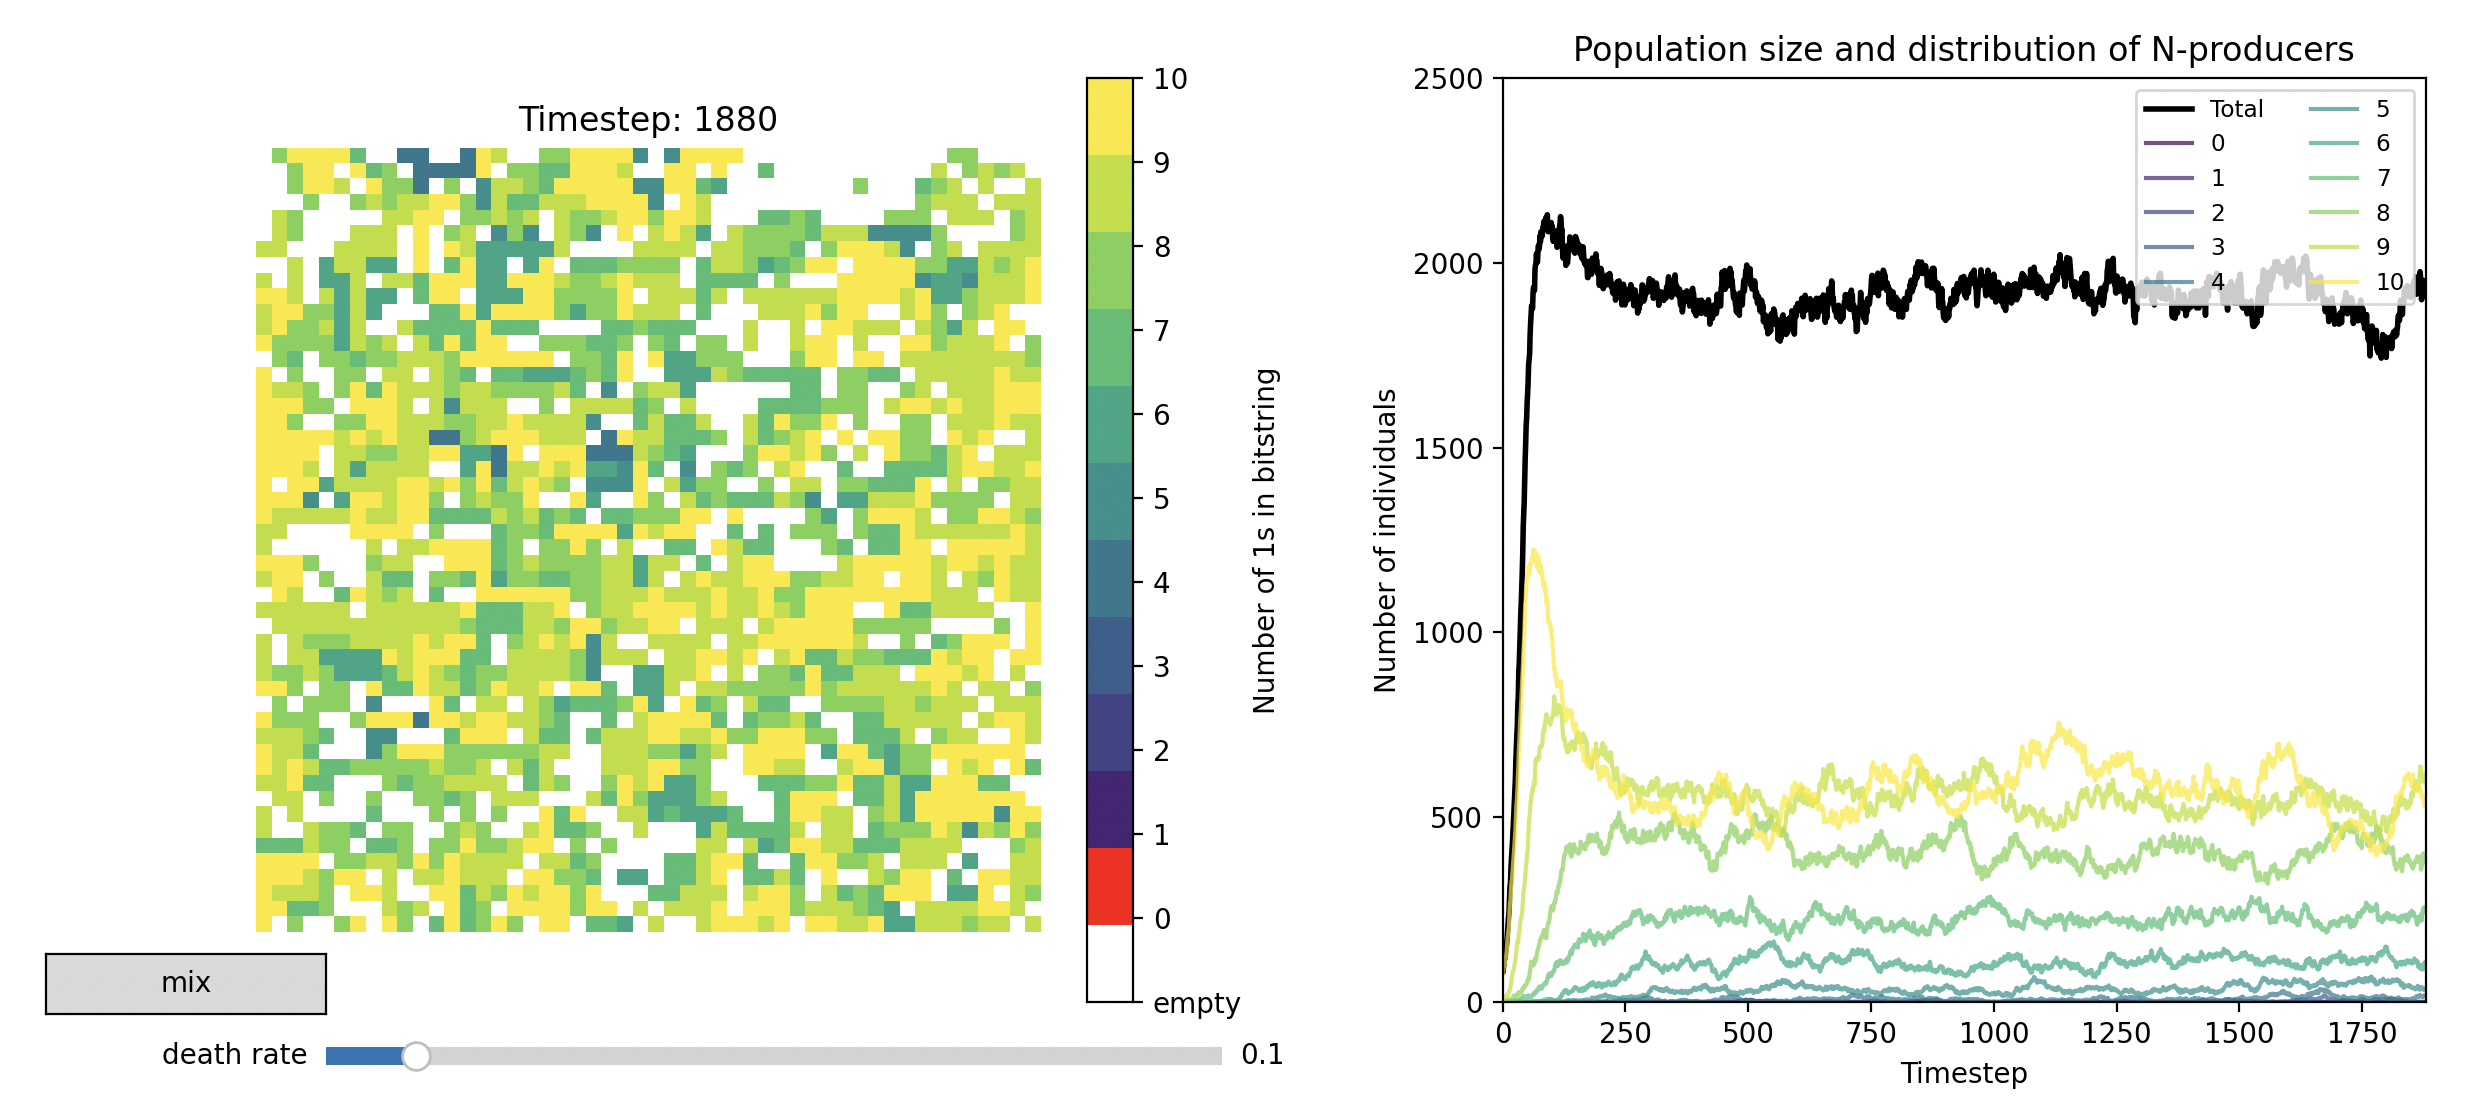
\includegraphics{images/evo_pract3_example.png}

}

\caption{\label{fig-examplegrid}Example of what the simulation could
look like}

\end{figure}%

\subsection{Proposed experiments}\label{proposed-experiments}

Try investigating how the model behaves with different values of \(c\)
(the cost of producing public goods). Can you explain what happens at
\(c=0.0\)?

Try studying the effect of mixing the whole grid every timestep, such
that neighbourhoods are constantly ``randomised''. Look at the
population size, as well as the distribution of different types. Can you
explain the observations in biological terms?

Try studying what happens at different mutation rates.

\chapter{Answers exercises}\label{answers-exercises}

\section{Answers to Evolution Practical
1}\label{answers-to-evolution-practical-1}

\subsection{\texorpdfstring{Questions
Exercise~\ref{exr-steering}}{Questions Exercise~}}\label{questions-exr-steering}

\begin{enumerate}
\def\labelenumi{\alph{enumi}.}
\item
  For this, you can simply multiply the velocity components every
  timestep by a value \textgreater{} 1. For example:

\begin{Shaded}
\begin{Highlighting}[]
\CommentTok{\# Accellerate the velocity}
\NormalTok{vx }\OperatorTok{*=} \FloatTok{1.01}
\NormalTok{vy }\OperatorTok{*=} \FloatTok{1.01}
\end{Highlighting}
\end{Shaded}

  Note that this gets out of hand quite quickly.
\item
  To do this, we need to store the new values in a temporary variable,
  and then assign them to the original variables. This is necessary
  because while we first modify vx, we still want to use the `old' value
  of vx to calculate the new vy. The following code rotates the velocity
  vector by 0.05 radians:

\begin{Shaded}
\begin{Highlighting}[]
\CommentTok{\# Rotate the velocity vector by a small angle }
\NormalTok{vxnew }\OperatorTok{=}\NormalTok{ vx }\OperatorTok{*}\NormalTok{ np.cos(}\FloatTok{0.05}\NormalTok{) }\OperatorTok{{-}}\NormalTok{ vy }\OperatorTok{*}\NormalTok{ np.sin(}\FloatTok{0.05}\NormalTok{)}
\NormalTok{vynew }\OperatorTok{=}\NormalTok{ vx }\OperatorTok{*}\NormalTok{ np.sin(}\FloatTok{0.05}\NormalTok{) }\OperatorTok{+}\NormalTok{ vy }\OperatorTok{*}\NormalTok{ np.cos(}\FloatTok{0.05}\NormalTok{)}
\NormalTok{vx, vy }\OperatorTok{=}\NormalTok{ vxnew, vynew}
\end{Highlighting}
\end{Shaded}

  If you run this code, you will see that the dot will go in circles.
\item
  While the code above stores x, y, vx, and vy as a `global variables',
  this is not good if we have many individuals. Instead, we can store
  the state of each individual in a list, dictionary, or a class. For
  example, we make a class `cell' and store 100 of these `cells' in a
  large list:

\begin{Shaded}
\begin{Highlighting}[]
\KeywordTok{class}\NormalTok{ Cell:}
    \KeywordTok{def} \FunctionTok{\_\_init\_\_}\NormalTok{(}\VariableTok{self}\NormalTok{, x, y, vx, vy):}
        \VariableTok{self}\NormalTok{.x }\OperatorTok{=}\NormalTok{ x}
        \VariableTok{self}\NormalTok{.y }\OperatorTok{=}\NormalTok{ y}
        \VariableTok{self}\NormalTok{.vx }\OperatorTok{=}\NormalTok{ vx}
        \VariableTok{self}\NormalTok{.vy }\OperatorTok{=}\NormalTok{ vy}

\CommentTok{\# Create 100 cells with random positions and 0 velocity}
\NormalTok{cells }\OperatorTok{=}\NormalTok{ [Cell(np.random.rand(), np.random.rand(), }\FloatTok{0.0}\NormalTok{, }\FloatTok{0.0}\NormalTok{) }\ControlFlowTok{for}\NormalTok{ \_ }\KeywordTok{in} \BuiltInTok{range}\NormalTok{(}\DecValTok{100}\NormalTok{)]}
\end{Highlighting}
\end{Shaded}
\end{enumerate}

\subsection{\texorpdfstring{Moving the target
(Section~\ref{sec-movingtarget})}{Moving the target (Section~)}}\label{moving-the-target-sec-movingtarget}

A working code to steer the individuals towards the target is shown
below. Note that the acceleration that is applied is only small,
otherwise the individuals will move in a straight line towards the
target very rapidly.

\begin{Shaded}
\begin{Highlighting}[]
\KeywordTok{def}\NormalTok{ move\_towards\_dot(}\VariableTok{self}\NormalTok{, cell):}
   \CommentTok{"""Apply forces in the direction of the dot."""}
   \CommentTok{\# Calculate dx and dy}
\NormalTok{   dx }\OperatorTok{=} \VariableTok{self}\NormalTok{.target\_position[}\DecValTok{0}\NormalTok{] }\OperatorTok{{-}}\NormalTok{ cell.x}
\NormalTok{   dy }\OperatorTok{=} \VariableTok{self}\NormalTok{.target\_position[}\DecValTok{1}\NormalTok{] }\OperatorTok{{-}}\NormalTok{ cell.y}
   \CommentTok{\# Calculate the distance to the target (pythagorean theorem)}
\NormalTok{   distance }\OperatorTok{=}\NormalTok{ np.sqrt(dx}\OperatorTok{**}\DecValTok{2} \OperatorTok{+}\NormalTok{ dy}\OperatorTok{**}\DecValTok{2}\NormalTok{)}
   
   \CommentTok{\# Normalize dx and dy }
\NormalTok{   dx }\OperatorTok{/=}\NormalTok{ distance}
\NormalTok{   dy }\OperatorTok{/=}\NormalTok{ distance}
   \CommentTok{\# Apply a small force towards the target}
\NormalTok{   cell.ax }\OperatorTok{+=}\NormalTok{ dx }\OperatorTok{*} \FloatTok{0.01}
\NormalTok{   cell.ay }\OperatorTok{+=}\NormalTok{ dy }\OperatorTok{*} \FloatTok{0.01}
\end{Highlighting}
\end{Shaded}

\subsection{\texorpdfstring{Reproduction
(Section~\ref{sec-reproduction})}{Reproduction (Section~)}}\label{reproduction-sec-reproduction}

A working code to reproduce a cell is shown below. Note that I decided
to first throw an individual away, and then add the newborn individual
(instead of the other way around). This ensures the newborn cannot be
immediately thrown away, which would be a rather pointless event.

\begin{Shaded}
\begin{Highlighting}[]
\KeywordTok{def}\NormalTok{ reproduce\_cell(}\VariableTok{self}\NormalTok{, cell):}
        \CommentTok{\# Reproduce: Create a new cell with the same properties as the current cell}
\NormalTok{        angle }\OperatorTok{=}\NormalTok{ np.random.uniform(}\DecValTok{0}\NormalTok{, }\DecValTok{2} \OperatorTok{*}\NormalTok{ np.pi)}
\NormalTok{        radius }\OperatorTok{=}\NormalTok{ np.random.uniform(}\FloatTok{0.05}\NormalTok{, }\FloatTok{1.5}\NormalTok{)}
\NormalTok{        new\_x }\OperatorTok{=}\NormalTok{ cell.x }\OperatorTok{+}\NormalTok{ radius }\OperatorTok{*}\NormalTok{ np.cos(angle)}
\NormalTok{        new\_y }\OperatorTok{=}\NormalTok{ cell.y }\OperatorTok{+}\NormalTok{ radius }\OperatorTok{*}\NormalTok{ np.sin(angle)}
\NormalTok{        new\_cell }\OperatorTok{=}\NormalTok{ Cell(new\_x, new\_y, cell.vx, cell.vy)}
\NormalTok{        random\_cell }\OperatorTok{=}\NormalTok{ np.random.choice(}\VariableTok{self}\NormalTok{.cells)   }
        \VariableTok{self}\NormalTok{.cells.remove(random\_cell)}
        \VariableTok{self}\NormalTok{.cells.append(new\_cell)}
\end{Highlighting}
\end{Shaded}

\subsection{\texorpdfstring{Collision
(Section~\ref{sec-collision})}{Collision (Section~)}}\label{collision-sec-collision}

A working code for cell-cell collision is shown below. Note that we
apply a large force as we want this force to be able to overpower other
forces that make the cells overlap.

\begin{Shaded}
\begin{Highlighting}[]
 \KeywordTok{def}\NormalTok{ avoid\_collision(}\VariableTok{self}\NormalTok{, cell):}
        \CommentTok{"""Avoidance forces to prevent cells from colliding."""}
        \ControlFlowTok{for}\NormalTok{ other\_cell }\KeywordTok{in} \VariableTok{self}\NormalTok{.cells:}
            \ControlFlowTok{if}\NormalTok{ other\_cell }\KeywordTok{is} \KeywordTok{not}\NormalTok{ cell:}
                \CommentTok{\# Calculate the distance between the two cells}
\NormalTok{                dx }\OperatorTok{=}\NormalTok{ cell.x }\OperatorTok{{-}}\NormalTok{ other\_cell.x}
\NormalTok{                dy }\OperatorTok{=}\NormalTok{ cell.y }\OperatorTok{{-}}\NormalTok{ other\_cell.y}
\NormalTok{                distance }\OperatorTok{=}\NormalTok{ np.sqrt(dx}\OperatorTok{**}\DecValTok{2} \OperatorTok{+}\NormalTok{ dy}\OperatorTok{**}\DecValTok{2}\NormalTok{)}

                \CommentTok{\# If the cells are too close, apply a repulsion force}
                \ControlFlowTok{if}\NormalTok{ distance }\OperatorTok{\textless{}} \FloatTok{5.0} \KeywordTok{and}\NormalTok{ distance }\OperatorTok{\textgreater{}} \DecValTok{0}\NormalTok{:  }\CommentTok{\# Threshold for "too close"}
                    \CommentTok{\# repulsion force proportional to the inverse of the distance}
\NormalTok{                    force\_magnitude }\OperatorTok{=}\NormalTok{ (}\FloatTok{5.0} \OperatorTok{{-}}\NormalTok{ distance) }\OperatorTok{/}\NormalTok{ distance}
\NormalTok{                    cell.ax }\OperatorTok{+=}\NormalTok{ force\_magnitude }\OperatorTok{*}\NormalTok{ dx  }\OperatorTok{*} \DecValTok{100}
\NormalTok{                    cell.ay }\OperatorTok{+=}\NormalTok{ force\_magnitude }\OperatorTok{*}\NormalTok{ dy }\OperatorTok{*} \DecValTok{100}
\end{Highlighting}
\end{Shaded}

\subsection{\texorpdfstring{A resource peak
(Section~\ref{sec-resourcepeak})}{A resource peak (Section~)}}\label{a-resource-peak-sec-resourcepeak}

A working code to implement a resource peak (with optional noise set to
0 by default) is shown below:

\begin{Shaded}
\begin{Highlighting}[]
\KeywordTok{def}\NormalTok{ fill\_grid(}\VariableTok{self}\NormalTok{, grid, mean\_x, mean\_y, std\_dev, noise}\OperatorTok{=}\DecValTok{0}\NormalTok{):}
        \CommentTok{"""Creates a Gaussian distribution with noise on the grid."""}
        \ControlFlowTok{for}\NormalTok{ i }\KeywordTok{in} \BuiltInTok{range}\NormalTok{(WORLD\_SIZE):}
            \ControlFlowTok{for}\NormalTok{ j }\KeywordTok{in} \BuiltInTok{range}\NormalTok{(WORLD\_SIZE):}
\NormalTok{                x }\OperatorTok{=}\NormalTok{ i }\OperatorTok{/}\NormalTok{ (WORLD\_SIZE }\OperatorTok{{-}} \DecValTok{1}\NormalTok{)}
\NormalTok{                y }\OperatorTok{=}\NormalTok{ j }\OperatorTok{/}\NormalTok{ (WORLD\_SIZE }\OperatorTok{{-}} \DecValTok{1}\NormalTok{)}
\NormalTok{                distance\_squared }\OperatorTok{=}\NormalTok{ (x }\OperatorTok{{-}}\NormalTok{ mean\_x)}\OperatorTok{**}\DecValTok{2} \OperatorTok{+}\NormalTok{ (y }\OperatorTok{{-}}\NormalTok{ mean\_y)}\OperatorTok{**}\DecValTok{2}
\NormalTok{                grid[i, j] }\OperatorTok{=}\NormalTok{ np.exp(}\OperatorTok{{-}}\NormalTok{distance\_squared }\OperatorTok{/}\NormalTok{ (}\DecValTok{2} \OperatorTok{*}\NormalTok{ std\_dev}\OperatorTok{**}\DecValTok{2}\NormalTok{)) }\OperatorTok{*}\NormalTok{ np.random.uniform(}\FloatTok{0.0}\NormalTok{, }\FloatTok{1.0}\NormalTok{)}\OperatorTok{**}\NormalTok{noise}

        \CommentTok{\# Normalize the grid to keep the total resource concentration the same}
\NormalTok{        grid }\OperatorTok{/=}\NormalTok{ np.}\BuiltInTok{sum}\NormalTok{(grid)}
        \VariableTok{self}\NormalTok{.grid }\OperatorTok{=}\NormalTok{ grid}
\end{Highlighting}
\end{Shaded}

\subsection{\texorpdfstring{Run and tumble
(Section~\ref{sec-runandtumble})}{Run and tumble (Section~)}}\label{run-and-tumble-sec-runandtumble}

A working code to implement a run-and-tumble mechanism shown below:

\begin{Shaded}
\begin{Highlighting}[]
\KeywordTok{def}\NormalTok{ find\_peak(}\VariableTok{self}\NormalTok{, cell):}
        \CommentTok{\# Convert cell position to grid indices, as well as the previous position}
\NormalTok{        grid\_x }\OperatorTok{=} \BuiltInTok{int}\NormalTok{(cell.x) }\OperatorTok{\%}\NormalTok{ WORLD\_SIZE}
\NormalTok{        grid\_y }\OperatorTok{=} \BuiltInTok{int}\NormalTok{(cell.y) }\OperatorTok{\%}\NormalTok{ WORLD\_SIZE}
\NormalTok{        next\_x }\OperatorTok{=}\NormalTok{ (}\BuiltInTok{int}\NormalTok{(cell.x }\OperatorTok{+} \DecValTok{10}\OperatorTok{*}\NormalTok{cell.vx) }\OperatorTok{+}\NormalTok{ WORLD\_SIZE) }\OperatorTok{\%}\NormalTok{ WORLD\_SIZE }
\NormalTok{        next\_y }\OperatorTok{=}\NormalTok{ (}\BuiltInTok{int}\NormalTok{(cell.y }\OperatorTok{+} \DecValTok{10}\OperatorTok{*}\NormalTok{cell.vy) }\OperatorTok{+}\NormalTok{ WORLD\_SIZE) }\OperatorTok{\%}\NormalTok{ WORLD\_SIZE }
        \CommentTok{\# Get the resource value at cell\textquotesingle{}s position, as well as the next position}
\NormalTok{        resource\_value }\OperatorTok{=} \VariableTok{self}\NormalTok{.grid[grid\_x, grid\_y]}
\NormalTok{        resource\_next }\OperatorTok{=} \VariableTok{self}\NormalTok{.grid[next\_x, next\_y]}
        
        \CommentTok{\# Check if the cell is moving in the right direction}
        \ControlFlowTok{if}\NormalTok{ resource\_next }\OperatorTok{\textgreater{}}\NormalTok{ resource\_value:}
            \CommentTok{\# Moving in the right direction: small random adjustment}
\NormalTok{            angle }\OperatorTok{=}\NormalTok{ np.random.uniform(}\OperatorTok{{-}}\FloatTok{0.1}\NormalTok{, }\FloatTok{0.1}\NormalTok{)  }\CommentTok{\# Small angle change}
        \ControlFlowTok{else}\NormalTok{:}
            \CommentTok{\# Moving in the wrong direction: large random adjustment}
\NormalTok{            angle }\OperatorTok{=}\NormalTok{ np.random.uniform(}\OperatorTok{{-}}\NormalTok{np.pi}\OperatorTok{*}\FloatTok{1.0}\NormalTok{, np.pi}\OperatorTok{*}\FloatTok{1.0}\NormalTok{)  }\CommentTok{\# Large angle change}
        
        \CommentTok{\# Rotate the velocity vector by the angle calculated}
\NormalTok{        new\_vx }\OperatorTok{=}\NormalTok{ cell.vx }\OperatorTok{*}\NormalTok{ np.cos(angle) }\OperatorTok{{-}}\NormalTok{ cell.vy }\OperatorTok{*}\NormalTok{ np.sin(angle)}
\NormalTok{        new\_vy }\OperatorTok{=}\NormalTok{ cell.vx }\OperatorTok{*}\NormalTok{ np.sin(angle) }\OperatorTok{+}\NormalTok{ cell.vy }\OperatorTok{*}\NormalTok{ np.cos(angle)}
    
        \CommentTok{\# Update the acceleration with the new velocity vector}
\NormalTok{        cell.vx }\OperatorTok{=}\NormalTok{ new\_vx}
\NormalTok{        cell.vy }\OperatorTok{=}\NormalTok{ new\_vy}
\NormalTok{        cell.ax }\OperatorTok{+=}\NormalTok{ cell.vx}
\NormalTok{        cell.ay }\OperatorTok{+=}\NormalTok{ cell.vy}
\end{Highlighting}
\end{Shaded}

\subsection{\texorpdfstring{Stickiness
(Section~\ref{sec-sticking})}{Stickiness (Section~)}}\label{stickiness-sec-sticking}

A working code for stickiness is shown below. The force applied here is
smaller than the collision force (as said, we want to try and avoid
collision even as cells want to move closer to eachother).

\begin{Shaded}
\begin{Highlighting}[]
\KeywordTok{def}\NormalTok{ stick\_to\_close(}\VariableTok{self}\NormalTok{, cell):}
        \CommentTok{"""Stick to closeby cells."""}
        \ControlFlowTok{for}\NormalTok{ other\_cell }\KeywordTok{in} \VariableTok{self}\NormalTok{.cells:}
            \ControlFlowTok{if}\NormalTok{ other\_cell }\KeywordTok{is} \KeywordTok{not}\NormalTok{ cell:}
                \CommentTok{\# Calculate the distance between the two cells}
\NormalTok{                dx }\OperatorTok{=}\NormalTok{ cell.x }\OperatorTok{{-}}\NormalTok{ other\_cell.x}
\NormalTok{                dy }\OperatorTok{=}\NormalTok{ cell.y }\OperatorTok{{-}}\NormalTok{ other\_cell.y}
\NormalTok{                distance }\OperatorTok{=}\NormalTok{ np.sqrt(dx}\OperatorTok{**}\DecValTok{2} \OperatorTok{+}\NormalTok{ dy}\OperatorTok{**}\DecValTok{2}\NormalTok{)}

                \CommentTok{\# If the cells are too close, apply a repulsion force}
                \ControlFlowTok{if}\NormalTok{ distance }\OperatorTok{\textless{}} \DecValTok{12} \KeywordTok{and}\NormalTok{ distance }\OperatorTok{\textgreater{}} \DecValTok{5}\NormalTok{:  }\CommentTok{\# Threshold for "close"}
                    \CommentTok{\# Calculate the repulsion force proportional to the inverse of the distance}
\NormalTok{                    cell.ax }\OperatorTok{{-}=}\NormalTok{ cell.stickiness }\OperatorTok{*}\NormalTok{ dx }\OperatorTok{*}\DecValTok{10}
\NormalTok{                    cell.ay }\OperatorTok{{-}=}\NormalTok{ cell.stickiness }\OperatorTok{*}\NormalTok{ dy }\OperatorTok{*}\DecValTok{10}
\end{Highlighting}
\end{Shaded}

\subsection{\texorpdfstring{The evolution of stickiness
(Exercise~\ref{exr-jsmodel})}{The evolution of stickiness (Exercise~)}}\label{the-evolution-of-stickiness-exr-jsmodel}

\begin{enumerate}
\def\labelenumi{\alph{enumi}.}
\tightlist
\item
  In the full model, stickiness naturally evolves to be higher. Natural
  selection therefore favours stickiness. However, it does not keep
  increasing and it stabilises around 0.25.
\item
  The \textbf{advantages} of stickiness are that larger groups of cells
  are better at steering towards the resources. Even if a single cell
  tries to go in the wrong direction, it will be pulled back. Together,
  they are less sensitive to the noise. Another distinct advantage is
  that the stickiest cells are sorted to be in the center of the group
  (as you have already seen earlier in this course!). That means that
  even after the peak was found, the stickiest cells have an advantage
  over the other cells as they can occupy the peak of the resource
  distribution. The \textbf{disadvantages} of stickiness are that larger
  groups move more slowly, and that the sticky clusters tend to stay
  together even if there are many resource peaks (and therewith miss out
  on resources).
\item
  The duration of the seasonal cycle is very important. If it is very
  long, it does not matter that the large clusters move slowly, as they
  will be better at finding and staying on the peak by being sticky. If
  the cycle is however very short, it may be more important to be able
  to move quickly and change direction rapidly. In that case, being too
  sticky may be a problem. As you modify this parameter in the online
  model, you will indeed see that shorter seasons mostly cause
  stickiness to drift close to 0.0, while longer seasons cause
  stickiness to evolve towards 0.25 or even higher.
\end{enumerate}

\section{Answers to Evolution Practical
2}\label{answers-to-evolution-practical-2}

\subsection{\texorpdfstring{Questions
Exercise~\ref{exr-roulette}}{Questions Exercise~}}\label{questions-exr-roulette}

\begin{enumerate}
\def\labelenumi{\alph{enumi}.}
\tightlist
\item
  If we sample 10 unfit individuals, the weight of the
  \texttt{no\_reproduction\_event} is proportionally high (the black
  slice of the roulette wheel is big). Hence, there is only a small
  chance that anyone will reproduce.
\item
  If we sample 10 fit individuals (fitness 1), the chances are much
  higher that someone will reproduce.
\item
  If the dummy value is 0, the chances that someone will reproduce are
  the same in both scenarios, as even with very unfit individuals there
  is no chance that nobody reproduces.
\item
  In nature, if no individual is sufficiently fit, reproduction may not
  occur at all. For example, if the competing individuals are bacteria
  with very low glucose uptake rates, they may not yet be
  physiologically ready to reproduce. In such cases, population size
  should remain stable or even decline if death is also occurring. The
  no\_reproduction\_event captures this by ensuring that fitness is not
  judged solely in relative terms against other individuals, but also in
  absolute terms against environmental demands.
\item
  If a grid point is empty (contains no individual), make a list of (up
  to) 8 individuals around that grid point. Apply the roulette wheel for
  those individuals, and place the `winner' inside the empty grid point.
\end{enumerate}

\subsection{\texorpdfstring{Questions
Exercise~\ref{exr-diversitydynamics}}{Questions Exercise~}}\label{questions-exr-diversitydynamics}

A snippet to calculate the standard deviation of a population is shown
below. Note that this value is already being plotted, so if you modify
this function you ought to be able to see what happens immediately.

\begin{Shaded}
\begin{Highlighting}[]
\KeywordTok{def}\NormalTok{ calculate\_diversity(population):}
    \CommentTok{"""Calculate diversity as the standard deviation of fitness values."""}
\NormalTok{    mean }\OperatorTok{=} \BuiltInTok{sum}\NormalTok{(population) }\OperatorTok{/} \BuiltInTok{len}\NormalTok{(population)}
\NormalTok{    variance }\OperatorTok{=} \BuiltInTok{sum}\NormalTok{((x }\OperatorTok{{-}}\NormalTok{ mean) }\OperatorTok{**} \DecValTok{2} \ControlFlowTok{for}\NormalTok{ x }\KeywordTok{in}\NormalTok{ population) }\OperatorTok{/}\NormalTok{ (}\BuiltInTok{len}\NormalTok{(population) }\OperatorTok{{-}} \DecValTok{1}\NormalTok{)}
    \ControlFlowTok{return}\NormalTok{ math.sqrt(variance)}
\end{Highlighting}
\end{Shaded}

\begin{enumerate}
\def\labelenumi{\alph{enumi}.}
\tightlist
\item
  The green dotted line is the standard deviation of the values in the
  population (`diversity'). From this we can see that the population is
  only breifly diverse whenever a new, fit individual appears. In
  between these phases, diversity is 0. This makes intuitive
  (biological) sense, as with a low mutation rate the only moments where
  there is more than 1 species is during the invasion of a new mutant.
  During all other phases, there is just a single (fittest) species.
\end{enumerate}

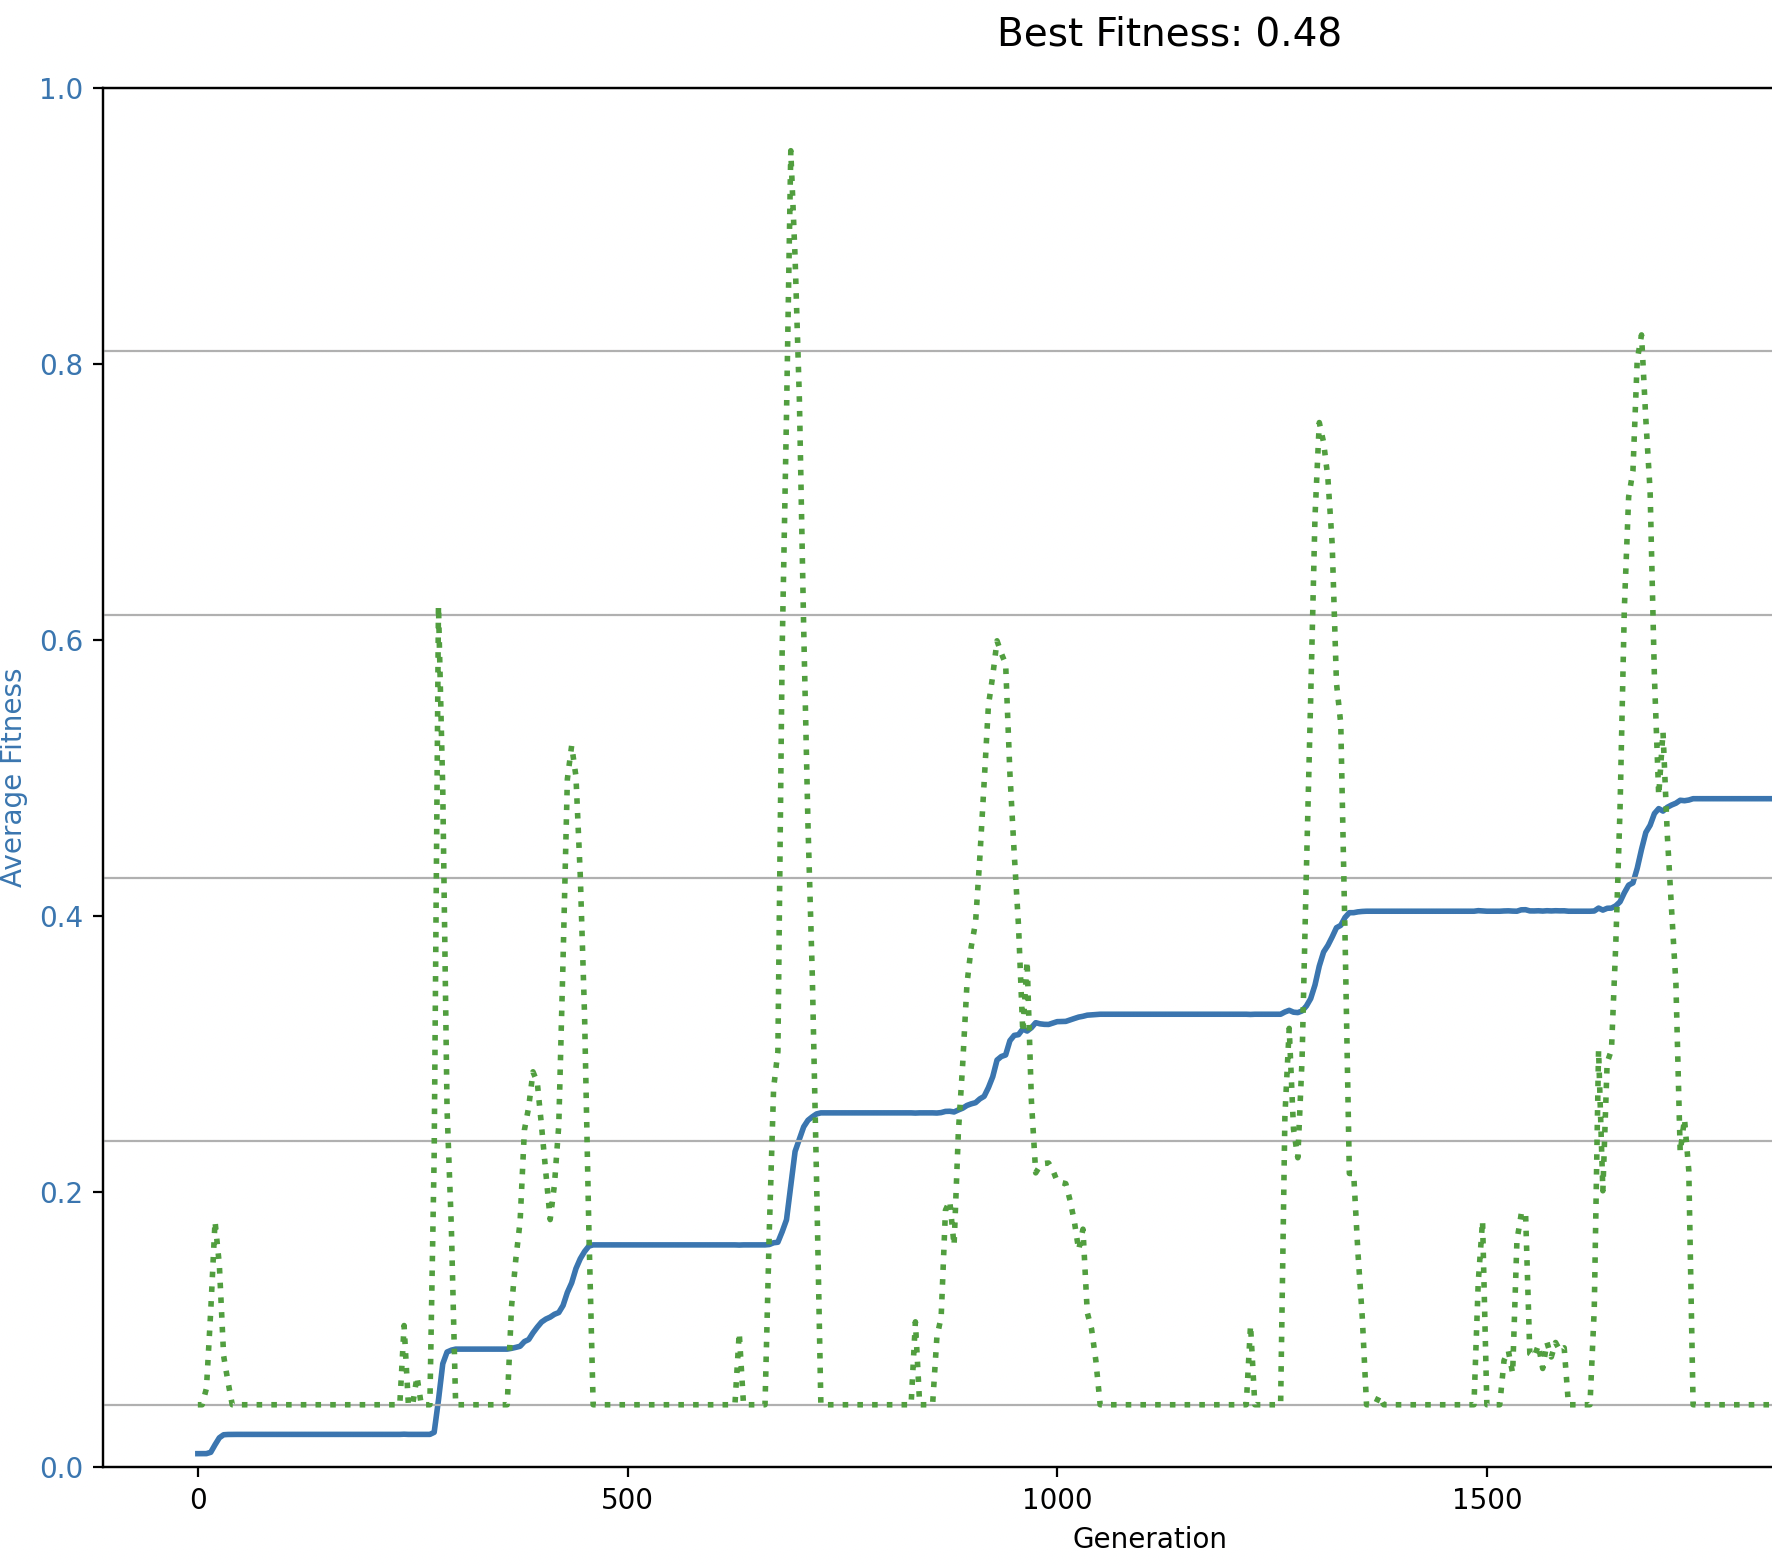
\includegraphics{images/evo_pract2_div.png}

\subsection{\texorpdfstring{Questions
Exercise~\ref{exr-evolving-dna}}{Questions Exercise~}}\label{questions-exr-evolving-dna}

\begin{enumerate}
\def\labelenumi{\alph{enumi}.}
\tightlist
\item
  The new blue dotted line represents how many mutations are beneficial
  (towards the target). As the population gets closer to the target, the
  number of beneficial mutations decreases. As such, this line is a
  mirror image of the fitness in the population. We will look a bit
  deeper into this line in the next model.
\item
  Generally speaking, a higher mutation rate helps to find the target
  faster. However, with high mutation rates (0.01 or higher), the
  fitness after the target is found starts to decrease, as individual
  produce many (unfit) mutants. In fact, if mutation rate is too high
  (approximately 0.04 or higher), the population fails to find the
  target at all, as reproduction is too inaccurate! This concept is
  known as the `error threshold' or the `error catastrophe' in
  evolutionary biology.
\item
  Qualitatively, there is no clear difference to what we saw before:
  diversity only peaks at moments when there is a new mutant coming in,
  but otherwise diversity is 0.
\item
  There is no distinction between genotype and phenotype. Fitness is
  directly calculated from the DNA sequence, so there is no
  `genotype-to-phenotype mapping'.
\end{enumerate}

\subsection{\texorpdfstring{Questions
Exercise~\ref{exr-evolving-proteins}}{Questions Exercise~}}\label{questions-exr-evolving-proteins}

\begin{enumerate}
\def\labelenumi{\alph{enumi}.}
\tightlist
\item
  The new black line is the maximum fitness in the population. Thanks to
  this line we can see that, sometimes, an individual is present that is
  fitter but it does not manage to take over the population. We are
  dealing with a stochastic process, so this is very natural.
\item
  The fitness line once again goes in distinct steps. The diversity line
  (green dotted) has a distinct behaviour compared to earlier models.
  Instead of only going up during the discovery of a new mutant, it
  constantly creeps up during periods where fitness does not change.
  This is because the codon-table is partially redundant: many different
  DNA sequences can code for the same amino acid sequence, so diveristy
  increases. However, when a new ``fitter'' individual comes in,
  diversity goes down as that individual clonally takes over the
  population. Then, diversity slowly increases again. A similar pattern
  is reflected in the line that represents the ``beneficial mutations''
  (blue dotted line). TLDR; even when fitness is not changing there is
  still a lot going on in this population!
\item
  This model represents a many-to-one mapping between genotype and
  phenotype. The DNA sequence (genotype) is translated into an amino
  acid sequence (phenotype), which is then used to calculate fitness.
  This means that many different genotypes can lead to the same
  phenotype, and thus the same fitness. Earlier in this course you have
  learned about development, and those processes often lead to effects
  where the same genotype can produce many different shapes
  (phenotypes).
\item
  \textbf{BONUS:} I have not personally done this, and I do not know the
  answer to this question yet. However, it is sometimes observed that
  with many-to-one mapping, populations can because better and better at
  switching between two alternating targets. This is because the
  alternating selection pressures make populations move towards
  genotypes that are ``close'' to both targets, and because there is
  some neutrality coding this can be acchieved without losing fitness in
  either environment. For cool paper on this principle, see Crombach and
  Hogeweg (2008). I suspect however that our current model will not be
  able to do the same.
\end{enumerate}

\section{Answers to Evolution Practical
3}\label{answers-to-evolution-practical-3}

This practical is quite open-ended, so instead of answers it is more
useful to have a scientific discussion. The image below was first run on
a spatially structured grid, but from the dashed line onwards the grid
was mixed every timestep. From this we can see that it matters ``who you
compete with''. On the spatial grid, individuals compete mostly with
other individuals of their own species. That means that, on average,
they cannot complement each other by providing public goods (they
produce the same set!). Because of this, the ``omni-producers'' (yellow
line) dominates, surrounded by a cloud of mutants that rely on other
types. The population size fluctuates strongly, as local populations can
collapse due to the loss of public goods, typically followed by the
``omni-producers'' once again invading the available niche space (empty
space on the grid).

When mixing the grid every time step, who you interact with is
randomised, and individuals can now rely on other genotypes in the
population. Although there is some luck involved in this, you can see
that the total population (the black line) increases from this point
onward. Thus, although the omni-producers are less dominant,
statistically individuals are much better off in this mixed world. That
said, there is a risk to this mixed population: if the cost of producing
public goods is too high, the population can collapse as there is a
strong incentive to lose production of public goods and start relying on
others. Depending on your implementation, you may find that mixed
systems therefor perform better \textbf{or} worse than spatially
structured systems. If they behave identically though, let me (Bram)
know, as that is something I almost never observe in models like this ;)

\begin{figure}[H]

{\centering 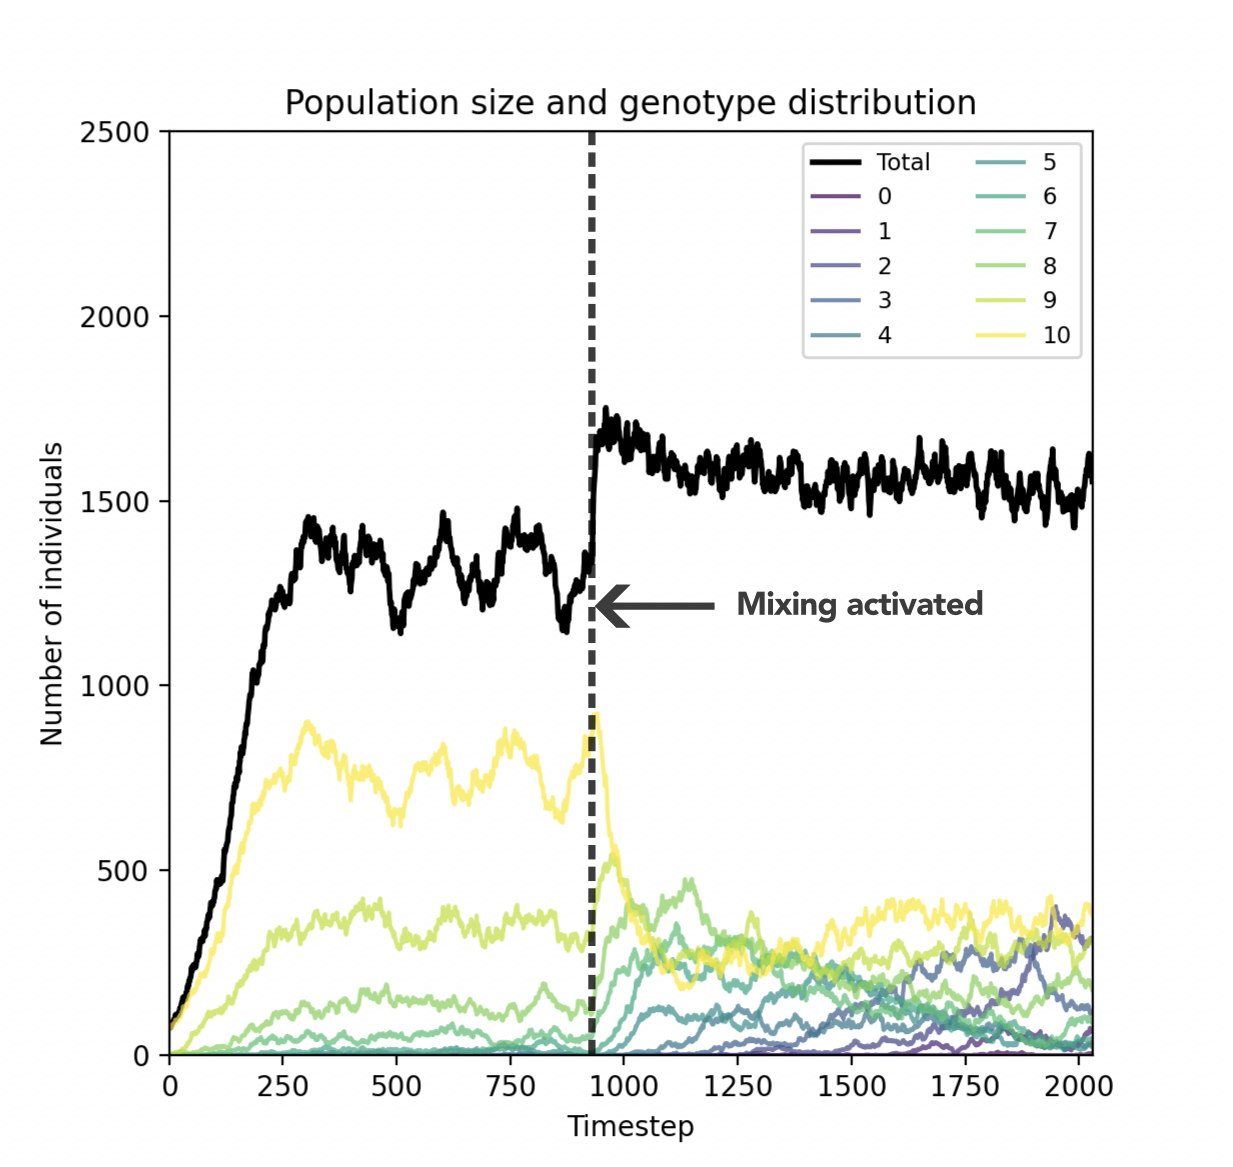
\includegraphics{images/evo_pract3_mix.png}

}

\caption{Dynamics of the producer-types in a system with 10 `public
goods'}

\end{figure}%

\part{Mini-projects}

\chapter{Differentiation
introduction}\label{differentiation-introduction-1}

\section{Equations}\label{equations-11}

Here's an equation:

\begin{equation}\phantomsection\label{eq-log}{ 
\frac{\mathrm{d}N}{\mathrm{d}t} = rN(1 - \frac{N}{K}) 
}\end{equation}

And Equation~\ref{eq-log} is a reference to the equation above.

\section{References}\label{references-11}

See Knuth (1984) for additional discussion of literate programming.

\section{Syntax highlighting}\label{syntax-highlighting-11}

Here's some python code:

\begin{Shaded}
\begin{Highlighting}[]
\ImportTok{import}\NormalTok{ numpy }\ImportTok{as}\NormalTok{ np}
\NormalTok{np.random.seed(}\DecValTok{42}\NormalTok{)}
\NormalTok{a }\OperatorTok{=} \DecValTok{1} \OperatorTok{+} \DecValTok{2}
\NormalTok{b }\OperatorTok{=}\NormalTok{ a }\OperatorTok{+} \DecValTok{3}
\BuiltInTok{print}\NormalTok{(}\StringTok{"Hello"}\NormalTok{)}
\end{Highlighting}
\end{Shaded}

\section{Visualising data (R)}\label{visualising-data-r-11}

Here's an interactive plot generated with R:

\includegraphics{project_1_files/figure-pdf/unnamed-chunk-1-1.pdf}

\section{A youtube clip:}\label{a-youtube-clip-11}

\url{https://www.youtube.com/embed/wo9vZccmqwc}

\section{An `iframe' to a different page (e.g.~my
simulations)}\label{an-iframe-to-a-different-page-e.g.-my-simulations-11}

\subsection{Mermaid}\label{mermaid-11}

Diagrams (Mermaid syntax):

\begin{figure}

\centering{

\includegraphics[width=7.47in,height=2.27in]{project_1_files/figure-latex/mermaid-figure-1.png}

}

\caption{\label{fig-variables}Types of models}

\end{figure}%

Which can be referred to Figure~\ref{fig-variables}.

\subsection{Callouts}\label{callouts-11}

Call-outs can organise information and highlight important points.

\begin{tcolorbox}[enhanced jigsaw, leftrule=.75mm, colbacktitle=quarto-callout-note-color!10!white, coltitle=black, colback=white, left=2mm, bottomtitle=1mm, arc=.35mm, titlerule=0mm, breakable, bottomrule=.15mm, opacitybacktitle=0.6, colframe=quarto-callout-note-color-frame, title=\textcolor{quarto-callout-note-color}{\faInfo}\hspace{0.5em}{Note}, opacityback=0, toprule=.15mm, toptitle=1mm, rightrule=.15mm]

Note that there are five types of callouts, including: \texttt{note},
\texttt{warning}, \texttt{important}, \texttt{tip}, and
\texttt{caution}.

\end{tcolorbox}

\begin{tcolorbox}[enhanced jigsaw, leftrule=.75mm, colbacktitle=quarto-callout-tip-color!10!white, coltitle=black, colback=white, left=2mm, bottomtitle=1mm, arc=.35mm, titlerule=0mm, breakable, bottomrule=.15mm, opacitybacktitle=0.6, colframe=quarto-callout-tip-color-frame, title=\textcolor{quarto-callout-tip-color}{\faLightbulb}\hspace{0.5em}{Tip with Title}, opacityback=0, toprule=.15mm, toptitle=1mm, rightrule=.15mm]

This is an example of a callout with a title.

\end{tcolorbox}

\begin{tcolorbox}[enhanced jigsaw, leftrule=.75mm, colbacktitle=quarto-callout-caution-color!10!white, coltitle=black, colback=white, left=2mm, bottomtitle=1mm, arc=.35mm, titlerule=0mm, breakable, bottomrule=.15mm, opacitybacktitle=0.6, colframe=quarto-callout-caution-color-frame, title=\textcolor{quarto-callout-caution-color}{\faFire}\hspace{0.5em}{Expand To Learn About Collapse}, opacityback=0, toprule=.15mm, toptitle=1mm, rightrule=.15mm]

This is an example of a `folded' caution callout that can be expanded by
the user. You can use \texttt{collapse="true"} to collapse it by default
or \texttt{collapse="false"} to make a collapsible callout that is
expanded by default.

\end{tcolorbox}

\begin{tcolorbox}[enhanced jigsaw, leftrule=.75mm, colbacktitle=quarto-callout-tip-color!10!white, coltitle=black, colback=white, left=2mm, bottomtitle=1mm, arc=.35mm, titlerule=0mm, breakable, bottomrule=.15mm, opacitybacktitle=0.6, colframe=quarto-callout-tip-color-frame, title=\textcolor{quarto-callout-tip-color}{\faLightbulb}\hspace{0.5em}{Tip \ref*{tip-example}: Cross-Referencing a Tip}, opacityback=0, toprule=.15mm, toptitle=1mm, rightrule=.15mm]

\quartocallouttip{tip-example} 

Add an ID starting with \texttt{\#tip-} to reference a tip.

\end{tcolorbox}

See Tip~\ref{tip-example}\ldots{}

\subsection{How to format questions/problem
sets}\label{how-to-format-questionsproblem-sets-11}

\begin{exercise}[Test
1]\protect\hypertarget{exr-test1}{}\label{exr-test1}

The equation of any straight line, called a linear equation, can be
written as:

\begin{equation}\phantomsection\label{eq-line}{ 
y = mx + b
}\end{equation}

Refer to the equation like this Equation~\ref{eq-line} or like
Customlabel~\ref{eq-line}.

\textbf{a.} Blabla?

\textbf{b.} Of blablabla?

\end{exercise}

\subsection{Sharing data tables:}\label{sharing-data-tables-11}

\includegraphics{project_1_files/figure-pdf/tab-anscombe-1.pdf}

\chapter{Miniproject: maintaining a healthy
microbiome}\label{miniproject-maintaining-a-healthy-microbiome}

\section{Mini description}\label{mini-description}

Microbes often form intricate relationships, not only amongst each
other, but also with larger organisms from all kingdoms: plants,
animals, and fungi. While they often provide useful services, microbes
typically evolve much faster than these hosts. What stops a microbe from
taking advantage of its host, taking more resources than it provides, or
even damaging the host tissue to gain access to even more resources? The
latter scenario, we would call a pathogen, and the likelyhood of this
transition from occuring could be called the \textbf{disease pressure}.

Understanding the fundamental principles behind disease pressure can
help mitigating disease outbreaks. For example, if we understand the
conditions under which a microbe is likely to become a pathogen, we can
take steps to prevent this from happening.

\begin{figure}

\centering{

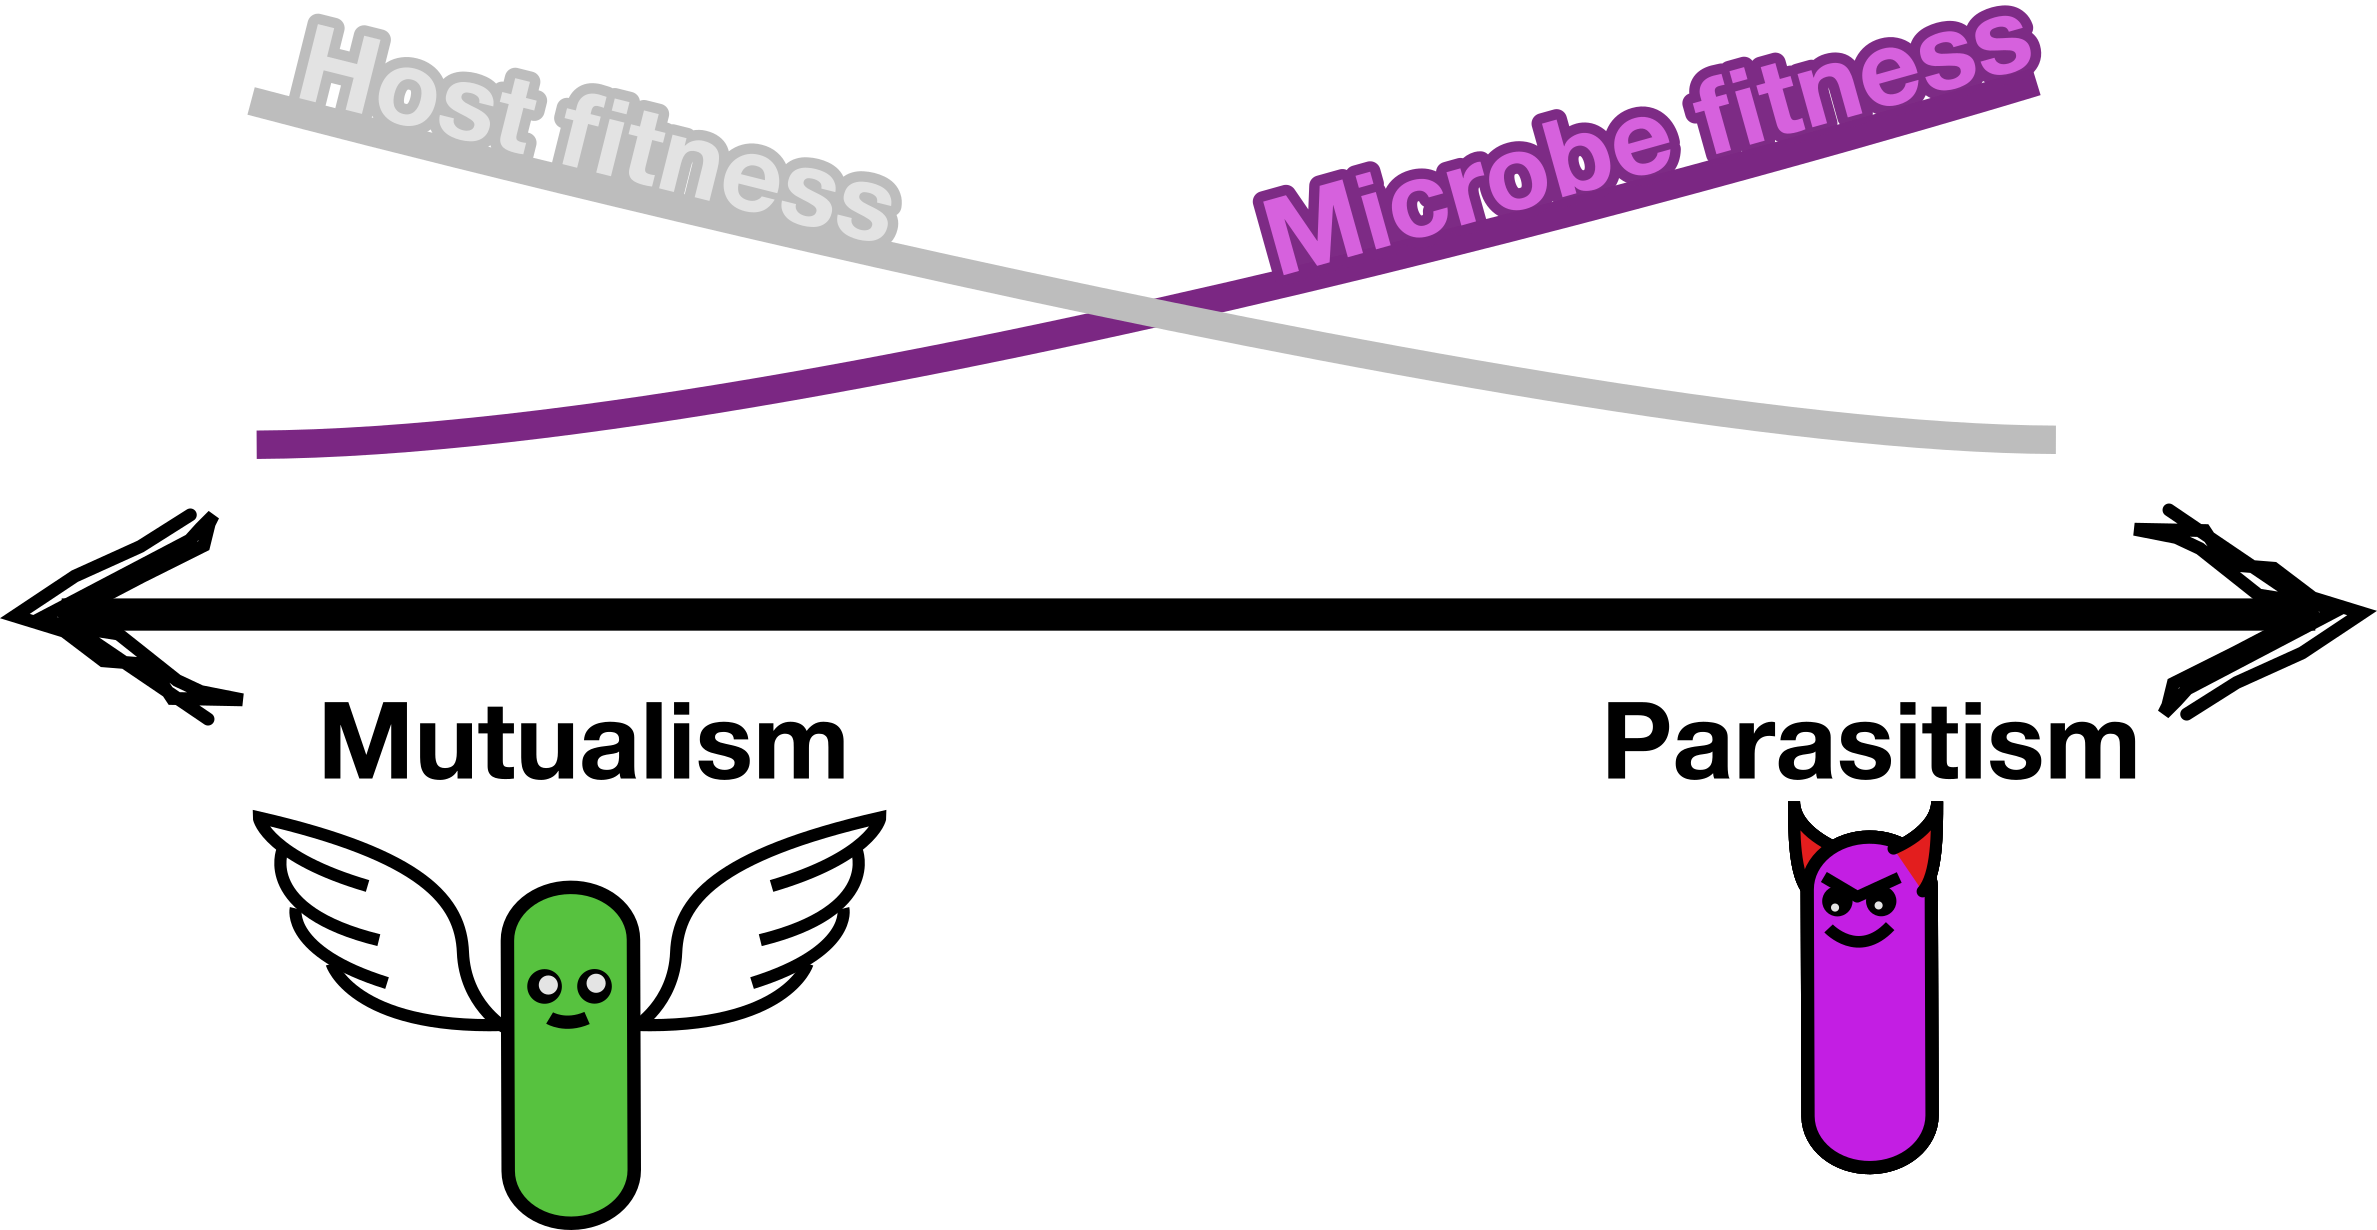
\includegraphics{images/mutpar_continuum.png}

}

\caption{\label{fig-parmut}Parasitism-mutualism continuum of
host-associated microbes. Note that this is a cartoon, and that nature
is in almost all cases more complicated than this.}

\end{figure}%

To phrase the above story a little differently: the microbes in our gut
or in the soil of our favourite crops, are constantly evolving on a
parasitism-mutualism continuum (see Figure~\ref{fig-parmut}). In this
mini project, you will investigate the dynamics of microbiomes evolving
on such a continuum. We will particularly focus on how the properties of
the \emph{host} (plant, animals, etc.) shape the likelihood of disease
outbreaks. To that end, here are a few key questions to get you started,
but you don't need to focus on each and every one of them at the same
time. Plus, more (better!) questions will likely emerge as you work on
the project. That's science.

\section{Key references}\label{key-references}

\begin{itemize}
\tightlist
\item
  Van Vliet and Doebeli (2019): a model of self-sacrificing microbes in
  hosts with different transmission modes.
\item
  Koskella and Bergelson (2020): an opinion piece on host-microbe
  (co)evolution and levels of selection
\end{itemize}

\section{Guiding questions:}\label{guiding-questions}

\begin{itemize}
\tightlist
\item
  Do motile hosts (e.g.~animals) experience different disease pressures
  than non-motile hosts (e.g.~plants)?
\item
  Are mutualistic microbes easier to maintain in short- or long-lived
  hosts?
\item
  Does non-local reproduction (e.g.~seed/spore dispersal) change these
  patterns?
\item
  How does an adaptive immune system (animals) affect the evolution of
  microbiomes, compared to plants, who don't have an adaptive immune
  system?
\end{itemize}

\section{Getting started}\label{getting-started}

Maintaining self-sacrificial microbiomes isn't easy, as shown by the
work of Van Vliet and Doebeli (2019). They show that the evolution of
self-sacrificing microbes (which they call ``helpers'') is highly
sensitive to the host's longevity and transmission of microbes in
between hosts (horizontal transmission). To understand why, start by
reading their paper. If you have read it, unfold the text below to see
my summary of their methods.

\begin{tcolorbox}[enhanced jigsaw, leftrule=.75mm, colbacktitle=quarto-callout-note-color!10!white, coltitle=black, colback=white, left=2mm, bottomtitle=1mm, arc=.35mm, titlerule=0mm, breakable, bottomrule=.15mm, opacitybacktitle=0.6, colframe=quarto-callout-note-color-frame, title=\textcolor{quarto-callout-note-color}{\faInfo}\hspace{0.5em}{My summary of the model by van Vliet et al.}, opacityback=0, toprule=.15mm, toptitle=1mm, rightrule=.15mm]

This model studies the maintanance of self-sacrificial ``helper''
microbes. Here, I will refer to helpers as ``allies'' (A), as to clearly
differentiate it from ``hosts'' (H). Microbes that are not allies are
referred to as neutral (N).

Allies provide a benefit to their host, while neutral microbes do not.
The microbes are modelled with simple ordinary differential equations
(ODEs):

\[
\begin{aligned}
\color{#555}{
\frac{dN}{dt} =
\underbrace{rN}_{\textrm{Growth N}} -
\underbrace{\delta N(A+N)}_{\textrm{Density-dependent death}}
}\\
\color{green}{
  \frac{dA}{dt} =
  \underbrace{rA(1-\gamma)}_{\textrm{Growth A}} -
  \underbrace{\delta A(A+N)}_{\textrm{Density-dependent death}}
}\\
\end{aligned}
\tag{1}
\] As you can see, allies grow slower than neutral microbes and are
therefore at a competitive disadvantage, and will eventually be
outcompeted. To counter-act the loss of allies, van Vliet's model
considers selection at the level of the host. To achieve this, the birth
rate of hosts (\(B_i\)) depends on the frequency of allies A in the
microbiome:

\[
B_i = \frac{r}{G_H}(1+s_b\cdot \frac{A}{A+N})
\]

Here, \(G_H\) is a parameter that scales the host generation time w.r.t.
the growth rate of microbes (\(r\)), with \(G_H \gg r\) ensuring hosts
are long-lived compared to microbes. The term \(s_b\) is the maximum
benefit that hosts get from carrying the ally strain.

The death rate of hosts (\(D_i\)) increases linearly with the density of
hosts at any given time (\(H(t)\)), and is given by:

\[
D_i = \frac{r}{G_H} \frac{H(t)}{K_H}
\]

Where \(H(t)\) gives the number of hosts at a given time, and \(K_H\)
denotes the basal carrying capacity in the absence of allies. Note that
the true carrying capacity can be higher, as helpers increase the birth
rate of hosts.

Whenever a host reproduces, the microbiome is transmitted vertically to
their offspring. The frequency of allies in the offspring is sampled
from a normal distribution with mean \(f_A\):

\[
f_{offspring}  = \mathcal{N} (f_{A},\sigma^2),
\\\text{with } f_A = \frac{A}{A+N}
\]

To avoid negative ally frequencies, this number is truncated such that
\(0<A_{offspring}<1\). The total density in the newborn is set by
another parameter \(n_0\). The model by van Vliet also considers
``horizontal'' transmission of microbiomes, where \(f_A\) is not the
ally frequency in the parent, but the frequency of allies in the
microbiome of a \textbf{random} individual.

So far so good with all the math. Now the simulation\ldots{}

\subsection{The simulation loop}\label{the-simulation-loop}

\begin{enumerate}
\def\labelenumi{\arabic{enumi}.}
\item
  The birth and death rates of all hosts is calculated
\item
  Calculate the probability of a host-level event (birth/death)
  occurring
\item
  If an event occurs, draw a random event proportional to its
  probability.
\item
  Execute the event sampled in step 3
\item
  Update all the microbiome ODEs.
\end{enumerate}

\end{tcolorbox}

To start the project, we will first replicate van Vliet's results in
Python. As a guideline, use my model summary above. I am ready to help
where needed, but at this point in the course your experience should go
a long way! If the simulation works, see if you can reproduce the
following two figures:

\begin{figure}

\begin{minipage}{0.50\linewidth}

\centering{

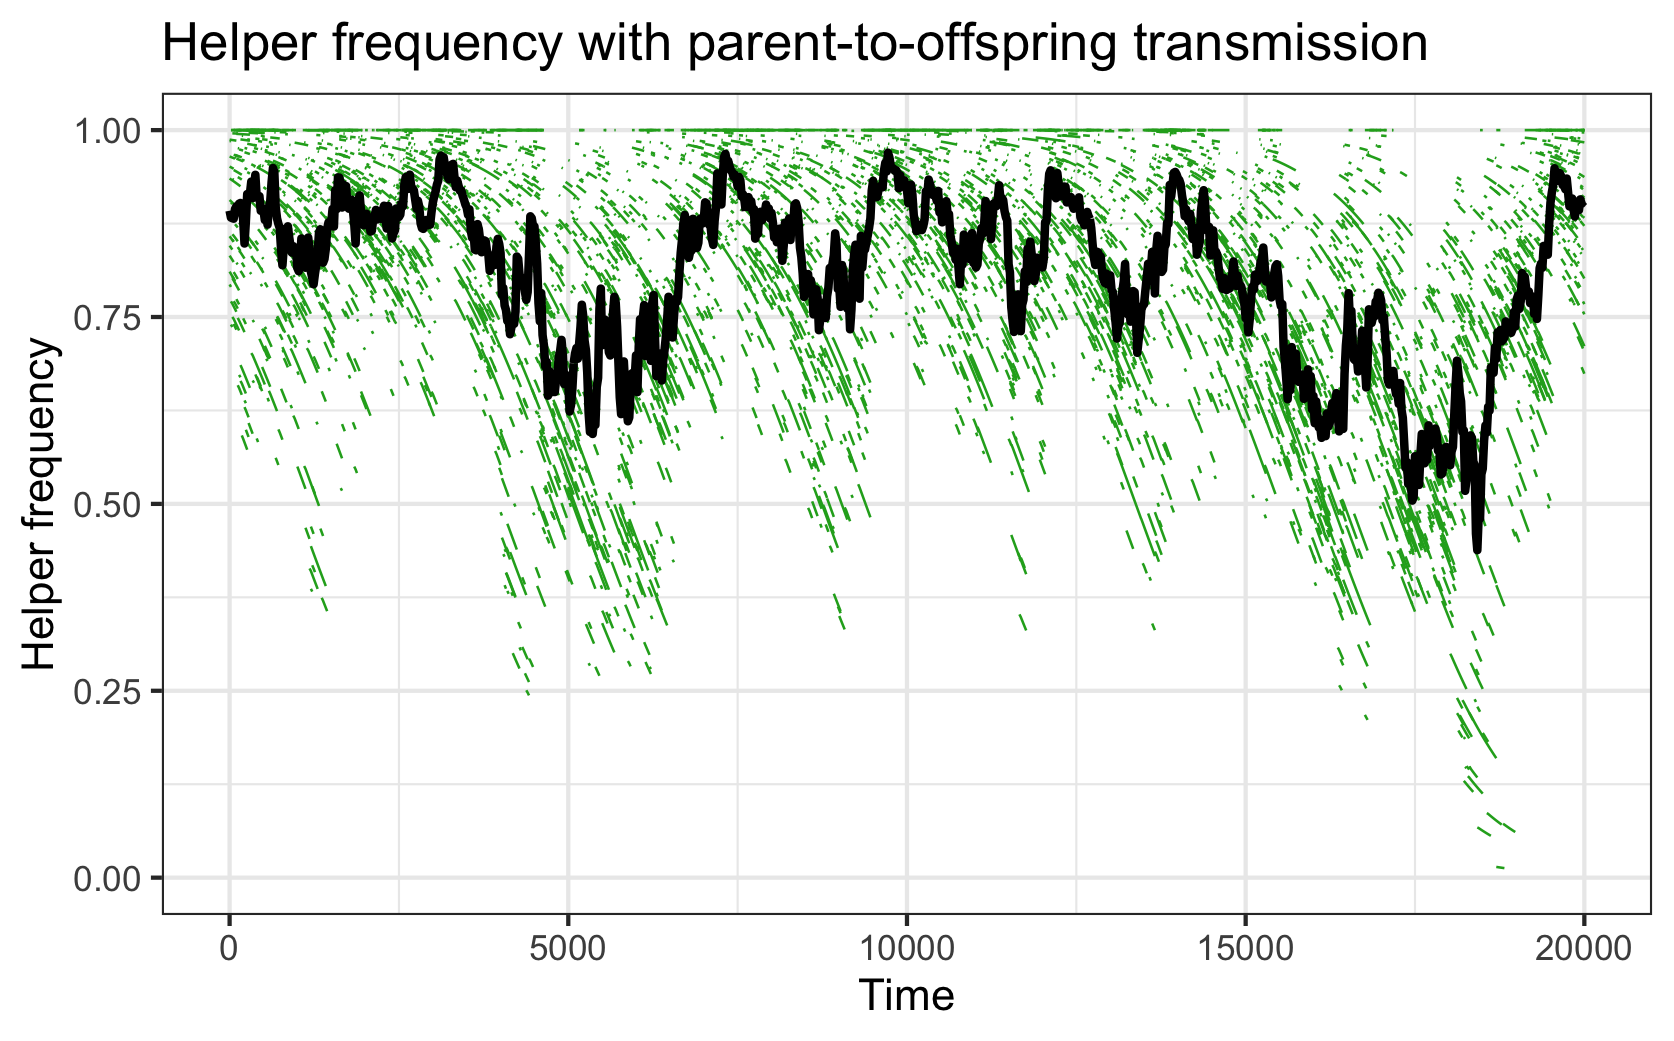
\includegraphics{images/vliet1.png}

}

\subcaption{\label{fig-vliet1}Allies are maintained within a population
of hosts (black line shows the average), despite each individual host
(green thinner lines) constantly decreasing in ally types. This can be
explained by selection at the level of the host.}

\end{minipage}%
%
\begin{minipage}{0.50\linewidth}

\centering{

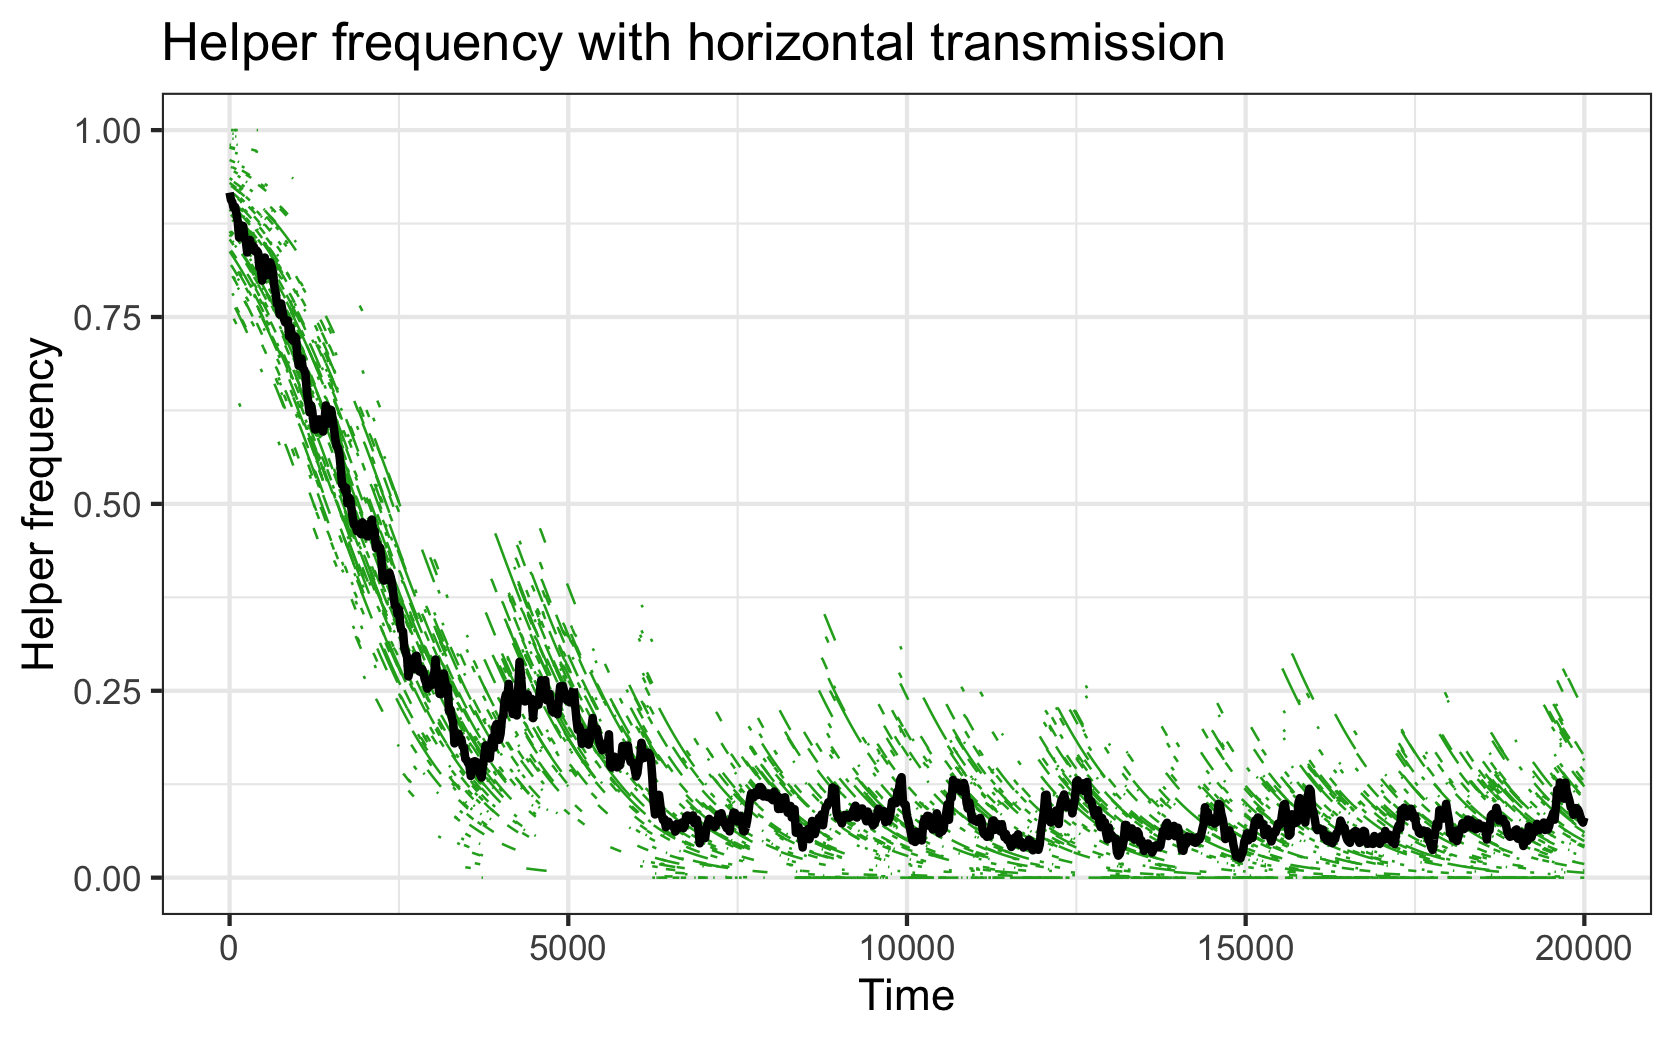
\includegraphics{images/vliet2.png}

}

\subcaption{\label{fig-vliet2}Allies are \emph{not} maintained within a
population of hosts (black line shows the average) when transmission of
microbiomes is horizontal (in between random individuals).}

\end{minipage}%

\caption{\label{fig-vliet}Helper maintenance in hosts with different
transmission modes}

\end{figure}%

\section{Extending the model}\label{extending-the-model}

Now that you have a working base-line model, let's extend it to address
the questions we phrased earlier: how does mobility of the host affect
the evolution of microbiomes, and what about non-locally reproducing
fungi? How do these host-level traits affect the likelyhood of
``disease'' outbreaks? Note that so far, we have only discussed
``helpers'' and ``neutral'' microbes, but the same principles apply to
pathogens but perhaps a little more extreme. For example, the microbes
may evolve such high levels of nastiness, that hosts do not only
replicate slower, but die. Think about ways to extend the model that
allows you to tune these distinctions.

\bookmarksetup{startatroot}

\chapter{Summary}\label{summary}

In summary, this book has no content whatsoever.

\begin{Shaded}
\begin{Highlighting}[]
\DecValTok{1} \OperatorTok{+} \DecValTok{1} \OperatorTok{=} \DecValTok{2}
\end{Highlighting}
\end{Shaded}

\bookmarksetup{startatroot}

\chapter*{References}\label{references-12}
\addcontentsline{toc}{chapter}{References}

\markboth{References}{References}

\phantomsection\label{refs}
\begin{CSLReferences}{1}{0}
\bibitem[\citeproctext]{ref-crombach2008evolution}
Crombach, Anton, and Paulien Hogeweg. 2008. {``Evolution of Evolvability
in Gene Regulatory Networks.''} \emph{PLoS Computational Biology} 4 (7):
e1000112.

\bibitem[\citeproctext]{ref-knuth84}
Knuth, Donald E. 1984. {``Literate Programming.''} \emph{Comput. J.} 27
(2): 97--111. \url{https://doi.org/10.1093/comjnl/27.2.97}.

\bibitem[\citeproctext]{ref-koskella2020study}
Koskella, Britt, and Joy Bergelson. 2020. {``The Study of
Host--Microbiome (Co) Evolution Across Levels of Selection.''}
\emph{Philosophical Transactions of the Royal Society B} 375 (1808):
20190604.

\bibitem[\citeproctext]{ref-van2019role}
Van Vliet, Simon, and Michael Doebeli. 2019. {``The Role of Multilevel
Selection in Host Microbiome Evolution.''} \emph{Proceedings of the
National Academy of Sciences} 116 (41): 20591--97.

\end{CSLReferences}

\cleardoublepage
\phantomsection
\addcontentsline{toc}{part}{Appendices}
\appendix

\chapter{Quarto examples}\label{quarto-examples-1}

\section{Equations}\label{equations-12}

Here's an equation:

\begin{equation}\phantomsection\label{eq-log}{ 
\frac{\mathrm{d}N}{\mathrm{d}t} = rN(1 - \frac{N}{K}) 
}\end{equation}

And Equation~\ref{eq-log} is a reference to the equation above.

\section{References}\label{references-13}

See Knuth (1984) for additional discussion of literate programming.

\section{Syntax highlighting}\label{syntax-highlighting-12}

Here's some python code:

\begin{Shaded}
\begin{Highlighting}[]
\ImportTok{import}\NormalTok{ numpy }\ImportTok{as}\NormalTok{ np}
\NormalTok{np.random.seed(}\DecValTok{42}\NormalTok{)}
\NormalTok{a }\OperatorTok{=} \DecValTok{1} \OperatorTok{+} \DecValTok{2}
\NormalTok{b }\OperatorTok{=}\NormalTok{ a }\OperatorTok{+} \DecValTok{3}
\BuiltInTok{print}\NormalTok{(}\StringTok{"Hello"}\NormalTok{)}
\end{Highlighting}
\end{Shaded}

\section{Visualising data (R)}\label{visualising-data-r-12}

Here's an interactive plot generated with R:

\includegraphics{answers_files/figure-pdf/unnamed-chunk-1-1.pdf}

\section{A youtube clip:}\label{a-youtube-clip-12}

\url{https://www.youtube.com/embed/wo9vZccmqwc}

\section{An `iframe' to a different page (e.g.~my
simulations)}\label{an-iframe-to-a-different-page-e.g.-my-simulations-12}

\subsection{Mermaid}\label{mermaid-12}

Diagrams (Mermaid syntax):

\begin{figure}

\centering{

\includegraphics[width=7.47in,height=2.27in]{answers_files/figure-latex/mermaid-figure-1.png}

}

\caption{\label{fig-variables}Types of models}

\end{figure}%

Which can be referred to Figure~\ref{fig-variables}.

\subsection{Callouts}\label{callouts-12}

Call-outs can organise information and highlight important points.

\begin{tcolorbox}[enhanced jigsaw, leftrule=.75mm, colbacktitle=quarto-callout-note-color!10!white, coltitle=black, colback=white, left=2mm, bottomtitle=1mm, arc=.35mm, titlerule=0mm, breakable, bottomrule=.15mm, opacitybacktitle=0.6, colframe=quarto-callout-note-color-frame, title=\textcolor{quarto-callout-note-color}{\faInfo}\hspace{0.5em}{Note}, opacityback=0, toprule=.15mm, toptitle=1mm, rightrule=.15mm]

Note that there are five types of callouts, including: \texttt{note},
\texttt{warning}, \texttt{important}, \texttt{tip}, and
\texttt{caution}.

\end{tcolorbox}

\begin{tcolorbox}[enhanced jigsaw, leftrule=.75mm, colbacktitle=quarto-callout-tip-color!10!white, coltitle=black, colback=white, left=2mm, bottomtitle=1mm, arc=.35mm, titlerule=0mm, breakable, bottomrule=.15mm, opacitybacktitle=0.6, colframe=quarto-callout-tip-color-frame, title=\textcolor{quarto-callout-tip-color}{\faLightbulb}\hspace{0.5em}{Tip with Title}, opacityback=0, toprule=.15mm, toptitle=1mm, rightrule=.15mm]

This is an example of a callout with a title.

\end{tcolorbox}

\begin{tcolorbox}[enhanced jigsaw, leftrule=.75mm, colbacktitle=quarto-callout-caution-color!10!white, coltitle=black, colback=white, left=2mm, bottomtitle=1mm, arc=.35mm, titlerule=0mm, breakable, bottomrule=.15mm, opacitybacktitle=0.6, colframe=quarto-callout-caution-color-frame, title=\textcolor{quarto-callout-caution-color}{\faFire}\hspace{0.5em}{Expand To Learn About Collapse}, opacityback=0, toprule=.15mm, toptitle=1mm, rightrule=.15mm]

This is an example of a `folded' caution callout that can be expanded by
the user. You can use \texttt{collapse="true"} to collapse it by default
or \texttt{collapse="false"} to make a collapsible callout that is
expanded by default.

\end{tcolorbox}

\begin{tcolorbox}[enhanced jigsaw, leftrule=.75mm, colbacktitle=quarto-callout-tip-color!10!white, coltitle=black, colback=white, left=2mm, bottomtitle=1mm, arc=.35mm, titlerule=0mm, breakable, bottomrule=.15mm, opacitybacktitle=0.6, colframe=quarto-callout-tip-color-frame, title=\textcolor{quarto-callout-tip-color}{\faLightbulb}\hspace{0.5em}{Tip \ref*{tip-example}: Cross-Referencing a Tip}, opacityback=0, toprule=.15mm, toptitle=1mm, rightrule=.15mm]

\quartocallouttip{tip-example} 

Add an ID starting with \texttt{\#tip-} to reference a tip.

\end{tcolorbox}

See Tip~\ref{tip-example}\ldots{}

\subsection{How to format questions/problem
sets}\label{how-to-format-questionsproblem-sets-12}

\begin{exercise}[Test
1]\protect\hypertarget{exr-test1}{}\label{exr-test1}

The equation of any straight line, called a linear equation, can be
written as:

\begin{equation}\phantomsection\label{eq-line}{ 
y = mx + b
}\end{equation}

Refer to the equation like this Equation~\ref{eq-line} or like
Customlabel~\ref{eq-line}.

\textbf{a.} Blabla?

\textbf{b.} Of blablabla?

\end{exercise}

\subsection{Sharing data tables:}\label{sharing-data-tables-12}

\includegraphics{answers_files/figure-pdf/tab-anscombe-1.pdf}




\end{document}
